\documentclass[11pt,a4paper]{article}
\usepackage[a4paper, left=2.5cm, right=2.5cm, top=2.5cm, bottom=2.5cm]{geometry}
\usepackage{setspace}
\setstretch{1.15}  % Interligne 1.15

\usepackage{tocbibind} % Pour inclure la table des matières automatiquement
\usepackage{fancyhdr}
\usepackage{graphicx}
\usepackage{xcolor}
\usepackage{enumitem} % Permet de personnaliser les listes
\usepackage[T1]{fontenc} % Assure une bonne gestion des caractères
\usepackage[utf8]{inputenc} % Encodage UTF-8
\setcounter{secnumdepth}{5} % Numérotation jusqu'au niveau 4
\setcounter{tocdepth}{5}    % Ajout à la table des matières
\usepackage[hidelinks]{hyperref} % Active les liens sans encadré coloré
\usepackage{float} % À mettre dans le préambule
\usepackage{titling} % Nécessaire pour \subtitle
%\usepackage{amssymb}
\usepackage{enumitem} % à placer dans le préambule

\usepackage[utf8]{inputenc}
\usepackage[T1]{fontenc}
\usepackage[french]{babel}
\frenchbsetup{StandardLists=true} % à inclure si on utilise \usepackage[french]{babel}

\begin{document}
\pagenumbering{gobble} % Supprime les numéros de page
\onehalfspacing

\begin{minipage}[t]{0.4\textwidth}
    \vspace{0pt} % force l’alignement en haut
    
\includegraphics[width=5cm]{../Images/logo-sup.jpg}
\end{minipage}
\hfill
\begin{minipage}[t]{0.6\textwidth}
    \vspace{0pt}
    \raggedleft
    
\includegraphics[width=5cm]{../Images/logo.png}
\end{minipage}

\vspace{2cm}

\begin{center}
    \LARGE \textbf{Mémoire de fin d'études}\\[1em]
    \Large Mastère 2\textsuperscript{ème} année\\[1em]
    \Large Spécialisation : Développement Full-Stack \\[3em]

   % \huge \textbf{Conception et développement d’applications web sur mesure pour la digitalisation des processus industriels chez Jeumont Electric}\\[2em]
   
   \huge \textbf{Digitalisation de processus industriels par des applications web sur mesure : retour d’expérience chez Jeumont Electric}\\[2em]
    \Large Aboubacar Sidiki CONDE
\end{center}

\vfill

\begin{flushleft}
    \textbf{Maître(s) d’apprentissage entreprise :} Mme Katia BION et M. Stéphane DESHAIES\\[1em]
    \textbf{Coach(s) :} Mme Hélène LIONNET \\[1em]
    \textbf{Responsable pédagogique :} Mme Hélène LIONNET
\end{flushleft}

\newpage
\pagenumbering{arabic} % Reprend la numérotation des pages
\setcounter{page}{2}

\newpage
\begin{center}
\section*{Dédicaces}
\Large
\textit{%
Avec l’expression de ma reconnaissance, je dédie ce modeste travail et\\
ma profonde gratitude à ma très chère mère \textbf{Saran Camara} et à mon\\
père \textbf{Souleymane Condé} pour l’éducation qu’ils m’ont prodiguée,\\
avec tous les moyens et au prix de tous les sacrifices qu’ils ont consentis à mon égard depuis mon enfance.}

\textit{Vous qui m’avez toujours soutenu tant moralement que financièrement dans des moments difficiles, je ne saurais vous dire que merci pour l’accomplissement de votre devoir.\\[1em]}

\textit{À la mémoire de maman \textbf{Mariame Gbati Cissé}, puisse Dieu le tout\\
puissant lui accorde sa clémence et sa miséricorde.\\[1em]}

\textit{À mes frères et sœurs \textbf{Mamadi Saran Condé}, \textbf{Alassane Keïta} et\\
\textbf{Mariame Condé} pour leur soutien moral et financier en témoignage\\
de l’attachement, de l’amour et de l’affection que je leur porte.\\[1em]}

\textit{À tous mes amis pour tous les instants inoubliables que j’ai passés\\
avec vous, je vous remercie. À tous mes professeurs en témoignage de\\
ma gratitude et profond respect.}

\vspace{2cm}

\begin{flushright}
\Large
\textit{Aboubacar Sidiki Condé}
\end{flushright}
\end{center}

\newpage
\begin{center}
\Large
\section*{Remerciements}
\textit{
Dans le cadre de ce travail, je tiens à adresser mes chaleureux\\
remerciements à mon encadrant pédagogique de \textbf{Sup de Vinci de Nantes}, Monsieur} \textit{ \textbf{Pascal BERNARD} pour tous les conseils qu’il m’a prodigués durant l’élaboration de ce travail.\\[1em]}

\textit{Mes remerciements vont à Monsieur \textbf{David RABAU}, directeur du site de \textit{Jeumont Electric Carquefou}, pour m’avoir accueilli afin d'effectuer mon alternance, \textbf{Madame Katia BION} et \textbf{Monsieur Stéphane DESHAIES},mes maitre d'apprentissage, pour leurs conseils avisés et le soutient qu’ils m’ont apporté.\\[1em]}

\textit{Merci également à tout le corps professoral, administratif et\\
technique de \textbf{Sup de Vinci de Nantes}, pour la qualité de l’enseignement\\
qui nous a été dispensé et le séjour agréable tout au long de ces années.\\[1em]}

\textit{Je tiens à exprimer ma reconnaissance envers mes camarades de formation et mes collègues de Jeumont Electric,\\
avec qui j’ai partagé des moments mémorables et des échanges fructueux.\\
Vos perspectives diverses et vos compétences uniques ont enrichi mon expérience
et ont fait de cette période d’alternance un chapitre inoubliable de ma formation.\\[1em]}

\textit{Enfin, je n’oublierai pas de remercier ma famille, mes amis et mes proches\\
pour leur soutien constant, leurs encouragements et leurs précieux conseils.
Votre présence à mes côtés m’a donné la force nécessaire pour relever les défis
et saisir les opportunités qui se sont présentées.}
\end{center}

\newpage
\section*{Avant-propos}
\addcontentsline{toc}{section}{Avant-propos}
\thispagestyle{empty}
\setstretch{1.3}
\begin{flushleft}
Ce mémoire s’inscrit dans le cadre de ma formation en \textbf{Mastère 2 Développement Full-Stack} à \textbf{Sup de Vinci Nantes}, et retrace l’expérience vécue au sein de l’entreprise \textbf{Jeumont Electric} situé en Loire Atlantique, sur le site de Carquefou, dans le cadre de mon alternance.

\vspace{0.5em}
Il ne s’agit pas uniquement d’un travail technique centré sur la conception d’applications web, mais bien d’un projet à forte portée humaine, organisationnelle et stratégique. L’objectif a été de répondre à des besoins concrets du terrain, en apportant des solutions numériques utiles, évolutives et adaptées aux réalités industrielles.

\vspace{0.5em}
Ce travail m’a permis d'approfondir mes compétences techniques en développement web (\textit{back-end}, \textit{front-end}, bases de données, architecture logicielle), tout en m’ouvrant aux enjeux de transformation numérique dans un environnement industriel exigeant. Il m’a aussi permis d’apprendre à écouter, à collaborer avec des équipes pluridisciplinaires, à documenter mes actions, à m’adapter aux contraintes, et à piloter des projets dans un cadre professionnel réel.

\vspace{0.5em}
Je tiens à préciser que ce mémoire n’a pas pour ambition d’être une vérité absolue, mais une contribution personnelle, enrichie par l’observation, la pratique et les échanges menés tout au long de cette alternance. Il reflète à la fois mes apprentissages, mes questionnements et ma volonté de participer activement à la modernisation des processus industriels à travers le levier du numérique.

\vspace{0.5em}
Ce document est aussi l’aboutissement d’un accompagnement bienveillant, de l’encadrement pédagogique de \textbf{Sup de Vinci} et du soutien quotidien de mes référents chez \textbf{Jeumont Electric}. Il témoigne de ce que peut être une alternance réussie : un pont entre la théorie et la pratique, entre les exigences académiques et les besoins de l’entreprise, entre les lignes de code et les impacts concrets sur le terrain.
\end{flushleft}

\newpage
\begin{spacing}{1} % facultatif pour compresser aussi l'interligne
	\renewcommand{\contentsname}{Table des matières}
	{\normalsize
	\tableofcontents}
\end{spacing}

\newpage

\renewcommand{\listfigurename}{Tables des images}
\listoffigures

\newpage
\listoftables

\newpage
\section*{Introduction générale}
\addcontentsline{toc}{section}{Introduction générale}

La transformation entrée numérique transforme en véritable profondeur le fonctionnement des entreprises industrielles. Ce mouvement, généralement appelé industrie 4.0, repose sur un usage croissant des technologies de l’information utilisé dans les processus de production, de maintenance, de pilotage etc. Dans un environnement de plus en plus concurrentiel, les entreprises doivent composer avec des exigences de qualité, de traçabilité, de réactivité et d’optimisation des ressources de plus en plus élevées. 

Ce changement implique non seulement des outils, mais autant remettre à plat des pratiques, augmenter les capacités à exploiter les données et surtout adapter les solutions aux réalités locales du commerce. Les applications Web personnalisées participent valorise cette démarche, puisqu’elles sont développées au plus près des besoins des utilisateurs par qui des processus encore basiquement traitées traditionnelles, avec des outils de type bureautique ancien, des bases de données locales jusqu’à et morcelées, ou des programmes papiers difficilement utilisables, sont remodelés.

Jeumont Electric, acteur reconnu dans le domaine des machines électriques tournantes de forte puissance, n’échappe pas à ces enjeux.  Son site de Carquefou, où sont menées les opérations de maintenance, les expertises techniques et la rénovation d’équipements critiques, était encore en grande partie caractérisé par des processus utilisant des outils inadaptés aux exigences d'aujourd’hui. Les services concernés, maintenance, production, technique faisaient face à des limites concrètes : absence de centralisation et du maîtrise du flux de production, manque de traçabilité, surcharge administrative, difficulté à piloter les coûts en temps réel.


C’est dans ce contexte qu’a été définie la mission de ce mémoire. En tant qu’alternant en Mastère Développement Full-Stack,  j’étais en charge, de la conception du développement et de la mise en œuvre de plusieurs applications web sur mesure pour moderniser les processus internes du site de Carquefou. Cette mission est réalisée dans un projet Agile, orienté sur les utilisateurs finaux, avec une démarche de co-construction itérative.

La problématique à laquelle ce mémoire tente d’apporter une réponse est la suivante :

\begin{quote}
\emph{Comment concevoir et intégrer efficacement des applications web sur mesure pour moderniser des processus industriels critiques, tout en assurant leur adoption durable par les utilisateurs et en accompagnant la transformation numérique de l’entreprise sur les plans technique, humain et organisationnel ?
}
\end{quote}

Trois outils principaux ont été réalisés dans le cadre de cette mission :
\begin{itemize}
    \item Une application de \textbf{base d’expertise} pour centraliser et fiabiliser les rapports techniques,
    \item Une application de \textbf{traçabilité des barres} pour suivre les composants critiques de production,
    \item Une application de \textbf{suivi budgétaire maintenance} pour piloter en temps réel les coûts et interventions.
\end{itemize}

Chacun de ces outils a été pensé pour répondre à des besoins concrets exprimés par les utilisateurs, améliorer la fiabilité des données, alléger les tâches administratives, et faciliter la prise de décision. Leur déploiement progressif sur le site a permis d’ancrer la digitalisation dans le quotidien des équipes.

Ce mémoire est structuré en cinq chapitres. Après avoir présenté le contexte de l’entreprise et les enjeux de la mission (chapitre 1), nous verrons dans un deuxième chapitre quel ancrage industriel affecter à la digitalisation. Le chapitre 3 détaillera le cadrage de la mission ainsi que la méthode retenue. Le chapitre 4 traitera du développement technique des applications, avant que le chapitre 5 ne propose un bilan critique et des perspectives sous des éclairages qualitatifs et quantitatifs.


\newpage
\section{Présentation de Jeumont Electric}

Jeumont Electric est un acteur clé de l’électromécanique industrielle, notamment sur les segments stratégiques du nucléaire, de la marine et de la production d’énergie. Le site de Carquefou, où s’est déroulée ma mission, est spécialisé dans les expertises techniques et la maintenance lourde, un contexte favorable à la modernisation numérique ciblée. Filiale des groupes \textbf{Framatome} et \textbf{Naval Group}, Jeumont Electric s'appuie sur des savoir-faire historiques et des technologies propriétaires reconnues dans les secteurs de l'énergie,de la marine et de l'industrie lourde.

Créée il y a plus de \textbf{125 ans}, l'entreprise regroupe aujourd'hui environ \textbf{620 salariés} répartis sur quatre sites de production en France, et intervient dans plus de\textbf{ 70 pays à travers le monde}. Forte de son expertise et de sa capacité d'innovation, Jeumont Electric accompagne une clientèle internationale composée de grands groupes industriels, de chantiers navals, et d'opérateurs du secteur nucléaire.

Le siège historique de Jeumont Electric est situé à Jeumont, dans les Hauts-de-France. Tou-
tefois, l'entreprise dispose également d'un site stratégique à Carquefou, près de Nantes, dédié principalement aux activités d'expertise technique, de maintenance lourde et de rénovation
d'équipements électriques.

Le site de Carquefou occupe une place centrale dans la stratégie de l'entreprise. Il est reconnu
pour son savoir-faire en matière d'expertises électriques, de réconstruction de stators et de rotors, et
pour sa capacité à mener des projets de maintenance préventive et corrective de grande envergure, voir le site officiel\footnote{Jeumont Electric. \textit{Présentation de l’activité}. Disponible sur : \url{https://www.jeumontelectric.com} (consulté en avril 2025).}.

\begin{figure}[H]
    \centering
    
\includegraphics[width=0.8\textwidth]{../Images/logo.png}
    \caption{Logo de l'entreprise}
\end{figure}


\subsection{Missions et offre de services}

La mission de Jeumont Electric est de concevoir, fabriquer, maintenir et innover pour garantir le socle nucléaire, des machines électriques tournantes de forte puissance destinées aux secteurs stratégiques de l'énergie, du nucléaire, de la marine et de l'industrie lourde.
L'entreprise intervient tout au long du cycle de vie des équipements électriques, en proposant une gamme complète de produits et de services, parmi lesquels :

\begin{itemize}
    \item \textbf{Conception et fabrication} de machines neuves : alternateurs, moteurs électriques, générateurs de forte puissance.
    \item \textbf{Maintenance préventive et corrective} : interventions sur site ou en atelier pour assurer la fiabilité et la disponibilité des équipements.
    \item \textbf{Expertise et diagnostic} : inspections mécaniques et électriques pour anticiper les pannes, optimiser les performances et prolonger la durée de vie des machines.
    \item \textbf{Rénovation et modernisation} : remise à niveau technologique, remplacement de composants critiques, amélioration de la performance énergétique.
    \item \textbf{Fourniture de pièces de rechange} : standard ou spécifiques, y compris pour des équipements d’autres marques et maintenance lourde.
    \item \textbf{Conseil technique et accompagnement} : audits, études de faisabilité, recommandations pour l’optimisation industrielle.
\end{itemize}

Jeumont Electric fonde son approche sur un haut niveau d'expertise technique, une capacité à s'adapter aux spécificités de chaque projet, et un engagement fort en matière de qualité, de sécurité et de respect des délais. Son offre de service repose également sur une proximité forte avec ses clients, rendue possible par la présence de plusieurs sites de production et de centres de service, notamment à Jeumont et Carquefou, mais aussi par des interventions régulières à l'international.

Grâce à ses compétences reconnues et à ses technologies propriétaires, Jeumont Electric
accompagne ses partenaires industriels dans leurs projets de construction neuve, d'extension de
parc, de maintien en conditions opérationnelles ou d'amélioration de la performance énergétique.

\subsection{Le site de Carquefou : un centre stratégique}

Situé près de Nantes, le site de Carquefou est un des pôles clés de l’entreprise. Il concentre les activités liées à la maintenance lourde, aux expertises techniques (électriques et mécaniques), et à la rénovation des équipements tournants.

Ce site est particulièrement reconnu pour :
\begin{itemize}
    \item son savoir-faire dans la réparation de stators et rotors ;
    \item sa capacité à gérer des projets de maintenance de grande envergure ;
    \item ses interventions sur des équipements critiques pour des clients comme ArcelorMittal ou Framatome.
    \item la production des barres Roebel.
\end{itemize}

C’est également à Carquefou qu’a été menée la mission de digitalisation qui constitue le cœur de ce mémoire. Ce site incarne les problématiques rencontrées par de nombreuses industries : coexistence de savoir-faire pointus avec des outils de gestion parfois datés, et besoin croissant de structurer l’information technique pour renforcer le pilotage et la performance.

\subsection{Chiffres clés}
Quelques chiffres illustratifs de l'importance de Jeumont Electric dans son secteur :
Jeumont Electric dispose de plus de \textbf{120 ans d'expérience} industrielle et regroupe en viron \textbf{620 collaborateurs} répartis sur plusieurs sites en France, dont Jeumont et Carquefou.
L'entreprise est présente dans plus de \textbf{70 pays à travers le monde} et assure le suivi de plus de \textbf{3 500 machines électriques} installées. Son chiffre d'affaire annuel avoisine les \textbf{150 millions d'euros}, dont plus de \textbf{30 \% }est réalisé à l'international.

Ces éléments témoignent de la solidité financière, du savoir faire technique et de la capacité d'innovation de Jeumont Electric, qui demeure un acteur incontournable dans les domaines de l'énergie, de la marine, du ferroviaire et de l'industrie lourde.

\begin{table}[H]
\centering
\begin{tabular}{|p{8cm}|p{5cm}|}
	\hline
	\textbf{Indicateur} & \textbf{Valeur} \\ \hline
	Année de création & 1898 \\ \hline
	Collaborateurs & Environ 620 \\ \hline
	Présence géographique & Plus de 70 pays \\ \hline
	Machines installées & Plus de 3 500 \\ \hline
	Chiffre d'affaires annuel & Environ 150 M€ \\ \hline
	Part du CA à l'international & Plus de 30\,\% \\ \hline
\end{tabular}
\caption{Chiffres clés de Jeumont Electric}
\end{table}


\subsection{Organigramme de Carquefou}
L’établissement secondaire de Jeumont Electric à Carquefou est structuré autour d’une organisation fonctionnelle clairement définie. Chaque service a un rôle spécifique dans le bon déroulement des opérations industrielles, administratives et techniques du site. Cette organisation favorise la transversalité, la communication entre pôles, et l'efficacité des processus internes.

L’organigramme ci-dessous illustre la répartition des services et la position de l’alternant dans la hiérarchie fonctionnelle :

\begin{figure}[H]
    \centering
    \includegraphics[width=\textwidth]{../Images/organigramme.png}
    \caption{Organigramme de Jeumont Electric - Carquefou}
\end{figure}

Voici les principaux services présents sur le site :

\begin{itemize}
    \item \textbf{Chef d’Établissement} : assure la direction globale du site, l’arbitrage stratégique et la coordination entre services.

    \item \textbf{Service RH} : gère le recrutement, la gestion administrative du personnel et le développement des compétences.
    \item \textbf{Service QSE (Qualité, Sécurité, Environnement)} : responsable de la conformité aux normes, de la prévention des risques et de l'amélioration continue.
    \item \textbf{Service Maintenance} : en charge des opérations de maintenance préventive et corrective sur les équipements.
    \item \textbf{Service Achats et Stratégie} : gère les relations fournisseurs, les approvisionnements et la stratégie d'achat.
    \item \textbf{Service Administratif et Financier} : assure la gestion comptable, le contrôle de gestion, et le suivi budgétaire.
    \item \textbf{Service Production} : supervise les ateliers de fabrication, de bobinage, d’essais, et de connexions mécaniques.
    \item \textbf{Service Projets et Chantiers} : coordonne les projets industriels, les interventions sur site, et le suivi technique.
    \item \textbf{Service Technique} : apporte un support technique aux opérations, propose des solutions aux problématiques complexes.
    \item \textbf{Service Support Opérations} : soutien logistique et opérationnel aux équipes de production et de maintenance.
    \item \textbf{Service Marketing et Commercial} : en charge de la relation client, des appels d’offres et du développement commercial.
    \item \textbf{Pôle Marine Militaire} : pilote les projets spécifiques pour les clients militaires, notamment dans le secteur naval.
\end{itemize}

Mon rôle d’alternant développeur s’inscrit au sein du \textbf{service maintenance et production }, sous la responsabilité de Mme Katia BION. Cette position m’a permis de travailler de manière transversale avec plusieurs services, notamment le service Maintenance, le service Technique, et le service Production, en recueillant leurs besoins et en co-construisant des outils numériques adaptés à leurs réalités métier.

\subsection{Conclusion}

Ce premier chapitre a permis d’introduire Jeumont Electric, entreprise centenaire au cœur des enjeux industriels contemporains. Grâce à une organisation structurée et à une expertise reconnue dans des secteurs critiques tels que le nucléaire ou la marine, l’entreprise dispose de solides fondations techniques et humaines.

Le site de Carquefou, où s’est déroulée cette mission d’alternance, incarne pleinement cette dynamique, avec des activités orientées vers la maintenance, l’expertise technique et la modernisation des équipements.



\newpage
\section{Contexte industriel général}

Dans un environnement économique en perpétuelle mutation, les sociétés industrielles doivent gérer des défis de plus en plus sophistiqués : concurrence internationale, obligations de traçabilité, contrôle des coûts, qualité intransigeante, et capacité de réponse améliorée face aux aléas. Face à ces défis, la numérisation s'affirme progressivement comme un outil indispensable de transformation. On ne se contente plus d’optimiser les outils de gestion, d’automatiser certaines tâches, d’harmoniser les flux d’information longuement hétérogènes, mais c’est bien toute la question de la façon de communiquer, d’organiser, d’utiliser, d’exploiter l’information au service du pilotage de l’activité industrielle qui est ici posée.


La création d'applications web sur mesure, élaborées pour répondre à des exigences spécifiques du métier, peut apporter une modernisation tangible aux pratiques internes d'une entreprise industrielle traditionnelle. Le but est de surpasser les outils de bureau traditionnels (Excel, Word, courriels, bases de données Access et applications web obsolètes) en offrant des solutions plus sûres, centralisées, évolutives et mieux adaptées à la routine quotidienne de l'atelier, du bureau des méthodes ou du département maintenance.

Dans notre cas, le cadre de référence sera simplement le concept d'industrie 4.0, qui, malgré son utilité pour envisager la convergence des technologies numériques, physiques et organisationnelles, ne sera pas approfondi. Cette recherche ne vise pas à examiner des modèles théoriques de transformation industrielle à grande échelle, mais plutôt à explorer le processus concret de digitalisation progressive, en se basant sur un exemple réel et fonctionnel : celui du site Jeumont Electric à Carquefou.

Ce chapitre ambitionne ainsi d’établir les fondements théoriques et techniques de la digitalisation dans le secteur industriel. Les grandes tendances sont présentées ainsi que les enjeux qui concernent les systèmes d’information métier, leurs limites, ainsi que les opportunités offertes par les applications web spécifiques accompagnant cette transition.

\subsection{Contexte et évolution de la digitalisation dans l’industrie}

Actuellement, la digitalisation des processus industriels est au cœur de la démarche de bon nombre de sociétés qui entendent faire évoluer leur fonctionnement pour gagner en réactivité, sécuriser leurs données et optimiser leur performance opérationnelle, bien que ce terme soit parfois confondu avec la simple informatisation ou l’automatisation, il ne désigne pas la transformation des technologies utilisées mais un changement beaucoup plus large des façons de travailler, de décider, de piloter et de collaborer \footnote{Deloitte. \textit{Connected Industry: The new reality of industrial operations}. 2020. Disponible sur : \url{https://www2.deloitte.com}}.

Au sein des entreprises industrielles, cette transformation vers le numérique débute le plus souvent par l’étape intermédiaire de rejet partiel des outils bureautiques traditionnels (Excel, Word, documents papiers, mails, bases Access), au bénéfice de solutions logicielles plus robustes, plus ergonomiques et capables de prendre en compte directement les contraintes du métier. Mais la digitalisation n’est pas une rupture brutale : c’est un processus continu, d’expérimentations, d’adaptations, de retours d’usage du terrain \footnote{Bain \& Company. \textit{Digital operations: The path to productivity, resilience, and growth}. 2019. Disponible sur : \url{https://www.bain.com}}

\begin{enumerate}
\item \textbf{Des outils traditionnels devenus insuffisants}

Au cours des deux dernières décennies, la plupart des PME et ETI industriels ont mis en place des systèmes informatiques locaux, souvent pilotés à partir d’Excel, de bases Access ou de dossiers partagés en réseau, qui ont certes permis d’informatiser certaines tâches de façon progressive, mais se heurtent aujourd’hui à des limites structurelles objectives trop importantes.

\begin{itemize}
    \item \textbf{Incohérence des données} : l’absence de référentiel centralisé entraîne des doublons, des écarts de version ou des contradictions entre services.
    
    \item \textbf{Manque de traçabilité} : les modifications ne sont ni historisées ni signées, rendant difficile l’identification des responsabilités et la conformité aux exigences qualité ou audit.
    
    \item \textbf{Systèmes silotés} : chaque service développe ses propres fichiers ou outils, sans lien direct entre eux, ce qui freine la circulation fluide des informations.
    
    \item \textbf{Charge administrative élevée} : les saisies sont manuelles, les transferts de données récurrents, et les validations souvent redondantes, mobilisant inutilement les équipes.
    
    \item \textbf{Ergonomie inadaptée} : la plupart de ces outils ne sont ni accessibles sur tablette, ni pensés pour les conditions de travail en atelier, ce qui limite leur adoption.
    
    \item \textbf{Dépendance aux individus} : la connaissance de l’outil repose souvent sur un seul agent, sans documentation ni sauvegarde structurée, fragilisant la pérennité du système.
\end{itemize}

Ces constats ne se limitent pas à des cas particuliers, mais illustrent le constat d’une difficulté plus générale rencontrée par le tissu industriel à structurer des systèmes d’information pertinents, intégrés et orientés métier. Le recours croissant à des \textbf{ applications web} sur mesure permet de répondre de manière directe à ces enjeux, tant en outillant des processus critiques en fiabilisant les données, qu’en améliorant la collaboration interservices, en sécurisant les savoirs internes. Ces applications visent à suppléer le système ERP sans prétendre à le remplacer, tout en créant une réponse rapide et efficace aux manques opérationnels observés.

\item \textbf{Une transformation progressive, centrée utilisateur}

Dans le secteur industrialisé, la digitalisation efficace ne consiste ni à choisir une solution globale et standardisée, ni à déployer soudainement des progrès technologiques. Il s’agit bien plutôt d’une attitude itérative, pragmatique, qui prend comme référence une situation réelle d’usage, et donc, de besoin. Plutôt que d’imposer un ERP rigide et trop souvent inadapté à la réalité du terrain, les entreprises qui innovent le plus choisissent de concevoir des applications web sur mesure, avec et pour les utilisateurs. 

Cette approche permet de résoudre des problèmes précis, sur des périmètres fonctionnels limités mais stratégiques, tels que :

\begin{itemize}
    \item \textbf{Le suivi opérationnel des interventions} : création, validation et traçabilité des ordres de maintenance, avec historique des actions et des responsables ;
    
    \item \textbf{La saisie des mesures et expertises techniques} : enregistrement direct sur tablette ou PC industriel, structuré et sans ressaisie manuelle ;
    
    \item \textbf{La génération automatique de documents de synthèse} : rapports PDF, tableaux de bord, bilans qualité, directement alimentés par les données du terrain ;
    
    \item \textbf{L’analyse budgétaire et le pilotage des coûts} : visualisation en temps réel des écarts, alertes sur dépassement, export pour reporting financier ;
    
    \item \textbf{La fluidification des échanges interservices} : outils partagés entre maintenance, production, qualité ou logistique, avec notifications, statuts et vues croisées.
    
\end{itemize}
Ces solutions, qu’elles aient été développées en interne, combinent agilité, souplesse technique, évolutivité et autonomie. Elles permettent une digitalisation augmentée, mais structurante, conduite par les besoins métier, et non seulement par la technologie. Chaque application devient une composante fonctionnelle d’un système d’information plus global, plus robuste, plus aligné à la culture de l’entreprise.

\item \textbf{La digitalisation comme levier de performance industrielle}
De nos jours, la digitalisation ciblée représente un levier tangible d’optimisation au cœur des environnements industriels. Le courant dominant qui prévalait hier, selon lequel seuls les grands systèmes intégrés (type ERP) délivreraient de la valeur ajoutée, est largement contredit par de multiples retours terrain, qui montrent au contraire que des outils sur mesure, conçus selon un bon cahier des charges, peuvent apporter des gains opérationnels immédiats.

Plusieurs études sectorielles, dont celle de Bain \& Company \cite{bib:bain2019}, montrent que les entreprises industrielles ayant engagé une transformation numérique pragmatique, même partielle, observent :


\begin{itemize}
    \item Une diminution des temps administratifs de 15 à 25\% : du fait de l’automatisation des tâches manuelles (rapports, saisies, recherches documentaires), les opérateurs et responsables consacrent plus de temps à des actions à valeur ajoutée.

\item Une amélioration de la traçabilité des opérations de 20 à 40\% : les actions sont historisées, les données consolidées, et les écarts sont repérables et corrigibles avec plus de facilité.

\item Une forte diminution des erreurs de saisie : non seulement les formulaires sont guidés, mais aussi les contrôles sont internes, et les formats sont normalisés pour réduire largement les oublis ou incohérences.

\end{itemize}

Ces gains sont à mettre non pas au crédit de la technicité, mais de la force de l’instrument à se mettre en conformité avec les usages et pratiques des utilisateurs. Une application simple, bien conçue, adoptée rapidement sera plus performante qu’un outil trop compliqué, mal compris, mal utilisé. La performance numérique s’établit donc à l’interface entre besoin métier, ergonomie et évolutivité.


\end{enumerate}

\subsection{Systèmes d'information et outils numériques dans l’industrie}

La refonte numérique des systèmes d’information (SI) se trouve au centre de la transformation numérique du secteur industriel dans son ensemble. Il ne s’agit plus uniquement de systèmes de gestion ou de recueil de données, mais d’outils inaliénables qui accompagnent le pilotage du travail, le suivi des performances qualité et de la traçabilité des savoir-faire. Il en va de la capacité des activités de production à composer avec un environnement de travail quotidien d’où découle un temps productif contraint, une gestion multifonctionnelle des interventions, un sein juridique contraignant et une sphère documentaire tenue en main.

\begin{itemize}
\item \textbf{Définition et périmètre d’un système d'information industriel}

Un système d'information industriel peut être défini comme l’ensemble des moyens humains, organisationnels et technologiques permettant de collecter, traiter, stocker, partager et exploiter l'information nécessaire à l’activité de l’entreprise.
\footnote{Pierre Girard. \textit{Systèmes d'information industriels : Architecture et technologies}. Dunod, 2016.}  
Dans le secteur industriel, cela inclut notamment :

\begin{itemize}
    \item la planification et l’ordonnancement des tâches ;
    \item le suivi de production (quantités, états, incidents) ;
    \item la maintenance préventive et corrective ;
    \item la gestion des non-conformités et des incidents ;
    \item la traçabilité documentaire et réglementaire ;
    \item le suivi budgétaire et logistique ;
    \item les interfaces avec les clients, fournisseurs ou services qualité.
\end{itemize}

\item \textbf{Les outils classiques du SI industriel}

Historiquement, plusieurs catégories d’outils ont structuré le SI des entreprises industrielles :

\begin{itemize}
    \item \textbf{ERP (Enterprise Resource Planning)} : gestion intégrée de la production, des achats, du stock, de la facturation, etc.
    \item \textbf{MES (Manufacturing Execution System)} : pilotage temps réel des opérations de production.
    \item \textbf{CMMS (GMAO – Gestion de la Maintenance Assistée par Ordinateur)} : planification des interventions de maintenance.
    \item \textbf{PLM (Product Lifecycle Management)} : gestion du cycle de vie des produits.
    \item \textbf{SCADA (Supervision Control and Data Acquisition)} : supervision des équipements industriels.
\end{itemize}

Ces outils sont puissants mais parfois surdimensionnés ou rigides pour des structures de taille intermédiaire. Leur implémentation peut nécessiter plusieurs mois, voire années, et des budgets élevés. Par ailleurs, leur interopérabilité est parfois limitée, ce qui contraint les entreprises à les “bricoler” ou à les compléter par des solutions parallèles.

\item \textbf{Les limites des SI industriels lourds dans les PME/ETI}

Dans des entreprises comme Jeumont Electric, où la diversité des processus et la spécificité des métiers sont très fortes, il est fréquent que les outils standards ne couvrent qu’une partie des besoins. Cela génère :

\begin{itemize}
    \item le maintien de pratiques hybrides (ERP + Excel + papiers) ;
    \item des pertes de temps dans la double saisie ou la recherche d’informations ;
    \item une frustration des utilisateurs face à la complexité de certains systèmes ;
    \item une difficulté à faire évoluer rapidement l’outil en fonction des besoins du terrain.
    \item des difficultés coûts et ressources pour pouvoir adapter un ERP standard aux besoins spécifiques de l’entreprise.
\end{itemize}
\end{itemize}
Ces limites conduisent de plus en plus d’entreprises industrielles à développer ou faire développer \textit{des applications web spécifiques}, orientées processus, et capables de s’interfacer avec l’existant (ou de le remplacer progressivement) \cite{bib:deloitte2020, bib:ey2021}.

\begin{figure}[H]
    \centering
    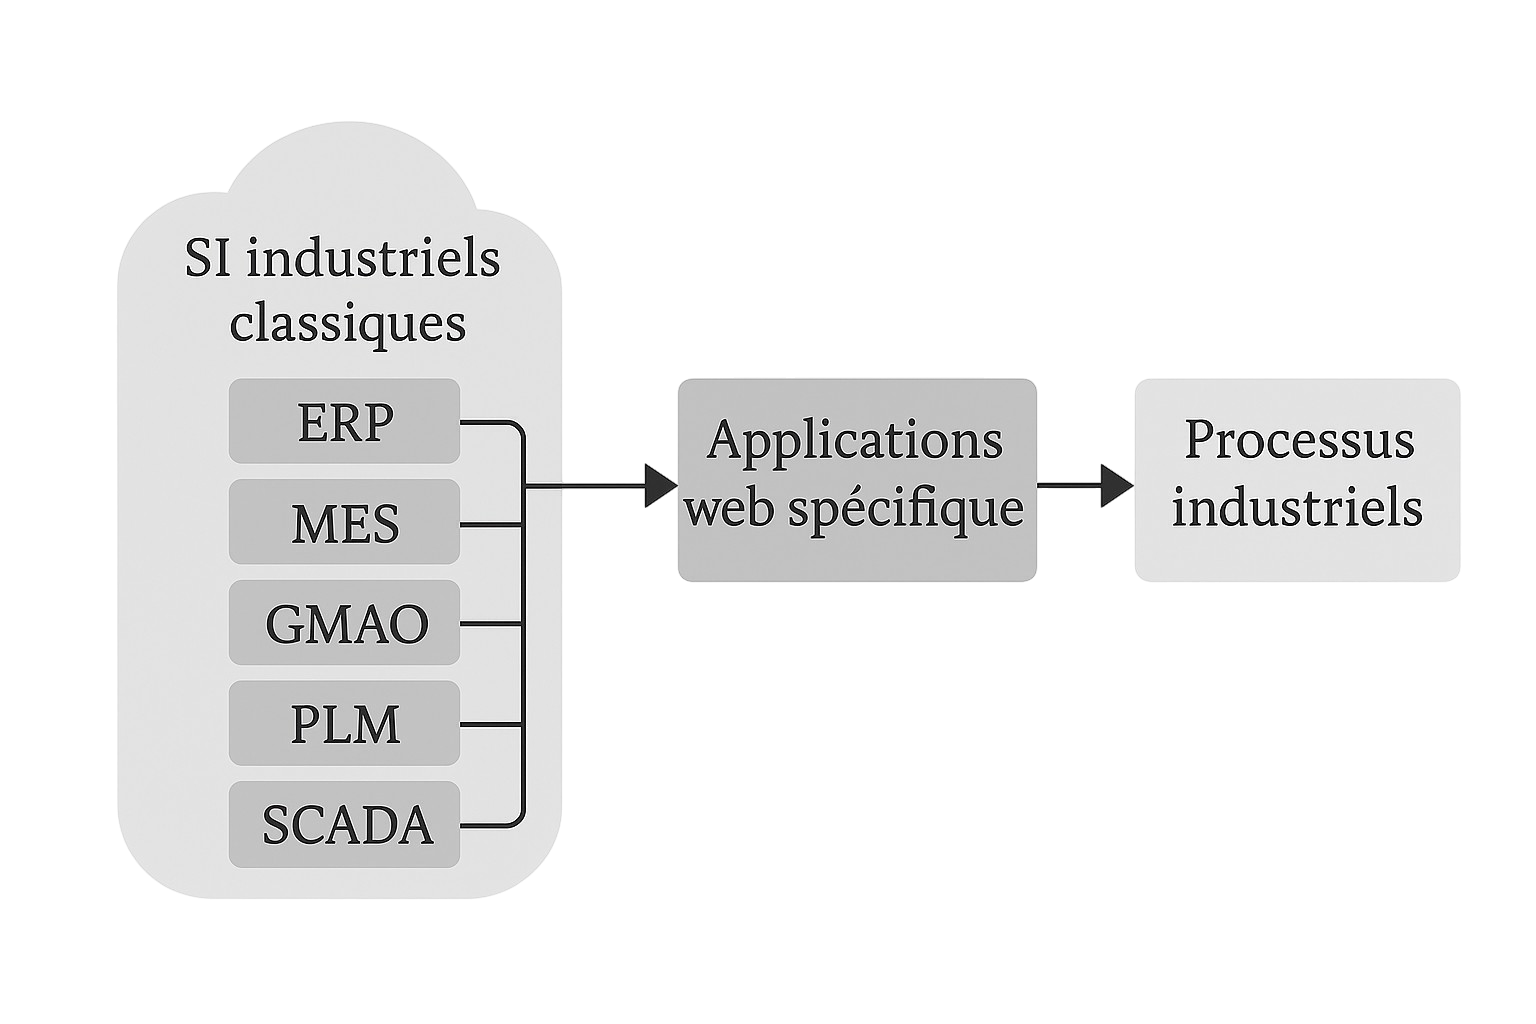
\includegraphics[width=0.8\textwidth]{../Images/app-si.png}
    \caption{Schéma Applications industriels}
\end{figure}

\subsection{Le rôle des applications web sur mesure dans la digitalisation industrielle}

Dans le contexte actuel de transformation numérique, les applications web sur mesure s’imposent comme des leviers incontournables pour répondre aux spécificités et aux exigences opérationnelles des entreprises industrielles.

Les solutions logicielles standards, parmi lesquelles les ERP généralistes ou les tableurs du type Excel, sont souvent par défaut privilégiées. Elles ne peuvent souvent convenir. Or, les applications web, développées sur mesure, permettent la conjugaison agilité, précision métier et expérience utilisateur. Certes, ces outils standardisés peuvent rendre service. À une condition : qu’il s’agisse d’applications transversales. Pour répondre à des processus métiers plus complexes, spécifiques ou évolutifs, leur portée est très limitée.


\vspace{1em}
\textbf{Pourquoi aller au-delà des outils standards ?}  \\

Chaque entreprise industrielle possède une organisation unique, avec ses flux de travail, ses contraintes réglementaires, ses pratiques internes et son vocabulaire technique. Une solution numérique pertinente ne peut donc pas être entièrement générique : elle doit être conçue « à l’image du terrain ». Les applications web sur mesure permettent ainsi de :

\begin{itemize}
    \item \textbf{Répondre à un besoin opérationnel ciblé} \\
    Exemple : suivre des expertises techniques sur des machines tournantes, historiser des contrôles spécifiques, produire des rapports métiers automatisés, etc.

    \item \textbf{Proposer une solution évolutive et progressive} \\
    Contrairement aux gros systèmes rigides, elles peuvent être développées en itérations courtes, testées rapidement, puis enrichies à mesure des retours utilisateurs.

    \item \textbf{S’intégrer au système d’information existant} \\
    Les applications web peuvent consommer des API, interagir avec des bases existantes (SQL, ERP), et s’articuler sans perturber l’écosystème numérique déjà en place.

    \item \textbf{Favoriser l’appropriation par les utilisateurs finaux} \\
    Conçues avec les métiers, les interfaces sont épurées, accessibles sur tablette ou poste industriel, et adaptées aux réalités du terrain.

    \item \textbf{Structurer et fiabiliser les données métier} \\
    Ces applications permettent de capturer l'information là où elle se produit, avec des contrôles qualité intégrés, garantissant la validité et la traçabilité des données remontées.
\end{itemize}


En ce sens, les applications web sur mesure agissent comme des connecteurs intelligents entre le terrain et les systèmes de pilotage stratégique. Elles assurent la continuité numérique entre les opérateurs et les décideurs : en structurant la donnée au moment de sa saisie, elles facilitent son exploitation a posteriori que ce soit pour des audits,la mesure et l'analyse de la performance, ou encore la prise de décision en temps réel.
\\
Plus encore, elles illustrhhhhhhhhhhhhhhhhhhhhhhhhhhhhhhhhhhhhhhhhhhhhhhhhhhhhhhhhhhhhhhent un modèle de numérisation à échelle humaine, où c’est l’outil qui s’adapte à l’utilisateur au lieu de l’inverse. Principe de co-construction et clé du succès des projets de transformation numérique à l’échelle industrielle.


\begin{figure}[H]
    \centering
    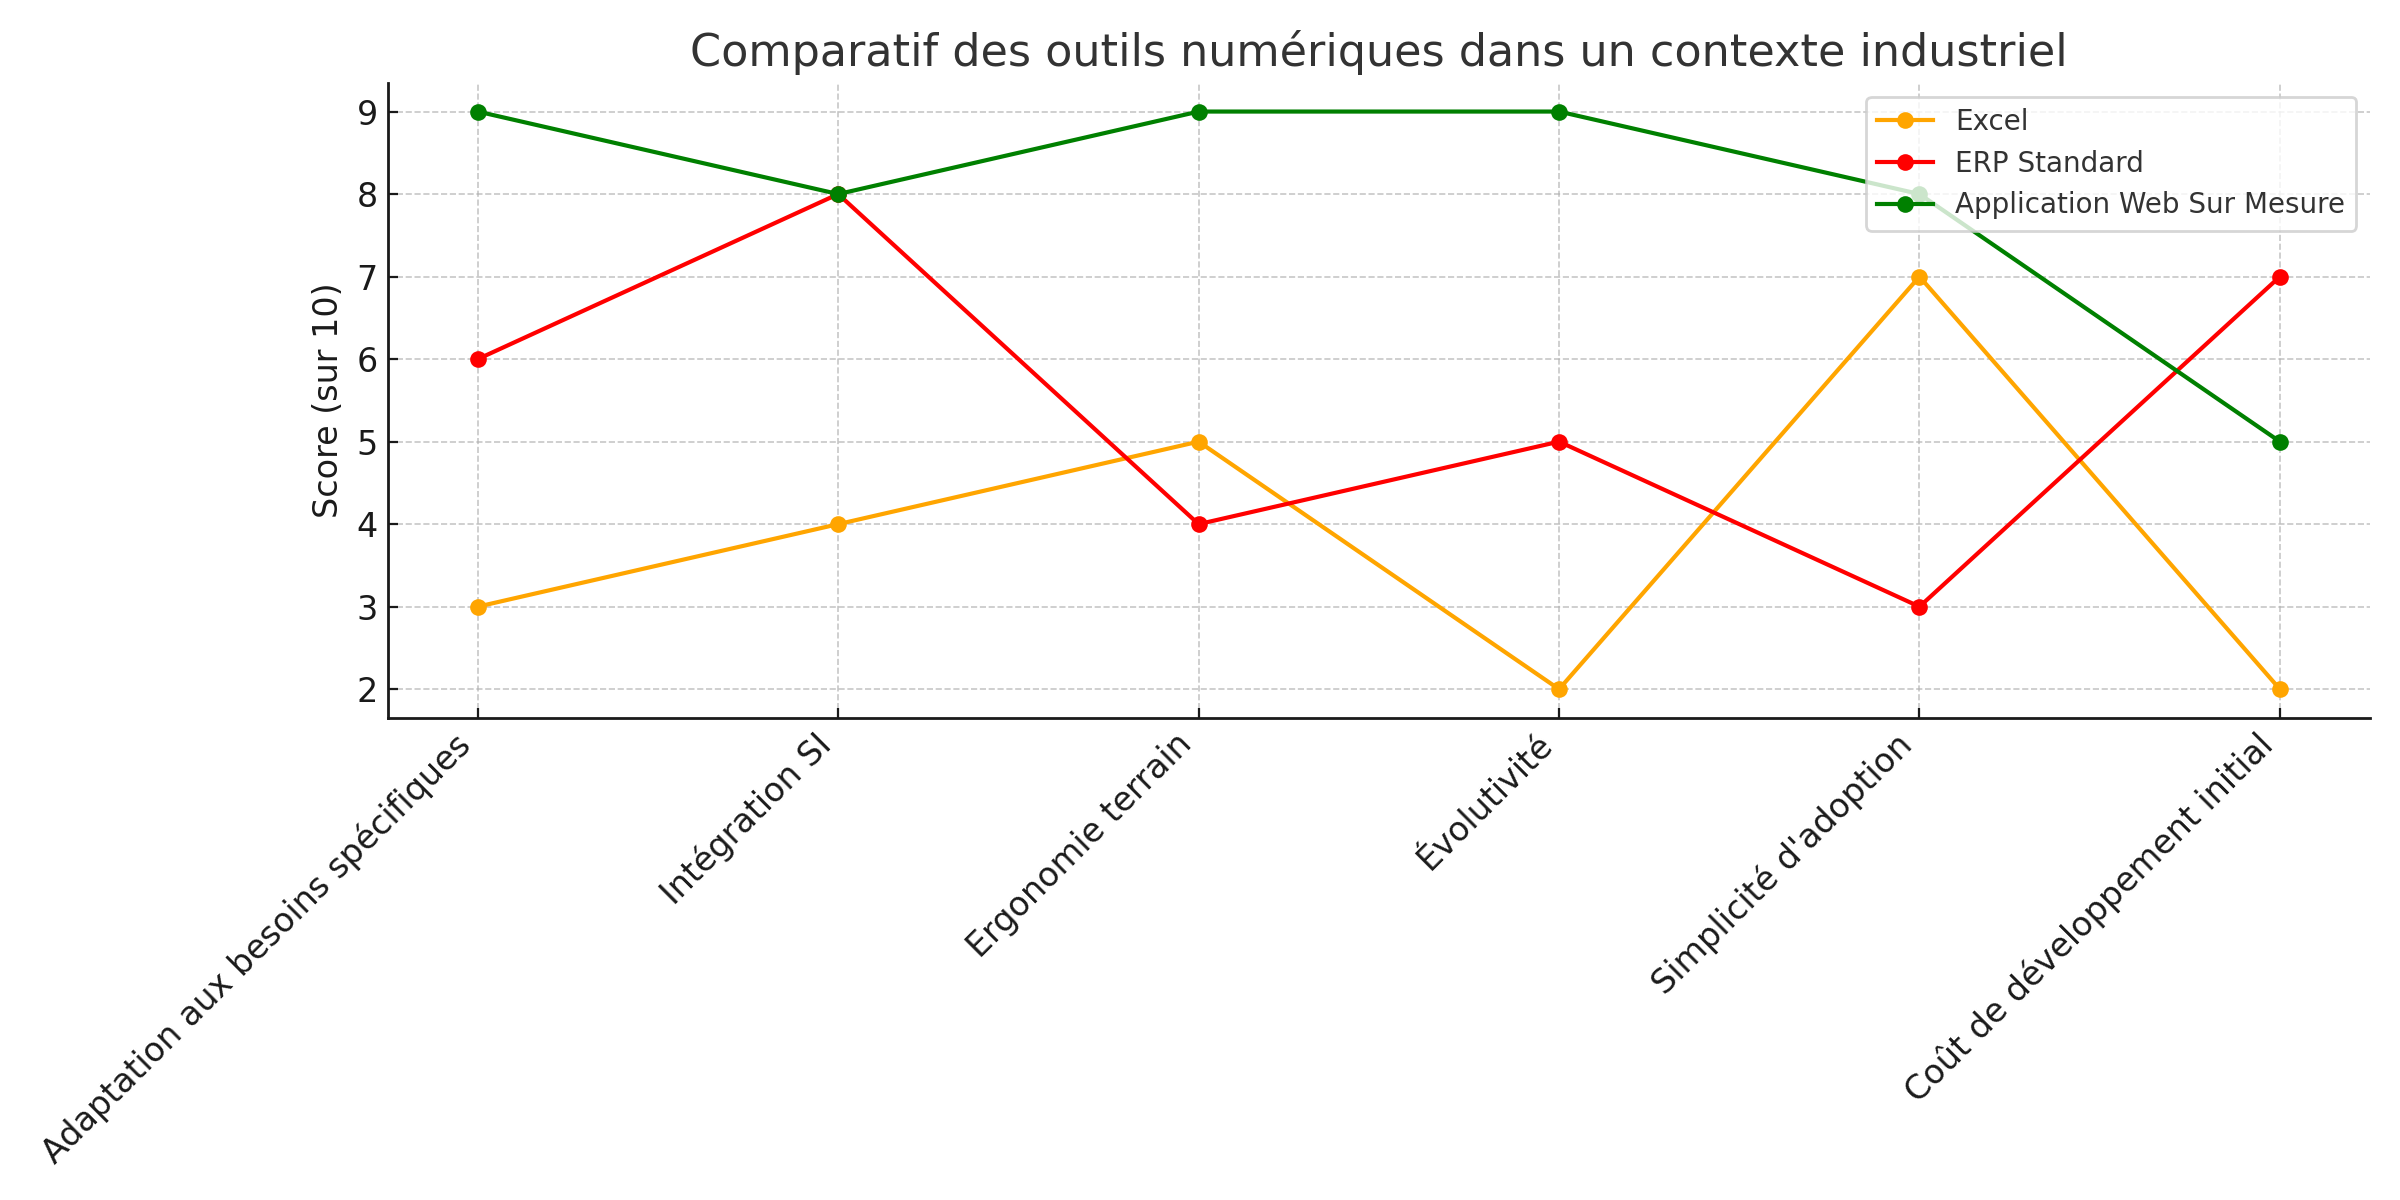
\includegraphics[width=\textwidth]{../Images/app-mesure.png}
    \caption{Schéma comparatif}
\end{figure}

\newpage
\subsection{Limites des outils traditionnels dans l’industrie}

En dépit de la rapide évolution technologique du numérique, un très grand nombre d’entreprises industrielles en particulier des PME et ETI continuent à utiliser tous les jours des outils bureautiques généralistes tels que Microsoft Excel, Word ou Access ou tout simplement des documents papier pour gérer des processus critiques. Ces pratiques émergent parfois d’une tradition bien ancrée, d’un pragmatisme organisationnel ou encore d’un manque de temps ou de moyens pour réaliser une transformation plus ambitieuse.

Cependant, dans un contexte de montée des exigences en matière de traçabilité, de conformité, de qualité et de pilotage en temps réel, ces outils révèlent rapidement leurs limites \cite{bib:industrieavenir, bib:bain2019}.

\begin{itemize}
\item \textbf{Données dispersées et non centralisées}

L’un des problèmes les plus fréquents concerne la dispersion de l’information. Un même processus (ex: expertise d’une machine, suivi budgétaire d’un atelier) peut mobiliser plusieurs fichiers, stockés sur différents postes, partagés par mail ou disponibles sur des serveurs internes sans structuration cohérente. Cela génère :

\begin{itemize}
    \item une perte de temps dans la recherche d’information ;
    \item des doublons non détectés et des versions contradictoires ;
    \item une dépendance aux personnes (savoir où est stocké quoi).
\end{itemize}

\item \textbf{Faible traçabilité des opérations}

Dans l’industrie, la capacité à retracer qui a fait quoi, quand, et dans quel état, est essentielle, notamment pour des raisons de qualité, de responsabilité ou de conformité réglementaire. Les outils bureautiques classiques ne permettent pas de :

\begin{itemize}
    \item historiser proprement les opérations ;
    \item protéger les données contre les modifications non contrôlées ;
    \item suivre les étapes critiques d’un processus métier.
\end{itemize}

Cela expose l’entreprise à des risques lors d’audits ou de litiges.

\item \textbf{Saisie manuelle et erreurs fréquentes}

Les fichiers Excel restent très utilisés pour le suivi de production, la maintenance ou la planification. Pourtant, leur manipulation manuelle :

\begin{itemize}
    \item augmente le risque d’erreur (saisie incorrecte, formules supprimées, cellules mal recopiées) ;
    \item empêche la validation automatique des données (type, cohérence, complétude) ;
    \item rend difficile la consolidation ou l’exploitation des données à grande échelle.
\end{itemize}

\item \textbf{Aucune interconnexion entre services}

L’utilisation d’outils autonomes et non interfacés empêche les services (maintenance, production, qualité, méthodes, direction) de partager une vision commune. On observe souvent :

\begin{itemize}
    \item des saisies redondantes d’une même information ;
    \item des ruptures de communication entre phases (ex: expertise, rédaction de rapport et archivage) ;
    \item une perte d’efficacité globale sur l’ensemble de la chaîne.
\end{itemize}

\item \textbf{Manque de pilotage temps réel}

Avec les outils classiques, la remontée des informations est lente, parfois hebdomadaire voire mensuelle. Il devient impossible de :

\begin{itemize}
    \item suivre l’évolution d’un projet en temps réel ;
    \item réagir rapidement à un dépassement budgétaire ou à une dérive qualité ;
    \item construire des tableaux de bord fiables à jour quotidiennement.
\end{itemize}

\item \textbf{Charge mentale pour les équipes terrain}

Les techniciens, chefs d’équipe ou responsables doivent souvent jongler entre plusieurs fichiers, dossiers partagés, impressions papier, et mails informels. Cela génère :

\begin{itemize}
    \item une surcharge administrative inutile ;
    \item un éloignement de leur cœur de métier (diagnostic, fabrication, intervention) ;
    \item un rejet progressif des outils numériques, perçus comme lourds et mal conçus.
\end{itemize}

\item \textbf{Manque d’adaptabilité aux évolutions}

Enfin, les outils bureautiques traditionnels sont difficilement adaptables. Ajouter une fonctionnalité, automatiser une tâche, ou ajuster un workflow nécessite souvent des manipulations complexes, qui dépendent de compétences spécifiques, rarement disponibles en interne.

\end{itemize}
\subsection{Contexte chez Jeumont Electric}

Chez Jeumont Electric, plus particulièrement sur le site de Carquefou, la transformation numérique n’est pas de la logique d’une tendance à suivre pour une mode technologique. Mais bien une réponse immédiate à une série de problèmes réels rencontrés sur le terrain par les équipes opérationnelles et empêchant parfois la performance de l’entreprise. Des problèmes, que l’on a longtemps perçus comme tolérables au nom du pragmatisme ou de la routine, et qui ont montré progressivement leurs effets négatifs sur la productivité, la qualité, la traçabilité et la fluidité des processus internes.

\subsubsection{Outils existants}

Avant le démarrage de la mission, les processus métiers de plusieurs services clés notamment la maintenance, l’expertise technique et la production reposaient sur des outils de gestion anciennes. Il s’agissait principalement de :

\begin{itemize}
    \item fichiers Excel utilisés comme bases de suivi ou de calcul, souvent stockés localement sur les postes de travail ou partagés via les serveurs internes ;
    \item rapports papier renseignés manuellement en atelier, puis scannés et stockés sans classification systématique ;
    \item e-mails et discussions orales pour transmettre des consignes ou des informations techniques ;
    \item anciens outils internes développés il y a plusieurs années avec des technologies désormais obsolètes.
\end{itemize}

Ces pratiques, héritées d’une organisation historique orientée terrain plus que numérique, permettaient certes de faire fonctionner les opérations, mais elles posaient plusieurs limites dès que l’on cherchait à fiabiliser, centraliser, tracer ou piloter les informations de manière plus structurée.

\begin{enumerate}
\item \textbf{Conséquences directes sur le fonctionnement}

Les équipes faisaient régulièrement état de difficultés rencontrées au quotidien, notamment :

\begin{itemize}
    \item une perte de temps importante dans la recherche d’informations techniques ou budgétaires ;
    \item une traçabilité ou suivi incomplète ou incohérente des opérations réalisées ;
    \item une surcharge administrative pour les techniciens et opérateurs ;
    \item un manque de visibilité en temps réel pour les chefs de projet ;
    \item une hétérogénéité des pratiques d’un service à l’autre, générant des écarts de qualité.
\end{itemize}

Ces contraintes impactaient directement la qualité du travail, la réactivité face aux urgences, la capacité à répondre aux audits clients, et la fluidité globale des échanges.

\item \textbf{Un besoin d’outils plus adaptés aux réalités métier}

Face à ces constats récurrents, la direction du site de Carquefou a initié une réflexion sur la modernisation des outils internes. Plutôt que d’adopter un progiciel lourd ou un ERP global, l’entreprise a fait le choix stratégique de développer des \textbf{applications web sur mesure}.

\newpage
Ce choix repose sur plusieurs critères :

\begin{itemize}
    \item souplesse des technologies web pour adapter les interfaces aux contraintes métier ;
    \item rapidité de développement et de déploiement ;
    \item accessibilité via navigateur sans installation complexe ;
    \item centralisation des données et sécurisation des accès par rôles ;
    \item réduction des ressaisies et erreurs grâce aux contrôles automatiques ;
    \item génération automatique de rapports et indicateurs utiles.
\end{itemize}

\item \textbf{Un engagement progressif mais structuré}

La mission confiée dans le cadre de cette alternance s’inscrit dans cette stratégie. Jeumont Electric a fait le choix d’une approche \textbf{progressive, pragmatique et orientée terrain}, en sélectionnant trois axes d’amélioration jugés prioritaires :

\begin{enumerate}
    \item \textbf{Une base d’expertise} pour centraliser, partager, valider et archiver les résultats des expertises électriques et mécaniques.
    \item \textbf{Une application de traçabilité des barres}  pour suivre la fabrication et l’intégration des enroulements, étape par étape au cours de la fabrication, avec un suivi de la qualité et de la performance.
    \item \textbf{Une application de suivi budgétaire de la maintenance} pour améliorer le pilotage financier des interventions du service de maintenance du site de Carquefou.
\end{enumerate}


\begin{figure}[H]
    \centering
    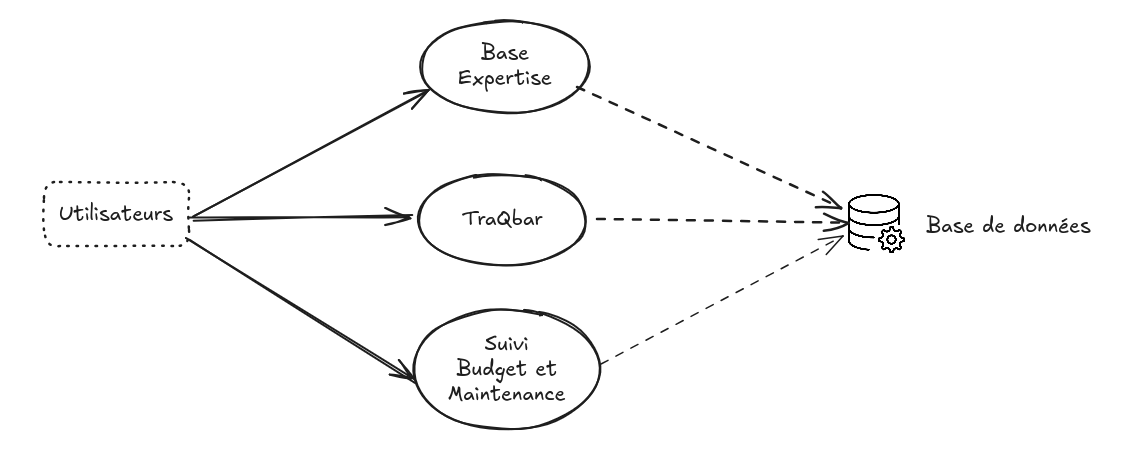
\includegraphics[width=\textwidth]{../Images/application-web.png}
    \caption{Applications web réalisées }
\end{figure}

Chaque projet a été conçu en lien étroit avec les utilisateurs finaux, à travers une démarche de co-conception impliquant des ateliers de recueil des besoins, des tests en situation réelle, et des ajustements itératifs.

Cette démarche, en cohérence avec les principes du développement Agile, constitue un modèle reproductible pour toute entreprise industrielle cherchant à moderniser ses outils sans bouleverser son organisation.

\end{enumerate}



\subsection{Conclusion}

Les limites constatées sur le site de Carquefou, des outils usuellement utilisés il y a encore peu de temps nous ont conduits à identifier un besoin évident en matière de modernisation et c’est la digitalisation par le biais du développement d’applications web sur mesure qui est apparue comme la réponse pertinente, ciblée et progressive. Dans le chapitre suivant est présentée la mission concrète qui a permis de participer à cette transition.



\newpage
\section{Contexte et enjeux de la mission}
\subsection{Cadrage de la mission}

Cette mission d'alternance s’inscrit dans le cadre d’une stratégie de digitalisation progressive menée sur le site de Carquefou de Jeumont Electric. Elle visait à moderniser des processus industriels identifiés comme critiques, notamment la gestion des expertises techniques, la traçabilité des barres Roebel, et le suivi budgétaire des dépenses de maintenance. L’objectif était double : renforcer l’efficacité opérationnelle tout en favorisant l’adoption de nouveaux outils numériques par les équipes terrain.

\subsubsection{Origine du projet}

Plusieurs services (maintenance, production, projets), ont exprimé un constat partagé sur les limites de solutions classiques (Excel, papier, solutions locales) : pas de traçabilité centralisée, double saisie, pas de réactivité en cas de non-conformité. Ces constats justifiaient la réalisation d’une solution numérique bien ciblée.

Les chefs de service, les techniciens de terrain et les chefs de projets se heurtaient à des difficultés tant sur la saisie, que sur la consolidation et l’exploitation des données. Cela se traduisait par un manque de réactivité, une qualité documentaire parfois insuffisante, ou une incapacité à satisfaire les clients ou dans le cadre d’audits internes.

Dans ce contexte, l'entreprise a exprimé le besoins de créer des outils numériques  fait sur mesure, qui répondraient d'une maniére précise aux problèmes du travail vécus, tout en s'intégrants aux pratiques sur terrain. Le périmètre de la mission a donc été fixé autour d'un point clé: digitaliser trois processus industriels critiques à l'aide de l'application web conçues spécifiquelment pour le site de Carquefou.

\subsubsection{Définition du périmètre}

Trois besoins ont été identifiés comme prioritaires :

\begin{enumerate}
    \item \textbf{Centralisation des expertises techniques} : les interventions électriques et mécaniques menées sur les équipements industriels donnaient lieu à des relevés et rapports expertise et final, souvent dispersés ou stockés sur un serveur de fichiers. Il s’agissait de structurer ces données dans une base d’expertise numérique, exploitable, sécurisée et génératrice de rapports standardisés.

    \item \textbf{Traçabilité des barres Roebel} : Pour ce qui concerne la fabrication des barres utilisées dans les enroulements des stators, un suivi rigoureux est indispensable. Le processus utilisé était fondé sur une base de donnée ancienne qui ne correspondait plus aux besoins actuels. Le besoin était de créer une application plus récente, correspondant à de nouveaux besoins apparus suite à la réorganisation des postes de fabrication des barres. 

    \item \textbf{Suivi budgétaire de la maintenance} : les coûts liés aux interventions n’étaient pas suivies en temps réel. Le chef de service maintenance devait compiler des éléments collectés à partir de plusieurs sources, en l’occurrence sous la forme d’un fichier excel afin de reconstituer les dépenses. L’objectif est de leur permettre de disposer d’un outil leur permettant d’avoir une vision budgétaire actualisé, clair et filtrable par type d’intervention, machine ou période.
\end{enumerate}

Chacune de ces problématiques représentait un maillon stratégique dans le fonctionnement global du site. L’idée n’était pas de remplacer les systèmes informatiques existants à grande échelle, mais d'ajouter d'autres outils, interconnectés, orientés usage, et capables d’apporter un bénéfice immédiate.

\subsubsection{Nature de la mission}
La mission confiée dans le cadre de cette alternance ne se limitait pas à la simple réalisation technique d’un logiciel. Elle faisait également partie d’un ensemble plus vaste de transformation numérique, en relation directe avec les objectifs stratégiques du site de Carquefou. Caractérisée par son caractère transversal, elle a mobilisé des compétences diverses et variées : informatique, analyse fonctionnelle, gestion de projet, conduite du changement, communication sur le projet avec l’ensemble des parties prenantes.

Elle s'est articulée autour de plusieurs volets clés:


\begin{itemize}

    \item \textbf{Analyse des besoins} : recueil des attentes des utilisateurs via des entretiens, des observations sur le terrain, et des documents existants comme les cahiers des charges
    
    \item \textbf{Modélisation des processus actuels} : cartographie des workows, identification des points de blocage, des étapes critiques et des données manipulées.
       
    \item \textbf{Conception des solutions} : définition de l'architecture applicative, conception des interfaces, choix technologiques ( Symfony, MySQL, TWIG, Javascript etc..)
    
    \item \textbf{Développement incrémental} :mise en oeuvre des fonctionnalités par lots par d'application, avec des livraisons régulières pour validation intermédiaire.
    
    \item \textbf{Tests fonctionnels et recette utilisateur} : mise en situation réelle dans l'atelier ou au bureau, collecte des retours et ajustements.
    
    \item \textbf{Déploiement et accompagnement} : mise en production sur le réseau de l’entreprise, rédaction de guides, formation des utilisateurs, et support initial.
\end{itemize}

\subsubsection{Positionnement dans l’entreprise}

Le projet a été réalisé en étroite co-construction avec les équipes métiers de Jeumont Electric, ateliers, maintenance, production, et chefs de projets, afin de prendre en compte la réalité opérationnelle des projets, en comprenant les contraintes, les priorités, les habitudes de chaque service. Pour co-construire de façon pragmatique les solutions en lien avec les utilisateurs finaux et garantir une bonne adéquation de l’outil au besoin des utilisateurs, les échanges ont été réguliers, limitant le risque de dérives fonctionnelles ou de déconnexion entre le fonctionnement de l’outil et l’utilisation qui en sera faite.

La mission était orchestrée par les tuteurs de l’entreprise, qui avaient la responsabilité du pilotage global et du respect des orientations stratégiques de l’entreprise. Dans le cadre d’arbitrages fonctionnels associés prenant en compte les besoins exprimés et les ressources disponibles dans le cadre des standards internes de sécurité informatique, d’accessibilité réseau ou de conformité documentaire.

Un des principaux atouts du projet résidait dans ses modalités de réalisation : le développement des applications a été assuré en interne, dans le cadre de l’alternance, favorisant ainsi une forte réactivité aux retours utilisateurs. Il s’est agi de postures Agiles, associant cycles courts de tests, itérations rapides et capacité d’adaptation à des contraintes évolutives, alors qu’une solution sous-traitée aurait pu nuire à l’appropriation des outils par des utilisateurs et à la cohérence entre choix techniques et attentes métier.

\subsubsection{Un projet à impact local mais à potentiel global}

Bien qu’originellement circonscrit au site de Carquefou, le projet portait en réalité une ambition bien plus large telle qu’un démonstrateur à échelle humaine visant à valider une approche pragmatique, itérative et ancrée sur le terrain d’une digitalisation ne s’inscrivant pas seulement dans la résolution d’irritants opérationnels locaux mais à poser les fondements d’une méthodologie empruntant à la reproductibilité pouvant inspirer d’autres projets numériques chez Jeumont Electric.

En s’appuyant sur des technologies web modernes, des processus de co-conception Agile et une proximité avec les utilisateurs finaux, le projet a livré des outils simples, robustes et utiles immédiatement. Cette efficacité associée à la maitrise de ses coûts de développement (parce que conduits en interne dans le cadre de l’alternance), a suscité un grand intérêt auprès d’autres services.

De fait, les solutions mises en œuvre, base d’expertise, suivi de production, pilotage budgétaire, peuvent être déclinées ou adaptées à d’autres entités du groupe, avec des ajustements minimes. Leur modularité, leur compatibilité avec les infrastructures existantes et leur architecture orientée métier en font des briques logicielles prometteuses pour une montée en puissance progressive.

Ce projet, tout en restant modeste dans sa taille, démontre qu’il est possible d’engager une transformation numérique industrielle sans bouleverser les structures existantes, à condition de partir des besoins du terrain et d’impliquer les équipes dès la conception.

\subsection{Objectifs de la mission}

La mission qui m’était assignée dans le cadre de cet contrat d'alternance dépassait le cadre d’une simple action technique. Elle se plaçait dans une ambition stratégique de pérennisation d’un meilleur fonctionnement de processus industriels jugés critiques pour l’entreprise. Il ne s’agissait donc pas de concevoir ou mettre en place simplement une solution logicielle, mais de contribuer à une transformation plus profonde, impliquant à la fois des aspects technologiques, organisationnels et humains.

Le principal défi du projet se trouvait bien dans le fait d’implémenter des outils numériques tout en les rendant accessibles aux utilisateurs finaux, ce qui n’allait pas sans engendrer un travail préalable de compréhension de leurs besoins, de leurs pratiques, et de leurs résistances au changement. L’accompagnement à la transformation se naturel à l’ensemble des tâches sur les solutions, comme constitutif, au même titre que les développements des solutions.

Dès les premières phases du projet, trois catégories d’objectifs étaient explicitement identifiés afin de matérialiser le travail et assurer la cohérence du projet :

\subsubsection{Objectifs techniques}

Dans le cadre de cette mission, le cahier des charges technique stipule que les solutions numériques à développer devront être robustes, sécurisées, mais aussi et surtout facilement maintenables sur le long terme. Il ne s’agit donc pas seulement de développer une « application » qui soit fonctionnelle ou au moins utilisable par les utilisateurs finaux, mais de proposer des outils intégrés au contexte de l’entreprise, à l’environnement informatique existant, en conformité avec les spécifications internes. Plusieurs points clés étaient à prendre en considération :

\begin{itemize}
    \item \textbf{Développer des applications web accessibles et performantes}, utilisables directement dans un navigateur, sans installation sur un poste local, permettant ainsi à la fois d simplifier le déploiement, d’assurer un accès uniforme et de garantir une compatibilité optimale avec le parc informatique existant, à savoir, les équipements déjà en action dans l’entreprise.
    
    \item \textbf{Organiser les données dans une base de donnéees MySQL sécurisée}, afin de permettre une saisie fiable, un accès rapide à l’information, et la possibilité de faire des analyses ou d’en extraire des rapports facilement. L’objectif était d’éviter les erreurs de manipulation tout en facilitant l’exploitation des données.
    \item \textbf{Mettre en œuvre les règles de sécurité de l’entreprise}, par le biais de processus d’identification, de gestion des droits d’accès, et une pleine traçabilité des opérations délicates. Ces prémisses étaient vraies pour garantir la sécurité des données, et le respect des politiques internes.
    
    \item \textbf{Assurer la compatibilité avec les outils déjà utilisés}, comme les serveurs de fichiers partagés ou d’autres systèmes internes. Le but était d’éviter des interconnexions complexes tout en gardant une bonne communication entre les outils.
    
    \item \textbf{Documenter clairement tout le travail réalisé}, aussi bien le code que l’architecture générale. Cette documentation avait pour but de faciliter la prise en main par d’autres développeurs ou équipes internes, en vue de maintenir ou de faire évoluer la solution par la suite.


\end{itemize}

\subsubsection{Objectifs fonctionnels}
Les objectifs fonctionnels de la mission s’attaquaient aux besoins réels des utilisateurs et à la constriction apportée par les outils antérieurs. Il s’agissait de construire des solutions qui soient véritablement efficaces au-delà de leur seule pertinence théorique et qui soient réellement utiles afin qu’elles soient simples d’accès et effectivement appropriées par les équipes.

Pour cela plusieurs axes d'améliorations avaient été identidiés des l'amont :

\begin{itemize}
    \item Limitation des erreurs de saisie et des doublons par la construction de formulaires bien structurés avec des champs contrôlés, des parcours guidés permettant de fiabiliser l’enregistrement des données.
    
    \item Traçabilité de l’ensemble des actes par l’enregistrement systématique de chaque acte (création, modification, validation…) d’informations telles que la date, l’auteur et le contexte dans lequel il a été réalisé.
    
    \item Automatisation des tâches répétitives, notamment dans la production des rapports et certains calculs récurrents (budgets, synthèses d’activité, …) afin de faire gagner du temps tout en diminuant la part d’erreurs à un moment donné du processus d’enregistrement.
    
    \item Proposer des outils d'analyse simples et accessibles, sous forme de tableaux de bord clairs, pour permettre un suivi en temps réel de certains indicateurs, qu'ils soient techniques ou financiers.
	\item Adapter l'interface aux usages réels des utilisateurs, en particulier pour les techniciens en atelier. L'objectif était de proposer une navigation rapide, avec une ergonomie pensée pour les écrans de bureau, afin de ne pas ralentir leur travail.    
        
\end{itemize}

\subsubsection{Objectifs humains et organisationnels}

Dans un cadre industriel, un projet numérique ne se conclut par un succès que si on prend en compte la dimension humaine. Un outil peut être techniquement avancé, mais il ne s’avérera véritablement utile que si ceux qui s’en servent au quotidien s’en emparent. C’est donc tout naturellement que les enjeux humains et organisationnels ont été au cœur de cette mission.

Des objectifs opérationnels ont été fixés afin de déclencher l’adhésion, l’appropriation et l’utilisation pérenne des outils développés :

\begin{itemize}
    \item Impliquer les utilisateurs finaux de façon systématique dès le lancement du projet : c’est concrétisé par des entretiens réguliers, des maquettes à valider ensemble, des tests sur le terrain. La démarche participative ainsi engagée a permis d’affiner leurs attentes et de concevoir un outil en phase avec leur quotidien.

    \item Alléger la charge administrative des équipes, en automatisant certaines tâches et en supprimant les ressaisies inutiles, pour leur faire gagner du temps et réduire la pénibilité de certaines opérations répétitives ou peu productives.
    
    \item Accompagner la prise en main des outils, grâce à une montée en compétence progressive. Des formations ciblées, des supports clairs et une assistance au démarrage ont été mises en place pour que chacun puisse se sentir à l’aise avec les nouveaux usages.
    
    
    \item Ajuster les pratiques et les mentalités, en montrant que la digitalisation peut être un vrai levier d’amélioration et non un élément supplémentaire de complexité du travail. L’idée étant de créer un climat de confiance autour du changement.
    
    \item Anticiper l’extension possible du projet, en gardant à l’esprit que les solutions mises au point doivent être réutilisables par d’autres équipes, d’autres processus, voire d’autres sites. Il s’agissait aussi de poser les bases d’un modèle reproductible.
    
\end{itemize}

\begin{figure}[H]
  \centering
  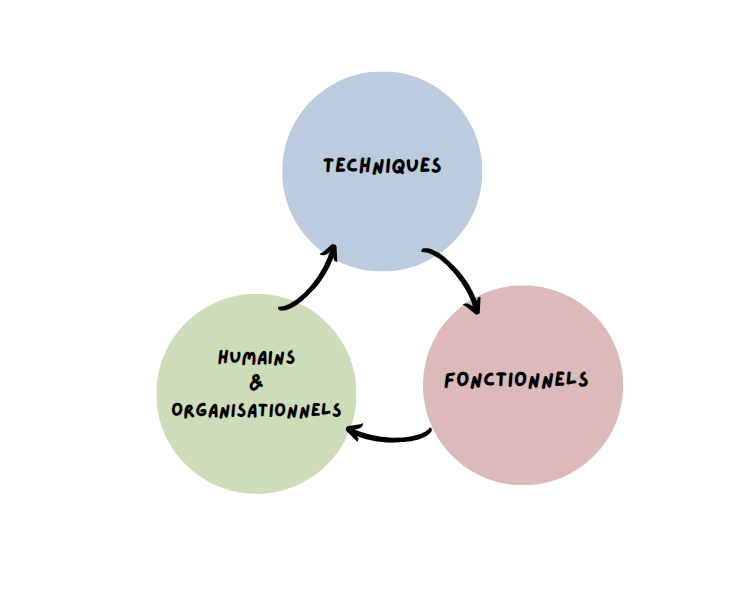
\includegraphics[width=0.9\textwidth]{../Images/objectis.png}
  \caption{Objectifs de la mision}
\end{figure}

Ces objectifs techniques, fonctionnels et humains ont guidé l’ensemble du projet, du cadrage initial jusqu’à la mise en production. À chaque étape, ils ont servi de repères pour orienter les choix techniques, valider les fonctionnalités livrées et structurer l’organisation du travail, notamment dans une démarche Agile. Plus qu’un simple développement applicatif, cette mission visait à initier une dynamique d’amélioration durable, en apportant aux équipes de Jeumont Electric des outils concrets, pensés pour leur quotidien, et porteurs de valeur sur le long terme.

\subsection{Contraintes techniques et organisationnelles}

La réalisation de cette mission ne s’est pas déroulée dans un environnement neutre, dénué d’enjeux. Elle a joué un rôle à prendre en compte (à composer) avec un certain nombre de contraintes (techniques, organisationnelles) qui ont influencé autant les choix de conception, que les priorités fonctionnelles, que le rythme d’avancement. Identifier ces contraintes au tout départ et les intégrer dans la démarche globale d’accompagnement au changement a été la condition pour garantir la faisabilité du projet, la robustesse des solutions mises en place et leur appropriation par les utilisateurs.


\subsubsection{Contraintes techniques}

\begin{itemize}
    \item \textbf{Infrastructure informatique existante} : le développement se veut basé sur l’infrastructure informatique interne de Jeumont Electric, sans recourir à des solutions cloud externes. Le déploiement se doit donc être localisé (intranet) et compatible avec les navigateurs et systèmes d’exploitation disponibles.

    \item \textbf{Connexion réseau limitée dans certaines zones} :  notamment dans les ateliers, où certaines machines sont éloignées des points d’accès réseau. Les applications devront être légères et robustes pour fonctionner dans un environnement réseau parfois instable.

    \item \textbf{Sécurité et accès} : il faut restreindre l’accès aux données sensibles (historique d’interventions, rapports d’expertise, budgets) en réalisant une gestion fine des droits utilisateurs, avec des niveaux d’accès différents selon les rôles.
    
    \item \textbf{Interopérabilité} : même si l’on n’est pas là pour remplacer l’ERP ou les outils existants, on doit veiller à une certaine compatibilité dans les formats de données pour permettre une réutilisation future ou une extension fonctionnelle.

    \item \textbf{Temps de développement limité} : la mission se déroulant en alternance, il faut faire des choix réalistes vis à vis du périmètre fonctionnel : privilégier une approche incrémentale et testable.
\end{itemize}

\newpage
\subsubsection{Contraintes organisationnelles}

\begin{itemize}
    \item \textbf{Disponibilité des utilisateurs} :les techniciens, chefs d’atelier ou responsables de service ont peu de disponibilités pour des réunions longues ou des ateliers de conception. Il a donc fallu proposer des formats courts, des démonstrations directes sur le terrain, et avancer plutôt par ajustements successifs.
    
    
    \item \textbf{Hétérogénéité des pratiques} : certains processus n’étaient pas formalisés ou variaient selon les équipes. Avant de digitaliser, il a parfois fallu harmoniser les pratiques existantes, ou du moins documenter les écarts pour que les outils restent compatibles avec la réalité du terrain.

    \item \textbf{Culture numérique variable} :  tous les utilisateurs n’avaient pas la même aisance avec les outils informatiques. On a dû adapter l’ergonomie des interfaces, prévoir une phase de prise en main accompagnée, et construire des outils simples, intuitifs, et accessibles.

    \item \textbf{Respect des priorités opérationnelles} : la mission devait s’insérer dans un quotidien déjà chargé. Tests, échanges, déploiements étaient donc prévus pour se faire sans perturber les opérations encours, aux pics d’activité ou sur des périodes sensibles (audits, fin de mois etc ...).
    
    \item \textbf{Évolutivité et maintenance} : l’entreprise souhaitait conserver une capacité future à faire évoluer les outils. Il a donc fallu documenter proprement le code, structurer les bases de données de manière modulaire, et préparer un transfert de compétences pour l’après-projet.
\end{itemize}

L’identification et la prise en compte de ces différentes contraintes ont fondamentalement contribué à construire un projet réaliste, pertinent, et accepté par les parties prenantes, prévenant les écueils classiques des projets numériques industriels, à savoir la sur-spécification, le rejet de l’utilisateur ou l’incompatibilité technique. Elles ont été intégrées dès la phase de planification initiale, permettant de prévoir les risques liés à l’absence de documentation ou à la variabilité dans les pratiques.


\subsection{Attentes de l’entreprise}
Derrière la mission confiée dans le cadre de cette alternance, Jeumont Electric avait des attentes explicites formulées par la direction technique, par les responsables opérationnels ou par les utilisateurs finaux. L’enjeu dépassait tout bonnement le développement d’un nouvel outil numérique : il s’agissait de poser les fondements d’une transformation durable, visible et effective, des pratiques de l’entreprise.

\subsubsection{Attentes à court terme}

À court terme, Jeumont Electric attendait de la mission des résultats tangibles, visibles et directement utilisables sur le terrain. L’objectif n’était pas juste de rendre un prototype ou un proof of concept, mais d’apporter des améliorations immédiates à certains processus clé. Cinq attentes majeures structuraient la mission :

\begin{itemize}
	\item \textbf{Améliorer le quotidien des utilisateurs  }
\end{itemize}
Les premiers impactés par les évolutions numériques sont les équipes opérationnelles. La charge administrative pesait particulièrement sur les techniciens et les responsables de service, notamment la répétition induite par certaines tâches (saisies multiples, rapports manuels, classements de documents). Il convenait donc de simplifier leurs routines en automatisant certains traitements, en normalisant des formats de saisie, en supprimant les ressaisies. Cela devait permettre de mieux les soulager, de leur faire gagner du temps, mais aussi de réduire certains risques liés à l’erreur ou à la perte d’information.

\begin{itemize}
\item \textbf{Centraliser les données critiques  } \
\end{itemize}

Avant le projet, les informations étaient le plus souvent éparpillées sur des fichiers Excel partagés d’un côté ou circulait par e-mail de l’autre ; quant à certaines données, elles étaient renseignées directement dans le serveur fichiers de l’entreprise. Cette fragmentation gênait l’accès, la mise à jour ou la sécurisation des données. Il était donc nécessaire de concevoir une solution centralisatrice réunissant au sein d’une même interface toutes les données techniques, financières et logistiques. Une centralisation assurait également la fiabilité des analyses et la fluidité des échanges entre services.

\begin{itemize}
\item \textbf{Renforcer la fiabilité documentaire } \
\end{itemize}

Dans un contexte industriel, la qualité de la documentation est un enjeu majeur tant pour les audits internes et les contrôles qualité que pour les relations avec les clients. L’objectif était ensuite de permettre la génération automatique de rapports complets, structurés selon des formats validés, et conformes à des exigences réglementaires ou contractuelles. Cette automatisation devait réduire les oublis et garantir l’homogénéité des documents produits tout en facilitant leur exploitation a posteriori.

\begin{itemize}
\item \textbf{Expérimenter une approche Agile  } \
\end{itemize}

La direction technique souhaite tester une méthode de développement plus souple et réactive, fondée sur des cycles courts, des retours utilisateurs fréquents, une adaptation permanente. L’« Agile », approche alternative, est une rupture avec des pratiques plus traditionnelles reposant sur des cahiers des charges rigides. L’alternance constituait un contexte idéal pour expérimenter cette démarche, en co-construisant les outils au fur et à mesure, avec des phases de tests et d’ajustements rapides.

\newpage
\begin{itemize}
\item \textbf{Permettre un déploiement rapide  } 
\end{itemize}

Pour conclure, l’un des enjeux centraux résidait dans l’obtention rapide d’une version au moins utilisable, l’entreprise vise l’exploitation des résultats de la mission à l’issue d’une période d’alternance, sans devoir passer par un long programme d’intégration ou un lourd plan de formation, en ayant à disposition des interfaces intuitives, exploitables, suffisamment solides pour une mise en production même si certaines fonctionnalités devaient être complétées plus tardivement.
\subsubsection{Attentes à moyen et long terme}

Au-delà des objectifs opérationnels immédiats, la mission confiée s’inscrivait dans une vision plus large portée par Jeumont Electric : celle d’une transformation progressive et maîtrisée de ses pratiques industrielles à travers le numérique. L’ambition n’était pas seulement de résoudre un problème local, mais bien d’explorer un nouveau modèle de développement digital, reproductible et évolutif. Les attentes à moyen et long terme reflètent cette volonté stratégique. 

\begin{itemize}
 \item \textbf{Structurer une base de savoir-faire numérique}
\end{itemize}
L’un des enjeux majeurs recensés par l’entreprise a donc consisté dans la préservation et la valorisation de l’expertise interne. En effet, au fil des années, Jeumont Electric s’est constitué un très important bagage de connaissances techniques et opérationnelles, le plus souvent conservées sous forme de documents isolés, de fichiers locaux ou de pratiques informelles. La digitalisation devait permettre de rendre ce savoir formalisé accessible à tous tout en le protégeant des risques de perte liés aux mobilités internes, aux départs à la retraite ou à la réorganisation des équipes : l’outil développé devait donc être le référentiel vivant structurant la mémoire technique de l’entreprise.
    
    
\begin{itemize}
   \item \textbf{Renforcer la transversalité entre services}
\end{itemize}
Dans un environnement industriel où plusieurs métiers interagissent en continu, la circulation fluide de l’information est un facteur clé d’efficacité. Une autre attente forte de l’entreprise était donc de favoriser la transversalité entre les services – production, maintenance, logistique, qualité, direction – en leur offrant une plateforme commune. Cette base partagée devait faciliter la coordination, limiter les silos d’information, et permettre un suivi global des activités.

\begin{itemize}
    \item \textbf{Accroître la culture numérique de l’atelier}
\end{itemize}
   Jeumont Electric voulait aussi être le moteur d’un changement culturel à l’intérieur de l’entreprise, amené à faire prendre conscience à ses équipes de terrain de la pertinence des outils numériques. Il s’agissait, non pas de rompre brutalement avec les méthodes de travail en place, mais d’amener les pratiques à évoluer progressivement, en développant des solutions intuitives, pertinentes et souples, respectant les spécificités et les contraintes de travail des ateliers. L’outil conçu doit jouer le rôle d’un démonstrateur : il doit montrer qu’un usage raisonné du numérique peut réduire, faciliter et améliorer le travail, sans ajouter à sa complexité.

\newpage
\begin{itemize}
    \item \textbf{Initier une dynamique de réutilisabilité}
\end{itemize}
L’entreprise envisageai cette mission comme le commencement. L’architecture des outils développés devait être dès le départ pensée pour être modulaire, adaptable et évolutive. Avec l’ambition de permettre de recycler les briques dans d’autres projets, sur d’autres sites, ou dans d’autres services, sans tout reconstruire. Ce faisant, la mission devait permettre d’ancrer une démarche “brique par brique” de mutualisation des développements permettant d’accélérer le futur projet de digitalisation.

\begin{itemize}
   \item \textbf{Mesurer l’impact de la digitalisation}
\end{itemize}
   Enfin, Jeumont Electric souhaitait avoir des indicateurs pratiques pour mesurer les effets du processus de transformation engagé. Tant sur des aspects quantitatifs réduction du temps de traitement, fiabilisation des données, amélioration de la traçabilité que sur des aspects qualitatifs retour des utilisateurs, appropriation des outils, niveau de satisfaction. Ces mesures étaient nécessaires pour permettre de réajuster la démarche, justifier la nécessité d’investissements futurs, et bâtir un plan de route cohérent sur les années à venir.
    
    
\vspace{0.5cm}
Ces attentes ont donné à la mission une réelle dimension stratégique ; elle serait en effet un projet pilote de la transformation numérique de Jeumont Electric. Bien au-delà d’une simple réponse technique à un besoin circonstanciel, il s’agissait d’entamer une modernisation pérenne, dans la continuité du traitement des problèmes du terrain. L’entreprise ne cherche pas une solution unique, mais une démarche évolutive pouvant s’ajuster, se bonifier, et se reproduire.

En optant pour l’expérimentation, en mettant en place un cadre d’écoute active des utilisateurs, et en procédant par cycles courts d’amélioration, la direction a fait le choix d’une transformation concrète, itérative et centrée sur les usages réels. Une posture présente, entre autres, pour créer les conditions d’une adhésion durable, en montrant que les outils numériques peuvent être des leviers de performance aussi bien que de confort au quotidien.


\subsection{Méthodologie adoptée}

Dans le but de garantir le succès de la mission au profit des attentes de Jeumont Electric, une méthodologie rigoureuse et pragmatique a été adoptée. Elle s’appuie sur un cadre Agile de type Scrum réadapté et sur une gestion de projet.
Cette méthode de travail a été une condition nécessaire pour livrer des solutions réussies dans des délais amourphés, au prix d’une forte implication des utilisateurs finaux.

\subsubsection{Approche Agile : souplesse et itérations}

Afin de répondre efficacement les besoins métiers dans un projet, une approche inspirée du cadre méthodologique Scrum a été adoptée. Bien qu’il ne s’agisse pas d’équipe de développement proprement dite, les grands principes Agiless, itérations courtes, livrables fréquents, retours utilisateurs constants ont guidé l’ensemble de la mission.

Le projet a ainsi été structuré en sprints courts, généralement de deux à trois semaines, chacun visant à produire un incrément fonctionnel complet, c’est-à-dire une partie du produit utilisable, testable et potentiellement déployable. Ce découpage a permis de construire la solution progressivement, tout en garantissant une forte réactivité face aux retours du terrain.

\begin{figure}[H]
    \centering
    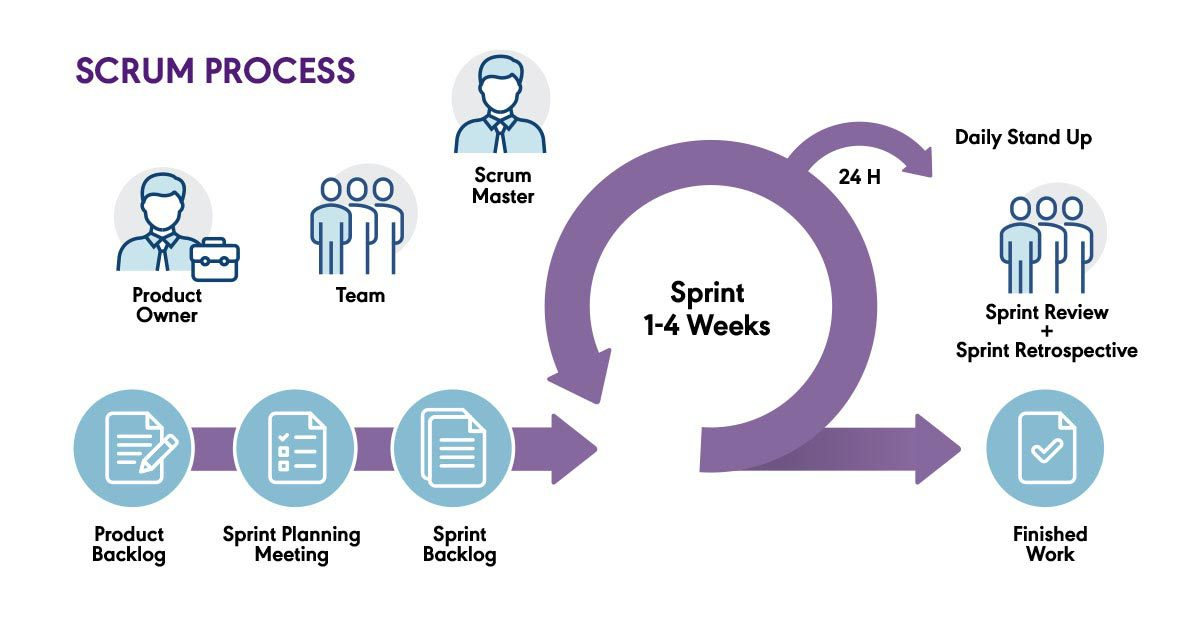
\includegraphics[width=\textwidth]{../Images/scrum.jpg}
    \caption{Approche itérative et incrémentale adoptée (inspirée du cadre Scrum).}
\end{figure}

Comme décrit dans le \textit{Scrum Guide} \cite{scrumguide2020}, cette approche repose sur des itérations courtes, une collaboration étroite avec les utilisateurs et une amélioration continue, Comprendre un peu plus le processus scrum.

\begin{enumerate}
\item \textbf{Trois piliers soutiennent l’implémentation d’un contrôle empirique de processus}

La Transparence, l’Inspection et l’Adaptation.
	\begin{itemize}
	\item \textbf{La transparence :} requiert la définition d’un standard commun pour ces aspects afin que les observateurs partagent une compréhension commune de ce qui est observé.
	\item \textbf{L’inspection :} les utilisateurs de Scrum doivent fréquemment inspecter les artefacts Scrum et l’état d’avancement par rapport à un objectif de Sprint (Sprint Goal) afin de détecter les écarts indésirables. La fréquence de ces inspections ne devrait pas gêner le travail en cours. Ces inspections sont bénéfiques lorsqu’elles sont effectuées de manière diligente sur les lieux du travail par les personnes qualifiées.
	\item \textbf{L’adaptation :} si un inspecteur détermine qu’un ou plusieurs aspects du processus dérivent hors des limites acceptables, et que le produit qui en résulte sera inacceptable, le processus ou le matériel utilisé par le processus doit être ajusté. Un ajustement doit être fait dès que possible afin de minimiser le risque d’autres dérives.
	\end{itemize}
	
\item \textbf{Les rôles de scrum}

	Scrum définit un modèle d’équipe optimisant la flexibilité, la créativité et la productivité.
	\begin{itemize}
	\item \textbf{Le Product Owner :} Est un membre à part entière de l’équipe Scrum représentant des clients et utilisateurs dans le cadre du projet. Il est en charge de la tenue du backlog produit.
	\item \textbf{Développement team :} Est constituée de professionnels qui produisent à chaque Sprint un incrément « terminé » et potentiellement livrable du produit. Ils ont toutes les compétences nécessaires pour effectuer le travail sans dépendre de personnes n’appartenant pas à l’équipe. Transforme un besoin exprimer par le Product Owner en fonctionnalités utilisable. L’équipe est responsable de livrer à la fin de chaque sprint les items qui ont été priorisés pour ce sprint.
	
	\item \textbf{Scrum Master:} Est une personne qui maîtrise le Scrum et qui s’assure que ce dernier est correctement appliqué. Il a un rôle de coach à la fois auprès du Product Owner et auprès de l’équipe de développement
	\end{itemize}

\item \textbf{Les événements du Scrum}

Les événements prescrits par Scrum créent de la régularité et minimisent la nécessité d’autres réunions non prévues. Tous les événements sont limités dans le temps, de telle sorte que chaque événement ait une durée maximale. 

\begin{itemize}
\item \textbf{Sprint :} est une période (constante) d’un mois au maximum, au bout de laquelle l’équipe livre un incrément du produit, potentiellement livrable. Chaque Sprint doit avoir un objectif qui est un but fixé et peut être réalisé par l’implémentation d’une partie du Product Backlog

\item \textbf{Sprint planning :} Le travail à effectuer dans le Sprint est prévu dans la réunion de planification de Sprint. Elle est d'une durée maximale de quatre heures pour les sprints de deux semaines L'équipe Scrum discute des fonctionnalités qui peuvent être développées pendant le Sprint. Le Product Owner fournit des clarifications sur les articles du Backlog du produit. L'équipe sélectionne les éléments du Backlog de produit pour le Sprint, car ils sont les meilleurs pour évaluer ce qu'ils peuvent accomplir dans le Sprint.

\item \textbf{Le Daily Meeting :} Est une réunion de 15 minutes pour l'équipe, menée quotidiennement pour comprendre rapidement le travail depuis la dernière réunion quotidienne de Scrum. Cette réunion est également appelée réunion quotidienne debout. Pendant la réunion, chaque membre de l'équipe explique :

\begin{itemize}
\item Qu'a-t-il fait hier pour aider l'équipe à atteindre l'objectif de sprint?
\item Que va-t-il faire aujourd'hui pour aider l'équipe à atteindre le but du sprint?
\item Voit-il des obstacles qui l'empêchent, lui ou l'équipe, de rencontrer le but du sprint?
\end{itemize}
\item \textbf{Sprint review:} À la fin de chaque sprint, l'équipe scrum et le client se réunissent pour effectuer la revue de sprint, sa durée maximale est de quatre heures pour un sprint de 4 semaines. L'objectif de la revue de sprint est de valider l'incrément de produit qui a été réalisé pendant le sprint.

\item \textbf{Sprint Rétrospective :} Est une réunion faite par l’équipe Scrum. Elle a pour but l'adaptation aux changements qui surviennent au cours du projet et l'amélioration continue du processus de réalisation
\end{itemize}

\item \textbf{Les artefacts du Scrum }

Les artefacts de Scrum sont spécialement conçus pour maximiser la transparence d’informations essentielles afin que tous en aient la même compréhension. Les artefacts de Scrum sont :
\begin{itemize}


\item \textbf{Product Backlog :} Est une liste ordonnée de tous les éléments identifiés comme nécessaires au produit. Il constitue l’unique source d'exigences pour tout changement à apporter au produit. Le Product Owner est responsable du Product Backlog, y compris son contenu, sa disponibilité et son ordonnancement. Le Product Backlog évolue au fur et à mesure que le produit et le contexte dans lequel il sera utilisé évoluent. Il est dynamique ; il change constamment pour identifier ce que le produit requiert pour être approprié, compétitif et utile.

\item \textbf{Sprint Backlog :} Est l’ensemble des éléments sélectionnés pour le Sprint plus un plan pour livrer l’incrément du produit et réaliser l’objectif du Sprint. Le Sprint Backlog est une prévision que l’équipe de développement fait de la fonctionnalité qui sera présente dans le prochain incrément et le travail nécessaire pour livrer cette fonctionnalité dans un incrément « Fini ».

\item \textbf{L'incrément :} Est constitué des éléments du Backlog produit « Finis » pendant le sprint ainsi que de la valeur cumulative des incréments livrés dans les sprints précédents. À la fin d’un Sprint, le nouvel incrément doit être « Fini », ce qui implique qu’il doit être dans un état publiable
\end{itemize}
\end{enumerate}


Cette démarche a permis de livrer des premières versions utilisables dès les premières semaines de développement, de recueillir des retours fréquents, et d’ajuster les fonctionnalités au plus proche du besoin métier.

\subsubsection{Cadrage progressif et centrage utilisateur}

Dès les premières phases du projet, une approche résolument \textbf{centrée sur l'utilisateur} a été adoptée afin de garantir l'adéquation entre les solutions développées et les besoins concrets du terrain. Plutôt que de suivre un cahier des charges figé, l’équipe projet a misé sur un processus itératif fondé sur l'observation, l’échange, et l’expérimentation.

Cette démarche s’est articulée autour de plusieurs leviers complémentaires :

\begin{itemize}
    \item \textbf{Entretiens exploratoires} : En amont du développement, des échanges approfondis ont été menés avec les techniciens de maintenance, les chefs d’atelier ainsi que les utilisateurs finaux. Ces entretiens visaient à identifier les usages existants, les frustrations liées aux outils précédents, et les attentes implicites souvent non formulées dans les documents formels. Cette phase a permis de dresser une cartographie fine des besoins fonctionnels et ergonomiques.

    \item \textbf{Prototypage et tests en conditions réelles} : Chaque livraison intermédiaire a été conçue comme un prototype fonctionnel, testé directement dans les ateliers dans une base de données test. Ces tests ont permis d’évaluer la pertinence des choix de conception face à la réalité du terrain, de détecter des points de friction, et d’itérer rapidement. Ce processus a contribué à affiner progressivement l’interface, les flux de navigation, et les messages contextuels.
 
    \item \textbf{Démonstrations régulières et feedbacks itératifs} : Des sessions de démonstration ont été organisées à chaque étape clé du développement. La présence active de la tutrice en entreprise et des référents métier a permis de recueillir des retours immédiats, concrets et contextualisés. Ces échanges ont joué un rôle essentiel dans l’ajustement rapide des fonctionnalités, en maintenant un alignement constant avec les objectifs opérationnels.

    \item \textbf{Documentation intégrée et évolutive} : Un effort particulier a été porté sur la clarté de l’accompagnement utilisateur. Chaque livrable était accompagné de contenus d’aide embarqués : guides de saisie, info-bulles contextuelles, vérifications en temps réel et messages explicites en cas d’erreur. Cette documentation progressive a évolué en parallèle du produit, en fonction des retours utilisateurs et des cas d’usage identifiés.
\end{itemize}

\noindent Cette approche de cadrage progressif, fondée sur la proximité avec les utilisateurs et l’ajustement en continu, a permis de concevoir une solution réellement adaptée au contexte métier, tout en favorisant l’appropriation rapide par les équipes.

\newpage
\subsubsection{Structuration du travail}

Afin d’assurer une progression fluide et maîtrisée du projet, la mission a été découpée en cinq grandes étapes, chacune correspondant à une phase clé du cycle de développement. Cette structuration temporelle et méthodologique a permis de garantir la cohérence globale tout en laissant de la place à l’itération et à l’ajustement.


\paragraph{Temps d'alternance} 

L’organisation du temps sur les deux années d’alternance s’est articulée autour de quatre grands volets : la formation académique, le travail en entreprise, les périodes de stage et les périodes de congés. Cette répartition, illustrée dans le graphique ci-dessus, reflète l’équilibre entre apprentissage théorique, mise en pratique en situation réelle, et temps de repos réglementaire.

\vspace{1em}
\begin{itemize}
    \item \textbf{13,8 mois en entreprise} : Cela représente la majorité du temps d’alternance. Ces mois ont été consacrés à l’accomplissement des missions confiées chez Jeumont Electric, au développement des applications web, à la co-conception avec les équipes métiers et au déploiement progressif des outils sur le terrain. Cette immersion prolongée dans un environnement industriel a permis une montée en compétences rapide, une compréhension fine des besoins métier, et une participation active à la digitalisation des processus critiques.

    \item \textbf{8 mois en formation} : Cette partie a permis d'acquérir les fondements théoriques en informatique, gestion de projet, développement web, cybersécurité, et méthodologies Agiles. Ces acquis ont été directement mis en œuvre dans les projets réalisés en entreprise, favorisant un aller-retour permanent entre théorie et pratique.

    \item \textbf{5 mois en période de stage} : Tout d’abord, j’ai débuté en stage au sein de l’entreprise, avant de poursuivre en alternance sur le site de Carquefou. Cette continuité a permis de livrer des résultats plus aboutis sur le plan technique, en mettant l’accent sur la mise en production, la documentation et les tests utilisateurs. Elle a également été l’occasion de capitaliser sur le travail déjà réalisé, tout en développant une autonomie renforcée dans la conduite du projet.

    \item \textbf{2,2 mois de vacances} : Ces périodes regroupent les congés payés, les jours fériés, les RTT et les éventuels ponts. Bien que non productives au sens strict, elles ont permis de maintenir un équilibre indispensable à la qualité du travail et à l’engagement sur le long terme.
\end{itemize}


\begin{figure}[H]
    \centering
    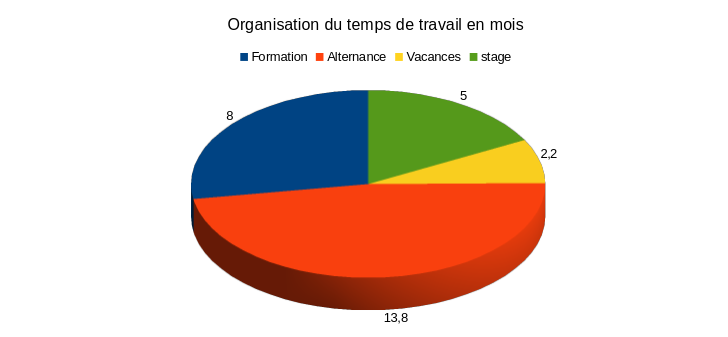
\includegraphics[width=0.8\textwidth]{../Images/organisation.png}
    \caption{Structure - temps d'alternance}
\end{figure} 

Cette répartition du temps a permis de structurer une alternance à la fois exigeante et formatrice, avec un fort ancrage terrain et une continuité pédagogique adaptée au rythme industriel.
\\

\paragraph{Structuration en Entreprise}

\begin{enumerate}
    \item \textbf{Cadrage et recueil des besoins (mois 1–2)}\\
    Cette première phase a consisté à poser les bases du projet. Des observations terrain et des entretiens ciblés ont permis de mieux comprendre les processus existants, les points de difficultés rencontrés par les utilisateurs, ainsi que les attentes fonctionnelles. Ces éléments ont ensuite été formalisés sous forme de cahiers des charges simplifiés et de périmètres applicatifs précis.

    \item \textbf{Conception et modélisation (mois 1-2)}\\
    À partir des besoins identifiés, un travail de conception a été mené pour modéliser les données, structurer les flux et esquisser les interfaces. Cette étape a donné lieu à la production de schémas de base de données relationnelles, de maquettes d’écrans interactifs, et de cartes de flux décrivant les interactions entre les différentes entités métier.

    \item \textbf{Développement  (mois 10)}\\
    La réalisation technique s’est appuyée sur une logique de développement itératif, organisée en lots fonctionnels. Trois applications principales ont été développées, chacune répondant à un besoin métier distinct. Des tests unitaires ont été intégrés dès cette phase pour sécuriser les fonctionnalités clés, et les premiers retours utilisateurs ont permis d’ajuster en continu les développements.

    \item \textbf{Tests utilisateurs et validation (mois 1-2)}\\
    Une série de tests en conditions réelles a été menée auprès d’un panel d’utilisateurs cibles. Ces tests ont permis de valider la conformité des outils aux usages attendus, de corriger certains dysfonctionnements, et de finaliser la documentation associée : guides de prise en main, messages d’aide, procédures spécifiques.

    \item \textbf{Mise en production et accompagnement (mois 1)}\\
    La dernière phase a marqué le déploiement effectif des outils dans l’environnement interne de l’entreprise. Des sessions de formation ont été organisées pour faciliter la montée en compétence des équipes. Un transfert de compétences a également été assuré afin de garantir l’autonomie future de l’entreprise dans la gestion et l’évolution des applications.
    \item \textbf{Documentation technique (mois 2)} 
    
La documentation technique a été un livrable central du projet, élaborée de manière progressive tout au long de la mission. Elle se compose de deux volets complémentaires :

\begin{itemize}
    \item \textbf{Le dossier de programmation} : il contient l’ensemble des informations liées à l’architecture logicielle (MVC Symfony), les schémas de base de données, les choix technologiques, la structure des entités, ainsi que les procédures de déploiement sur serveur Debian. Ce dossier vise à faciliter la reprise du code source par un autre développeur en assurant clarté, maintenabilité et traçabilité du projet.
    
    \item \textbf{Le manuel d’utilisation} : destiné aux utilisateurs finaux (techniciens, chefs de projet, responsables etc ...), ce guide explique comment naviguer dans l’application, créer une fiche, valider une étape, générer un rapport ou consulter l’historique. Il est illustré par des captures d’écran, des parcours utilisateurs types et des réponses aux questions fréquentes (FAQ).
\end{itemize}

Cette documentation permet de transmettre les clés techniques et fonctionnelles nécessaires à la bonne exploitation des outils, et assure leur pérennité dans l’écosystème numérique de l’entreprise.
\end{enumerate}


\subsection{Conclusion}

Ce chapitre a permis de cadrer précisément la mission menée au sein de Jeumont Electric, en identifiant les enjeux techniques, fonctionnels et organisationnels auxquels elle répond. La digitalisation ciblée de processus industriels, initiée par le site de Carquefou, s’est appuyée sur une démarche Agiles, collaborative et orientée utilisateur. Le projet a pu évoluer de manière itérative et pragmatique, tout en gardant le cap sur des objectifs concrets : fiabilité des données, réduction des tâches manuelles, valorisation du savoir-faire et pilotage en temps réel. Cette base méthodologique et organisationnelle constitue le socle sur lequel se sont appuyés les développements présentés dans le chapitre suivant.



\newpage
\section{Conception et développement des applications web}
Ce chapitre revient sur la phase opérationnelle de la mission. Après la phase d’analyse des besoins métiers et d’établissement d’un cadre méthodologique adapté, vint l’étape de conception et développement de trois applications web visant à satisfaire chacun des trois besoins exprimés sur le site de Carquefou. Ces outils ne sont pas de simples prototypes, mais des outils en cours d’utilisation, d’appréciation et d’évolution.


\subsection{Présentation des trois applications}
Au cours de la mission, trois applications web indépendantes mais complémentaires ont été développées. Chacune répond à un besoin métier spécifique, identifié sur le terrain avec les équipes techniques, de production et de maintenance. 

\begin{enumerate}
    \item \textbf{Base d’expertise}
    \\
    Cette application a pour objectif de centraliser, fiabiliser et historiser les expertises techniques (électriques et mécaniques) réalisées sur les machines tournantes. Elle remplace un système basé sur des fichiers Excel, des rapports papier, et des échanges par e-mail, peu adaptés aux exigences de traçabilité et de capitalisation.

Elle permet notamment de :
\begin{itemize}
    \item Centraliser les expertises électriques et mécaniques dans une base unique.
    \item Saisir les relevés de mesures (isolement, faux-ronds, jeux, équilibrage…),
        \item Uniformiser la structure des rapports pour tous les secteurs (nucléaire, industrie…).

    \item Associer des observations et préconisations par étape d’expertise,
    \item Joindre des photos, documents ou contrôles externes,
    \item Générer automatiquement les rapports (expertise et final) normalisé PDF,
    \item Rendu plus robuste et traçable.
\end{itemize}
Grâce à cette application, les techniciens saisissent les données directement après intervention, et les chefs de projet disposent d’un rapport formel en quelques clics. Le gain de temps, la cohérence documentaire et la préservation du savoir-faire sont significatifs.

    \item \textbf{Traçabilité des barres - TraQbar}
    \\
    Cette seconde application concerne la gestion des barres Roebel utilisées dans la fabrication des stators. Chaque barre doit être tracée depuis la découpe du brin du cuivvre jusqu’à sa mise en place dans le stator.
    
L’objectif est de garantir :
\begin{itemize}
    \item une visibilité complète sur chaque étape de fabrication,
    \item l’identification des opérateurs et des dates d’action,
        \item Suivre l'évolution d'une barre à travers les étapes de production : formage, isolation, cuisson, essais ECE, stockage.

    \item la détection rapide de non-conformités ou de retards,
    \item la capacité à reconstituer le parcours exact de chaque barre.
        \item Déclarer et historiser les non-conformités par poste avec motif, photo et traitement appliqué.
            \item Bloquer automatiquement l’avancement d’une barre en cas de défaut ou d'étape non validée.
    \item Suivre l'évolution de la fabrication d'une barre ou des barres
        \item Afficher un tableau de suivi en temps réel pour chaque affaire ou chaque opérateur.
    \item Voir le reporting d'une affaire
    \item Fournir une synthèse consolidée de l'affaire avec export PDF de toutes les étapes et historiques.
        \item Importer ou exporter les données liées aux barres (format CSV ou Excel) pour analyse externe.
    \item Import et export des données de la base
\end{itemize}

L’interface permet de consulter l’état de chaque barre en temps réel, avec une vue globale de la production. Un code barre est généré pour chaque barre, facilitant les intégrations futures avec d’autres systèmes (étiquetage, scan mobile…).  Les audits de Jeumont Electric s'appuient en confiance sur le TraQbar (preuve qualité et robustesse des données

    \item \textbf{Suivi budgétaire maintenance}
    \\
    Enfin, la troisième application a été conçue pour faciliter le pilotage budgétaire des opérations de maintenance (interventions internes ou externes).

Elle répond à un besoin concret des responsables de service : avoir une vision claire des coûts par machine, atelier, période ou type d’intervention. L’application permet de :
\begin{itemize}
    \item Créer des fiches d’intervention liées à un équipement,
    \item Saisir les postes de dépenses (pièces, main d’œuvre, prestataires),
    \item Saisir et suivi des budgets
    \item Saisir et Suivi des dépenses sur budget
    \item Générer des indicateurs budgétaires dynamiques,
    \item Exporter les données sous Excel pour reporting ou analyse croisée.
\end{itemize}

L’interface inclut un tableau de bord avec visualisation graphique, alertes en cas de dépassement budgétaire, et filtres pour les responsables.

\end{enumerate}

\subsection{Outils de gestion de projet utilisés}

Afin d’assurer une coordination efficace du projet, plusieurs outils numériques ont été mobilisés pour répondre aux besoins de planification, de suivi, de documentation et de versionnage. Chacun de ces outils a joué un rôle complémentaire dans l'organisation du travail et la structuration des livrables :

\begin{itemize}
    \item \textbf{GitHub} : plateforme de gestion de version utilisée pour l’hébergement du code, le suivi des modifications via des commits, la gestion des branches de développement, ainsi que la documentation des bugs et des demandes de fonctionnalités via les \textit{issues}. GitHub a permis un développement structuré, itératif et traçable.

\begin{figure}[H]
    \centering
    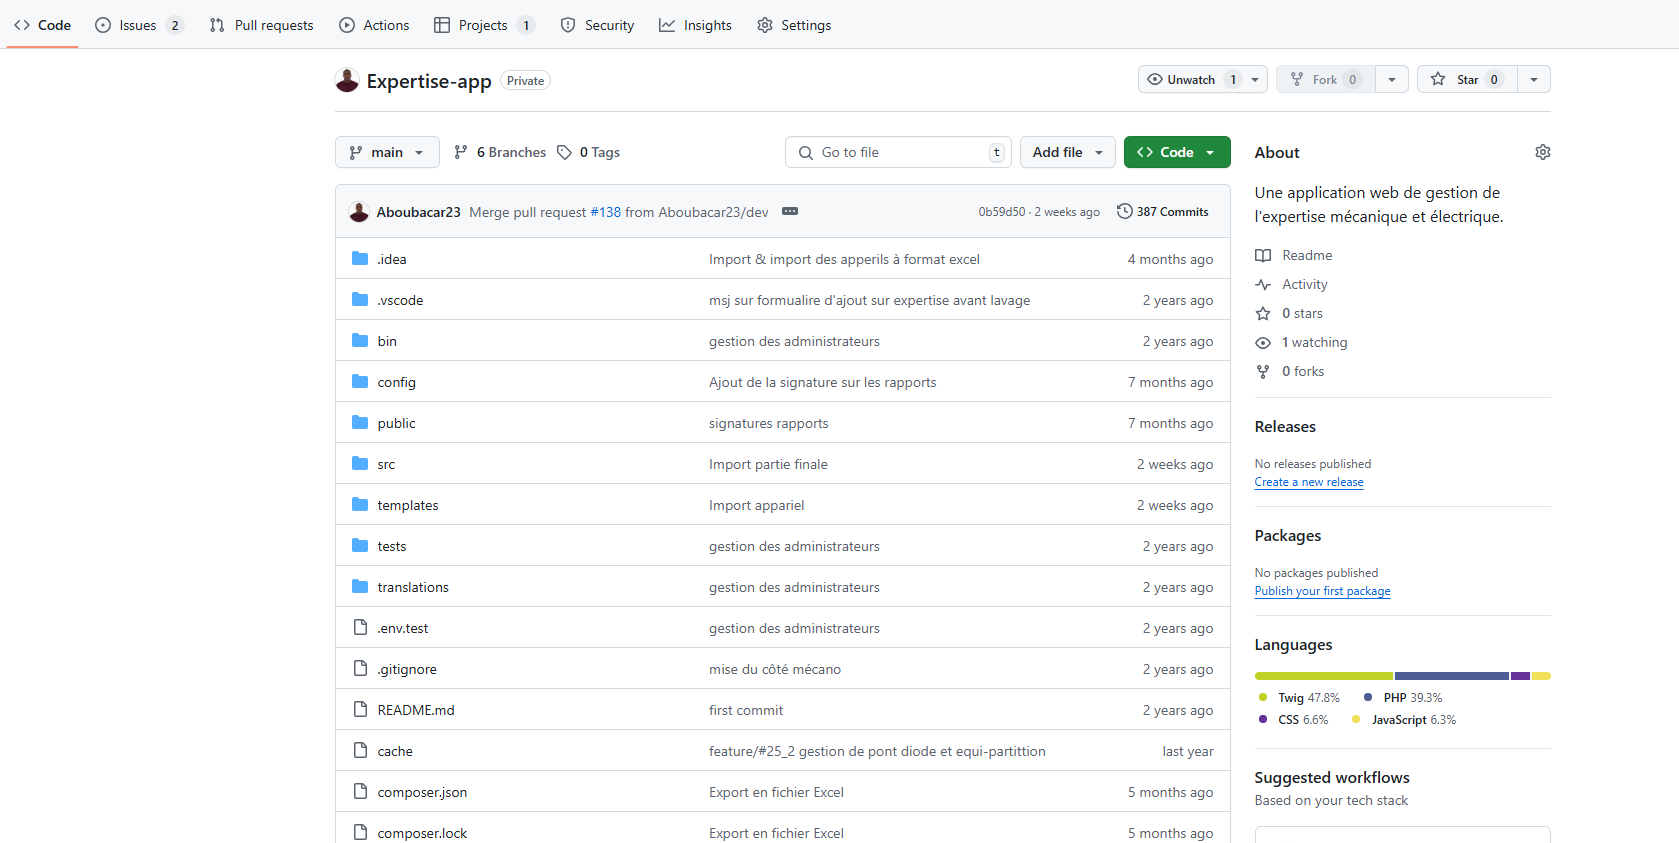
\includegraphics[width=\textwidth]{../Images/github.png}
    \caption{Interface Github.}
\end{figure}

    \item \textbf{Trello} : outil de gestion visuelle des tâches selon une approche kanban. Chaque carte représentait une fonctionnalité, un correctif ou un lot à développer. L’utilisation des colonnes, étiquettes et checklists a facilité le suivi des priorités, des dépendances et de l’avancement de manière collaborative et flexible.
    
\begin{figure}[H]
    \centering
    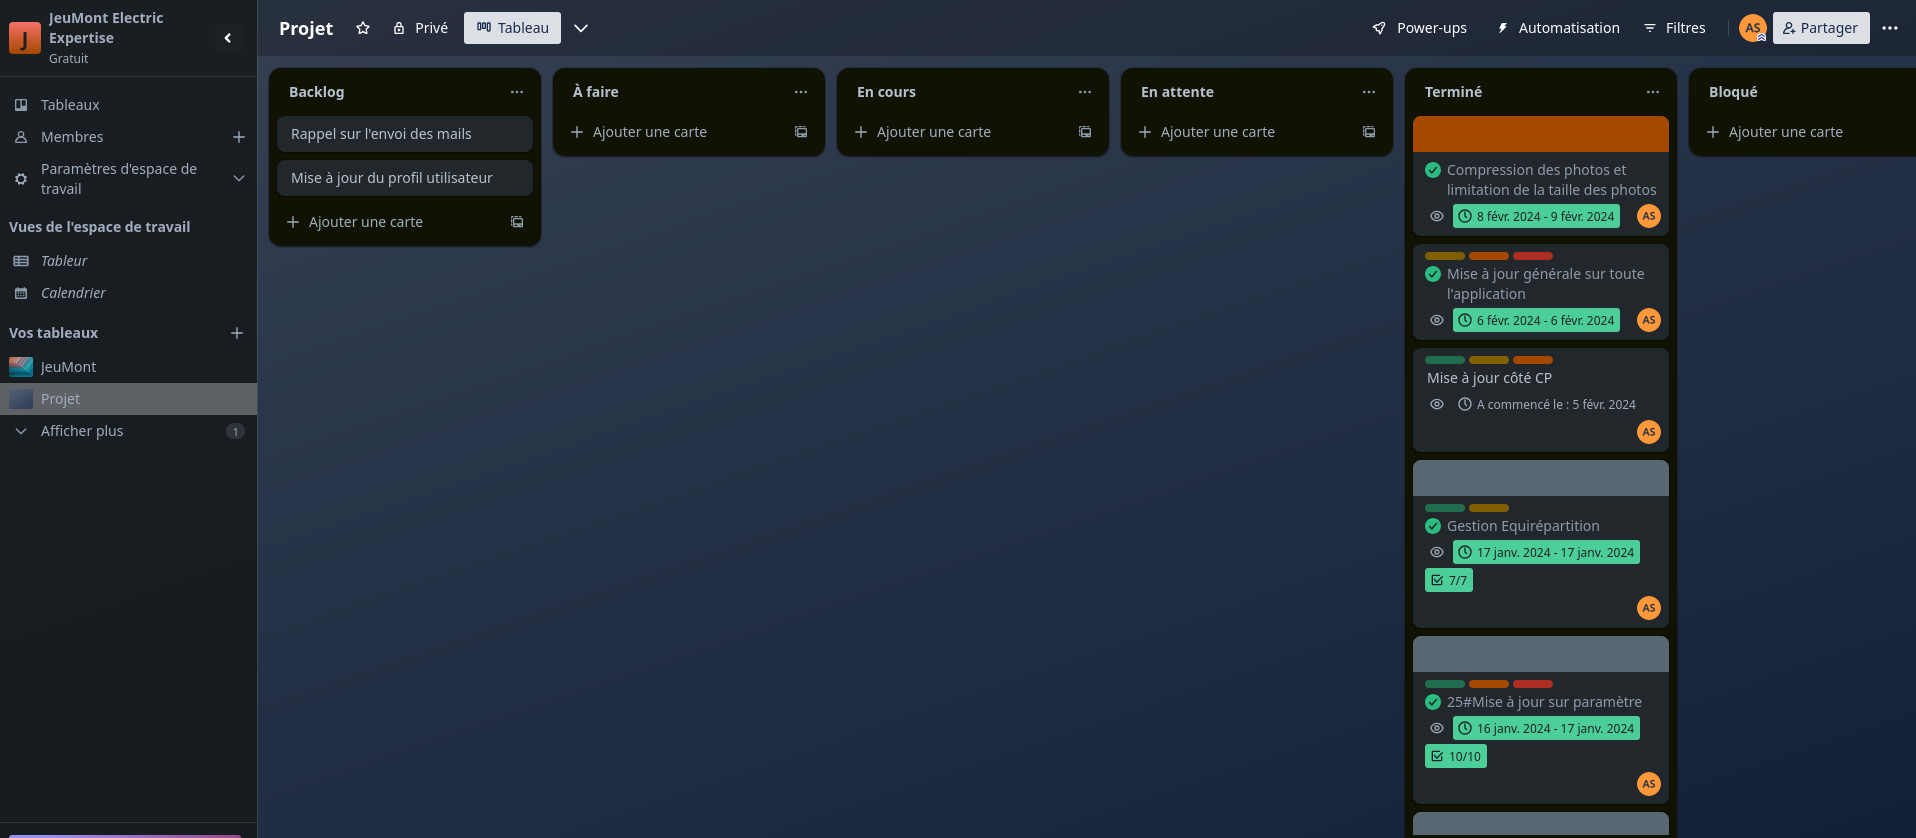
\includegraphics[width=\textwidth]{../Images/trello.png}
    \caption{Extrait trello du projet Base Expertise.}
\end{figure}

   \vspace{0.5em}
    \begin{flushleft}
    \textbf{Légende des couleurs du diagramme :}
	\begin{itemize}[label=--]
    		\item \textbf{Backlog} : tâches recensées mais non encore planifiées.
    		\item \textbf{À faire} : tâches prévues à court terme.
    		\item \textbf{En cours} : tâches en cours de traitement.
    		\item \textbf{En attente} : tâches bloquées ou dépendantes d'autres actions.
    		\item \textbf{Terminé} : tâches finalisées.
    		\item \textbf{Bloqué} : tâches en impasse nécessitant une action extérieure.
	\end{itemize}
    \end{flushleft}


    \item \textbf{GanttProject} : logiciel utilisé pour établir une planification globale du projet à l’échelle macro. Les diagrammes de Gantt ont permis de visualiser la chronologie des phases, les dépendances entre les tâches clés, et les jalons de livraison, tout en assurant une cohérence temporelle avec les objectifs de l’alternance.
    
\begin{figure}[H]
    \centering
    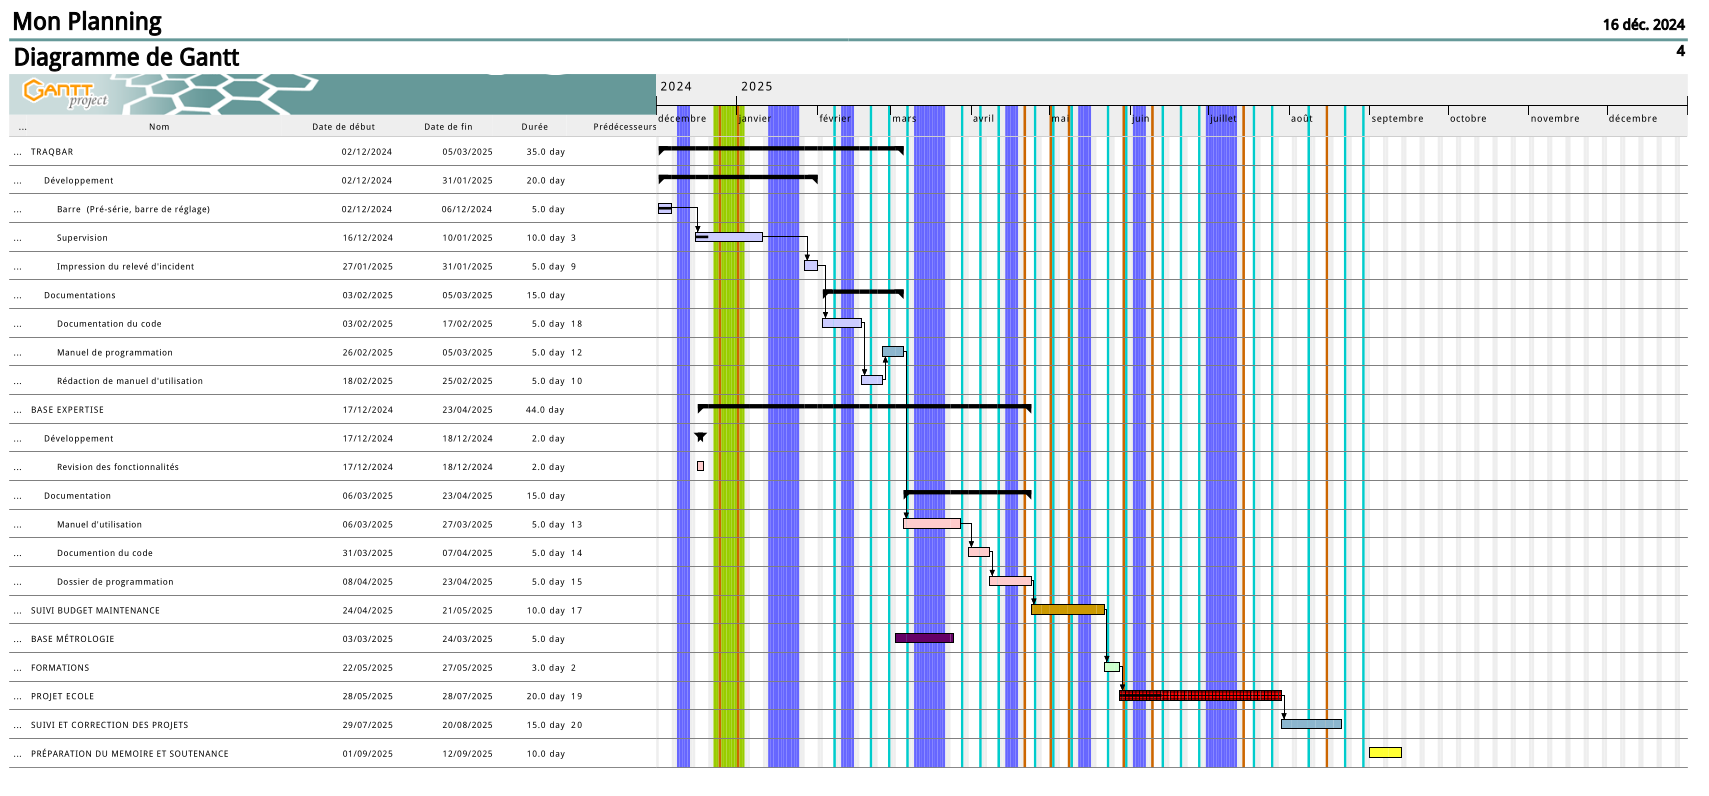
\includegraphics[width=\textwidth]{../Images/planning-2.png}
    \caption{Extrait du planning global de la mission en 2025 réalisé avec GanttProject.}
\end{figure}

   \vspace{0.5em}
    \begin{flushleft}
    \textbf{Légende des couleurs du diagramme :}
    \begin{itemize}
        \item \textcolor[HTML]{C6EFCE}{\textbf{Vert pâle}} : Vacances, Congés
        \item \textcolor[HTML]{FF0000}{\textbf{Rouge}} : Période en entreprise pour la rédaction du mémoire
        \item \textcolor[HTML]{002060}{\textbf{Bleu foncé / Indigo}} : Formation
        \item \textcolor[HTML]{DAE8FC}{\textbf{Bleu clair}} : Jours fériés
    \end{itemize}
    \end{flushleft}
    
    
\begin{figure}[H]
    \centering
    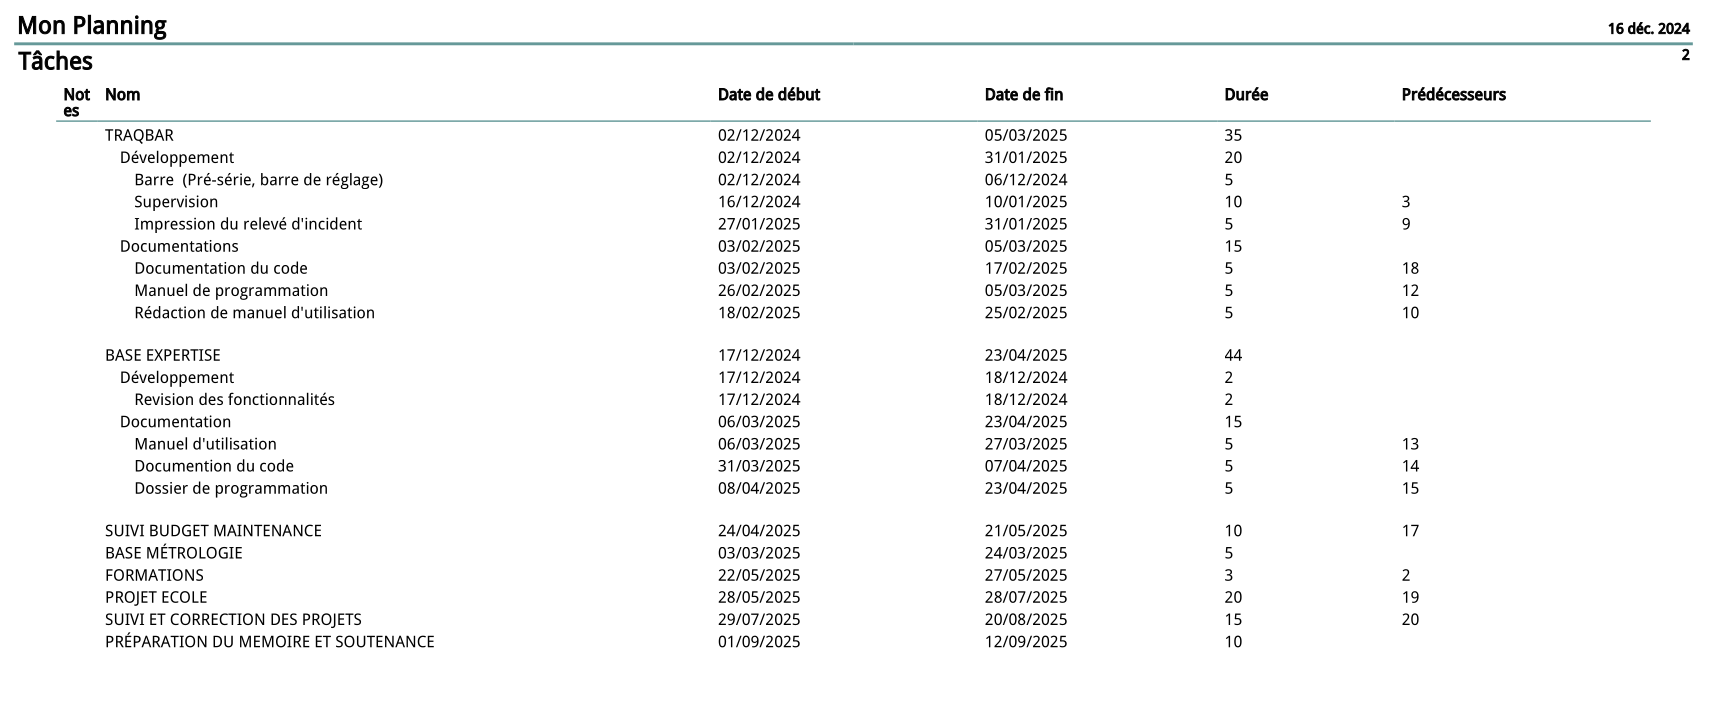
\includegraphics[width=\textwidth]{../Images/planning-sur-2025.png}
    \caption{Extrait du planning en Tâches en 2025.}
\end{figure}	
	
\smallskip
\begin{center}
    \small \textit{Ce diagramme présente les principales phases du projet, avec leurs dates de début et de fin, ainsi que les relations de dépendance entre les différentes tâches. Les couleurs permettent de distinguer les sous-projets ou domaines fonctionnels.}
\end{center}
	
\end{itemize}
	
\subsection{Stack technique}

Pour garantir la robustesse, la maintenabilité et la sécurité des applications développées, un ensemble de technologies éprouvées a été choisi. Le but était d'assurer la compatibilité avec l’infrastructure informatique existante de Jeumont Electric tout en respectant les standards de développement web modernes.

\subsubsection{Technologies utilisées}
Pour mener à bien ces projets, plusieurs technologies ont été mobilisées à chaque étape du développement. Ces outils jouent un rôle fondamental dans la conception, la mise en œuvre, et le déploiement des applications, en assurant robustesse, évolutivité et simplicité d’usage. \\
Voici une présentation synthétique des principales technologies employées tout au long de la mission.
\begin{itemize}

\item \textbf{PHP} : 
est un langage de script côté serveur spécialement conçu pour le développement web. C'est le langage principal utilisé avec le framework Symfony pour mettre en œuvre la logique métier de l'application. Sa syntaxe claire et sa large communauté de développeurs en font l'une des technologies les plus courantes pour créer des applications web dynamiques et interactives.

\item \textbf{Symfony (version 6)} : framework PHP structuré, utilisé pour gérer la logique back-end, les routes, la validation des formulaires, l'accès aux données, la sécurité et l'organisation modulaire du projet.

\item \textbf{Composer } :
Composer est un gestionnaire de dépendances pour PHP. Il facilite l'intégration de bibliothèques tierces dans un projet Symfony. Grâce à Composer, nous pouvons installer et gérer automatiquement les packages dont l'application a besoin, en assurant également leur compatibilité les uns avec les autres. Cela permet d'accélérer le développement et de maintenir l'ensemble du projet à jour avec les dernières versions des dépendances.

\item \textbf{MySQL (v8)} : base de données relationnelle pour la persistance des données. Choisie pour sa compatibilité avec l’existant, sa robustesse et sa capacité à gérer des volumes importants d’informations structurées (expertises, historiques, coûts...).

\item \textbf{Twig} : moteur de templates intégré à Symfony pour générer les vues HTML de manière sécurisée et maintenable.

\item \textbf{JavaScript (vanilla)} : utilisé pour la validation dynamique côté client, les filtres en temps réel et certaines interactions avec l’interface.

\item \textbf{Chart.js} : bibliothèque de visualisation utilisée pour les graphiques de l’application de suivi budgétaire (camemberts, histogrammes, courbes dynamiques).

\item \textbf{PhpSpreadsheet} : outil PHP permettant la génération d’exports Excel (XLSX) depuis l’application.

\item \textbf{DomPDF} : générateur de PDF pour les rapports automatiques d’expertise.

\item \textbf{Serveur web debian : }
le serveur web Debian fait référence à l'utilisation du système d'exploitation Debian pour héberger les applications web. Pour bien finaliser mes missions, j’ai utilisé un serveur Debian pour déploier les travaux réalisés.  Debian est un système d'exploitation Linux réputé pour sa stabilité, sa sécurité et sa facilité de gestion. En utilisant Debian comme serveur web, l'application peut bénéficier d'un environnement fiable et bien maintenu.
\end{itemize}

Toutes les technologies ont été choisies en open-source pour garantir leur pérennité, leur flexibilité d’évolution, et leur facilité de documentation.

\subsubsection{Architecture Globale}

Le bon fonctionnement des applications développées repose sur une architecture technique à la fois robuste, modulaire et adaptée aux exigences du milieu industriel. Afin de garantir une haute disponibilité, une sécurité renforcée et une évolutivité à moyen terme, une approche en deux volets a été adoptée : une architecture logique (organisation interne des composants logiciels selon le modèle MVC) et une architecture physique (infrastructure matérielle et réseau déployée localement sur le site de Carquefou). Cette structuration claire a permis d’assurer la performance, la maintenabilité et l’interopérabilité des outils au sein du système d’information existant de Jeumont Electric.

\paragraph{Architecture logique}
Les applications développées dans le cadre de cette mission reposent sur une architecture web de type client-serveur classique, parfaitement adaptée à l’environnement industriel du site de Carquefou. Cette architecture permet une séparation claire des responsabilités entre les couches logiques du système, facilitant la maintenance, l’évolutivité, et l’intégration future à d’autres outils internes.

Chaque application suit le modèle MVC (Modèle-Vue-Contrôleur), implémenté via le framework Symfony. Cette structure permet une organisation du code claire, une réutilisabilité des composants, et un découplage efficace entre la logique métier, l’interface utilisateur et la persistance des données.
\begin{enumerate}
\item \textbf{Modèle (Model)} : Les entités Doctrine représentent les objets métier (Expertise, Barre, Intervention, Utilisateur, etc.) et assurent l’interface avec la base de données relationnelle MySQL. Les entités sont typées, validées, et liées entre elles via des relations bien définies.
\item \textbf{Vue (View)} : Les vues sont générées dynamiquement avec Twig, le moteur de template de Symfony. Chaque écran est conçu de manière ergonomique, avec une logique d’affichage claire, adaptée aussi bien aux écrans de bureau qu’aux tablettes utilisées sur le terrain.
\item \textbf{Contrôleur (Controller)} : Chaque action utilisateur (consultation, saisie, validation, export) est gérée par un contrôleur Symfony qui orchestre la récupération des données, la logique métier, les règles de sécurité et la génération de la réponse HTTP.

\end{enumerate}

\begin{figure}[H]
    \centering
    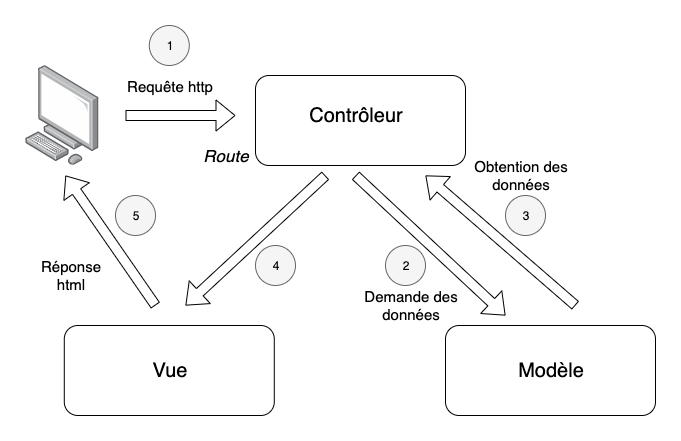
\includegraphics[width=0.9\textwidth]{../Images/architecture-logique.png}
    \caption{Architecture logique – modèle MVC}
    \label{fig:architecture_logiciel}
\end{figure}

Cette organisation a permis de mutualiser les bonnes pratiques de développement sur l’ensemble des modules applicatifs, tout en garantissant une homogénéité de structure et de fonctionnement. L’architecture est restée volontairement modulaire pour autoriser, à terme, une réutilisation des composants (formulaires, contrôleurs, styles).

Il faut tout d'abord retenir que le contrôleur est le chef d'orchestre : c'est lui qui reçoit la requête du visiteur et qui contacte d'autres fichiers (le modèle et la vue) pour échanger des informations avec eux.

Le fichier du contrôleur demande les données au modèle sans se soucier de la façon dont celui-ci va les récupérer. Par exemple : «Affiche moi la liste des affaires. Le modèle traduit cette demande en une requête grâce à L'ORM, récupère les informations et les renvoie au contrôleur.
Une fois les données récupérées, le contrôleur les transmet à la vue qui se chargera d'afficher la liste des demandes. Le rôle de contrôleur ne se limite pas à faire la jonction entre le modèle et la vue mais il se charge aussi à faire d'autres opérations par exemple des calculs, des vérifications
d'autorisations ou miniaturiser des images, etc.
Concrètement, le visiteur demandera la page au contrôleur et c'est la vue qui lui sera retourné. Bien entendu, tout cela est transparent pour lui, il ne voit pas tout ce qui se passe sur le serveur. C'est sur ce type d'architecture que repose un très grand nombre de sites professionnels.

\paragraph{Architecture physique} 

Les applications réalisées dans le cadre de cette mission sont hébergées localement sur l’infrastructure informatique de Jeumont Electric, selon une architecture de type client-serveur. Ce choix repose sur des critères à la fois techniques et organisationnels : maîtrise des données, sécurité du réseau, évolutivité des modules, et facilité d’accès depuis différents postes utilisateurs (bureau, atelier, logistique).

Cette architecture garantit une séparation claire entre les postes clients (utilisateurs finaux), le serveur applicatif (logique métier) et le serveur de base de données (stockage structuré). Elle respecte également les bonnes pratiques de déploiement d’applications web internes dans un environnement industriel.


\begin{enumerate}
\item \textbf{Client : }
Les utilisateurs accèdent aux applications via un navigateur web standard (Google Chrome ou Firefox), installé sur :
	\begin{itemize}
    \item des ordinateurs fixes de bureau (chefs de projet, ingénieurs) ;
    \item des PC industriels placés en atelier (techniciens) ;
    \item ou des tablettes mobiles connectées au réseau Wi-Fi sécurisé du site.
	\end{itemize}

Aucun logiciel n’est à installer côté client : l’interface utilisateur est entièrement générée côté serveur puis rendue dynamiquement dans le navigateur. Cette architecture permet une maintenance simplifiée et une grande flexibilité dans l’usage, tout en évitant les problèmes liés aux versions locales ou à la compatibilité logicielle.

\item \textbf{Serveur :}
Le serveur hébergeant les applications est une machine Linux (Debian), configurée avec :
\begin{itemize}
    \item le serveur HTTP (Apache 2 ou Nginx) pour la réception des requêtes,
    \item le framework Symfony pour gérer la logique applicative,
    \item et les services système nécessaires (cron jobs, pare-feu, logs).
\end{itemize}

Ce serveur est sécurisé par mot de passe, accessible uniquement au personnel habilité (administrateurs systèmes), et régulièrement sauvegardé. Le code source est versionné via Git, et les déploiements sont effectués manuellement ou via des scripts de mise à jour.


\item \textbf{ Base de données - MySQL}

L’ensemble des données critiques (utilisateurs, expertises, barres, dépenses, historiques...) est stocké dans une base de données MySQL, hébergée sur la même machine ou sur un serveur dédié selon les besoins. La base suit un modèle relationnel structuré autour d’identifiants uniques, de clés étrangères et de contraintes d’intégrité.

Elle est sauvegardée quotidiennement, avec un archivage hebdomadaire sur une machine distante. Les accès sont restreints au seul serveur applicatif, interdisant toute connexion directe depuis les postes clients.

\item \textbf{ Sécurité et confidentialité}

Le système d’authentification repose sur les composants de sécurité Symfony. L’accès aux applications nécessite une authentification avec identifiant et mot de passe. Selon le rôle attribué à l’utilisateur (technicien, responsable, administrateur), certaines sections sont restreintes (validation, export, suppression...).

Toutes les requêtes critiques sont protégées contre les attaques classiques (CSRF, injection SQL) via les mécanismes de protection intégrés de Symfony.


\end{enumerate}

\vspace{1em}

\begin{figure}[H]
    \centering
    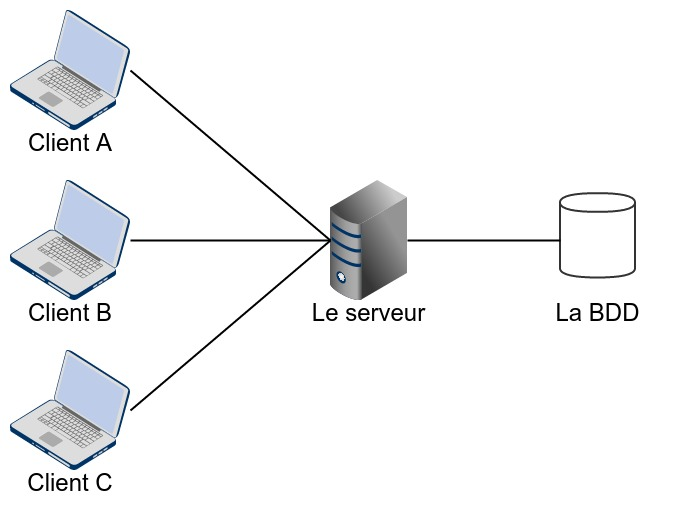
\includegraphics[scale=0.45]{../Images/ClientServeur.jpeg} % Mets ici le vrai chemin vers l'image renommée
    \caption{Architecture physique – Architecture client-serveur}
    \label{fig:architecture_physique}
\end{figure}

Cette architecture permet aujourd’hui à l’ensemble des services concernés de disposer d’outils numériques fiables, accessibles, et sécurisés, tout en restant compatibles avec les contraintes techniques du site industriel de Carquefou.

\paragraph{Schéma d’architecture générale}

Le schéma ci-dessous présente l’organisation fonctionnelle globale des applications développées dans le cadre de cette mission. Il illustre les composants principaux, leurs interactions, ainsi que la circulation des données entre le client, le serveur et la base de données.

\begin{figure}[H]
    \centering
    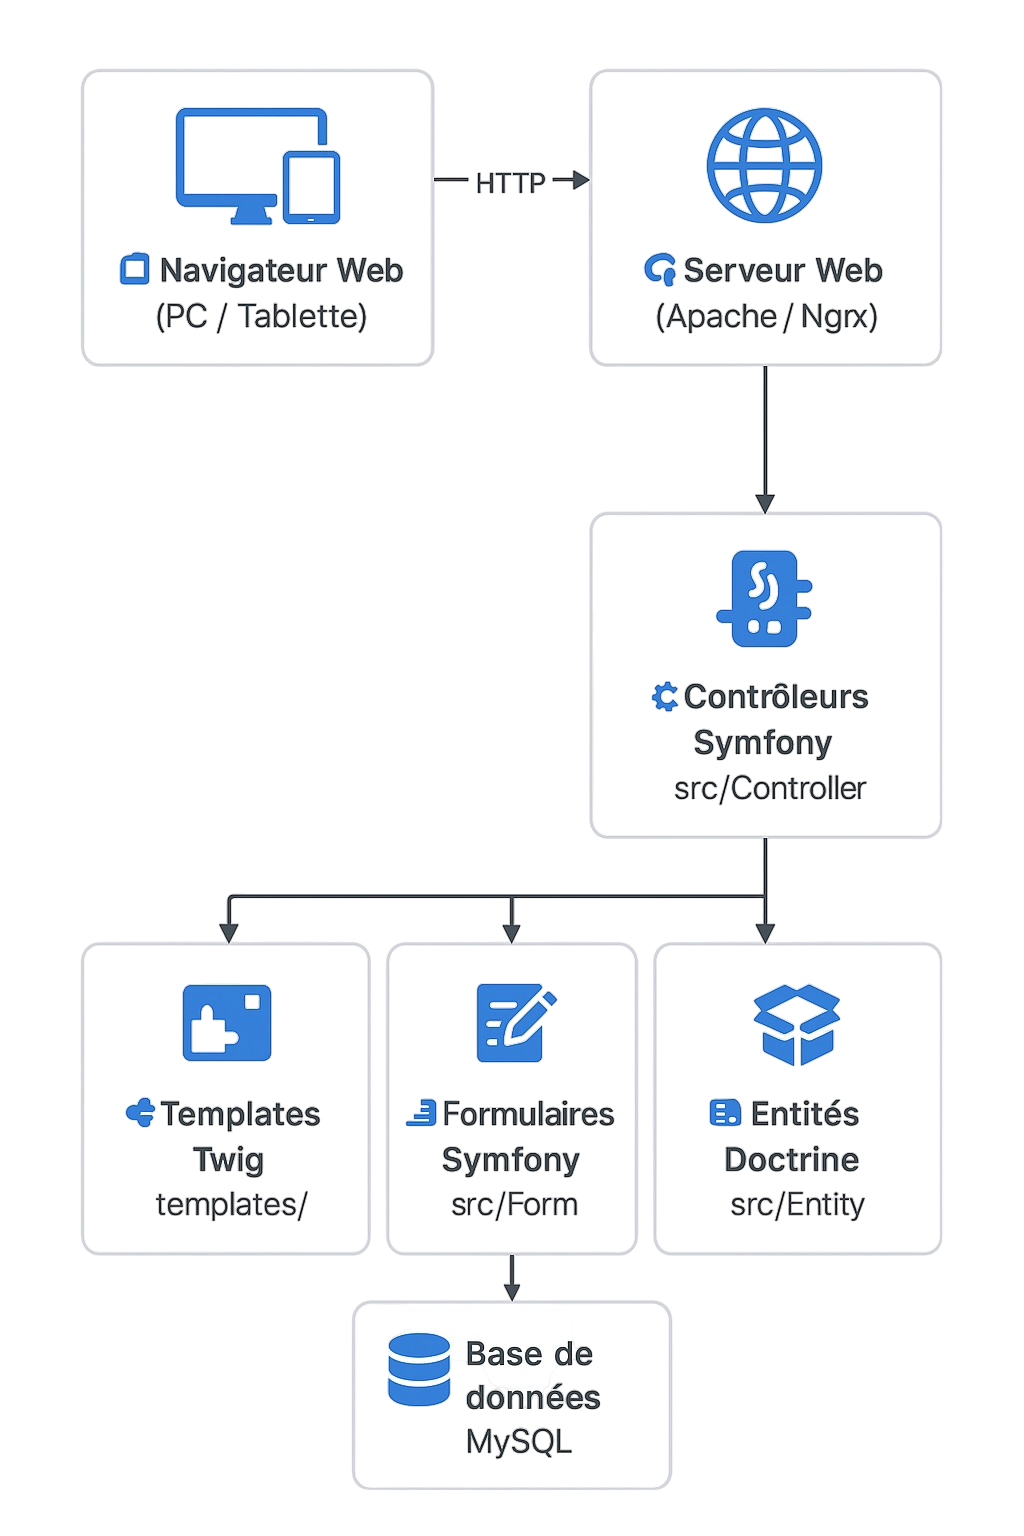
\includegraphics[scale=0.30]{../Images/schema_composant} % adapter le nom du fichier
    \caption{Schéma de composants – Architecture fonctionnelle des applications}
    \label{fig:schema_composants}
\end{figure}

L’architecture repose sur une logique modulaire, où chaque couche est responsable d’un rôle bien distinct : présentation, logique métier, persistance des données. Cela permet une grande lisibilité du code, une répartition des responsabilités, et une facilité de maintenance ou d’ajout de nouvelles fonctionnalités à l’avenir.

\paragraph*{Légende du schéma de composants}

\begin{table}[H]
\centering
\begin{tabular}{|p{4.5cm}|p{10cm}|}
\hline
\textbf{Composant} & \textbf{Rôle dans l’architecture} \\
\hline
\textbf{Navigateur Web (Client)} & Interface utilisateur : permet l’interaction avec les applications (saisie, consultation, validation). Accessible sur PC ou tablette. \\
\hline
\textbf{Serveur Web (Apache ou Nginx)} & Réceptionne les requêtes HTTP du navigateur et les redirige vers les contrôleurs Symfony. Gère également les ressources statiques (CSS, JS, images). \\
\hline
\textbf{Contrôleurs Symfony} & Point d’entrée logique des actions utilisateur. Gèrent les appels métier, les vérifications, et les redirections vers les vues. \\
\hline
\textbf{Formulaires Symfony} & Encapsulent la logique de création et de validation des données saisies. Sécurisent les entrées utilisateurs. \\
\hline
\textbf{Templates Twig} & Vues HTML dynamiques générées selon les données reçues. Responsables de l’affichage côté client. \\
\hline
\textbf{Entités Doctrine (Model)} & Représentation des objets métiers (expertises, barres, dépenses, utilisateurs). Liaison avec la base MySQL via ORM. \\
\hline
\textbf{Base de données MySQL} & Stockage centralisé de toutes les données de l’application. Optimisée pour la traçabilité, l’intégrité et la performance. \\
\hline
\end{tabular}
\caption{Légende des composants principaux de l’architecture}
\label{tab:legende_composants}
\end{table}

Cette architecture modulaire, robuste et documentée constitue un socle fiable pour les applications développées. Elle respecte les bonnes pratiques du développement web moderne tout en s’adaptant aux contraintes industrielles du terrain.



\paragraph{Sécurité, accessibilité et interopérabilité}

\begin{itemize}
\item \textbf{ Sécurité :}

\begin{itemize}
    \item \textbf{Authentification basée sur Symfony Security} : contrôle d’accès par rôles (ex. : technicien, superviseur).
    \item \textbf{Vérifications serveur + client} : les formulaires sont protégés contre les injections, les valeurs sont validées côté serveur et côté client.
    \item \textbf{CSRF tokens activés} : pour prévenir toute tentative d’interaction malveillante avec les formulaires.
    \item \textbf{Log des actions critiques} : insertion, modification, validation, suppression.
\end{itemize}

\item \textbf{ Accessibilité :}

Les applications ont été conçues pour être lisibles, rapides et accessibles à tout collaborateur, même non expert. Les polices, tailles, contrastes et boutons suivent les recommandations WCAG pour une expérience utilisateur inclusive.

\item \textbf{ Interopérabilité :}

Bien que les outils soient autonomes, leur conception respecte les bonnes pratiques pour un éventuel futur interfaçage :

\begin{itemize}
    \item Structuration claire de la base de données avec des identifiants communs.
    \item Export de données dans des formats standards (CSV, XLSX, PDF).
    \item Possibilité d’intégrer des API REST à l’avenir pour échanger avec d’autres systèmes (ERP, GMAO).
\end{itemize}

Cette architecture assure un excellent équilibre entre simplicité, performance et évolutivité. Elle permet aujourd’hui d’adresser les besoins exprimés, tout en ouvrant la voie à une montée en puissance progressive des outils numériques de l’entreprise.

\end{itemize}

\subsection{Réalisation des projets}
Cette section retrace la phase de réalisation concrète de la mission. Après avoir identifié les besoins métiers et posé un cadre méthodologique rigoureux, l'étape suivante a été de concevoir et développer les applications web. Ces outils ne sont pas de simples prototypes : ils sont aujourd'hui utilisés, appréciés, et amenés à évoluer dans le futur.

\subsubsection{Organisation du projet}

Le projet est structuré selon les principes de la méthode Agile \textbf{Scrum}, permet une organisation flexible, itérative et centrée utilisateur. Ce choix méthodologique a permis d’assurer une réactivité maximale face aux besoins changeants des utilisateurs tout en maintenant un cadre structurant pour le suivi des développements.
\begin{enumerate}

\item \textbf{Rôles clés du projet}
\begin{itemize}
    \item \textbf{Product Owner (PO)} : assuré par les responsables métier (maintenance, technique, production), jouant le rôle de référents pour la définition des besoins et la validation des livrables.
    \item \textbf{Scrum Master / Développeur} : rôle assumé par l’alternant, en charge de l’analyse des besoins, du développement technique, des tests et du suivi de l'avancement.
    \item \textbf{Utilisateurs finaux} : techniciens, chefs de projets, responsables de service, régulièrement impliqués dans les phases de test, démonstration et ajustement.
    
\end{itemize}

\item \textbf{Backlog Product}

Dès les premières phases de cadrage, un \textbf{backlog produit} a été constitué (dans l'annexe). Il regroupait l’ensemble des fonctionnalités attendues, sous forme de \textbf{user stories}, classées par priorité métier. Chaque élément du backlog était rédigé de manière concise (ex. : “En tant que technicien, je veux saisir les mesures d’isolement pour générer un rapport conforme”) et comprenait des critères d’acceptation clairs.

Le backlog évoluait en permanence :
\begin{itemize}
    \item Alimentation régulière via les ateliers utilisateurs et les retours terrain ;
    \item Repriorisation à chaque sprint selon la valeur ajoutée, la complexité et l’urgence métier ;
    \item après chaque livraison de sprint réajouter les tâches n'ont terminé, d’améliorations ou de nouvelles demandes identifiées en cours de projet.
\end{itemize}

\item \textbf{Planification du projet} 

Suite à la définition du \textit{Product Backlog}, nous avons structuré la planification des \textbf{sprints} en respectant une logique de complexité fonctionnelle croissante. Chaque sprint avait une durée fixe de 2 à 4 semaines et ciblait un périmètre applicatif bien défini, avec des livrables concrets attendus à la fin de chaque cycle.

\textbf{Remarque :} Les durées indiquées pour chaque sprint correspondent uniquement aux phases de développement. Les temps consacrés à l’analyse préalable, à la conception fonctionnelle, ainsi qu’aux phases de test et de validation ne sont pas inclus dans ce tableau.

	\begin{enumerate}
	\item \textbf{Planifcation du projet Base d'expertise}
	
\begin{table}[H]
\centering
\begin{tabular}{|c|p{8cm}|c|}
\hline
\textbf{Itération} & \textbf{Titre} & \textbf{Semaines} \\
\hline
Sprint 1 & Mise en place et gestion d'administration & 3 \\
\hline
Sprint 2 & Gestion du module d'expertise technique - ECE & 3 \\
\hline
Sprint 3  & Gestion du module d'expertise technique - Mécanique  & 3 \\
\hline
Sprint 4 & Génération et gestion des rapports d'expertise & 3 \\
\hline
Sprint 5 & Gestion du module Métrologie & 2 \\
\hline
\end{tabular}
\caption{Planification des sprints du projet Base d'expertise}
\label{tab:planification_projet1}
\end{table}

... comme présenté dans le tableau \footnote{Contrairement à la méthode Scrum qui impose des sprints de durée fixe, ce projet applique une approche Agile adaptée. La durée des sprints varie selon la complexité fonctionnelle, les objectifs et les contraintes de calendrier.}.

\newpage
	\item \textbf{Planifcation du projet TraQbar}
	
\begin{table}[H]
\centering
\begin{tabular}{|c|p{8cm}|c|}
\hline
\textbf{Itération} & \textbf{Titre} & \textbf{Semaines} \\
\hline
Sprint 1 & Gestion Administration & 2 \\
\hline
Sprint 2 & Gestion module Technique & 3 \\
\hline
Sprint 3 & Gestion du module Production & 3 \\
\hline
Sprint 4 & Gestion du module suppervision & 3 \\
\hline
Sprint 5 & Gestion rébut,pré-serie, barre de réglage, configuration  & 2 \\
\hline
\end{tabular}
\caption{Planification des sprints du projet TraqBar}
\label{tab:planification_projet2}
\end{table}


	\item \textbf{Planification du projet Suivi Budget}
	
	
\begin{table}[H]
\centering
\begin{tabular}{|c|p{8cm}|c|}
\hline
\textbf{Itération} & \textbf{Titre} & \textbf{Semaines} \\
\hline
Sprint 1 & Gestion module budget et dépense & 2 \\
\hline
Sprint 2 & Gestion du module investissement et dépense  & 2 \\
\hline
\end{tabular}


\caption{Planification des sprints du projet Suivi Budget}
\label{tab:planification_projet1}
\end{table}

	\end{enumerate}
	
\item \textbf{Organisation en sprints}

Le projet a été découpé en \textbf{sprints de 2 à 4 semaines}, chacun dédié à un lot fonctionnel spécifique (ex. : module expertise, suivi des barres, exports budgétaires). À la fin de chaque sprint, une version opérationnelle était livrée puis testée par les utilisateurs concernés.

Chaque sprint comportait les étapes suivantes :
\begin{itemize}
    \item \textbf{Sprint Planning} : définition des fonctionnalités à développer selon les priorités exprimées par les métiers.
    \item \textbf{Développement et tests} : implémentation incrémentale des modules avec tests manuels intégrés.
    \item \textbf{Sprint Review} : démonstration des nouvelles fonctionnalités auprès des utilisateurs (sur poste ou en atelier).
    \item \textbf{Sprint Retrospective} : retour d’expérience sur le sprint, identification des points à améliorer pour les itérations suivantes.
\end{itemize}

\item \textbf{Outils de pilotage Agile}

L'organisation du travail et le suivi des tâches ont été facilités par :
\begin{itemize}
    \item \textbf{Trello} pour la gestion des backlogs et des tâches en cours ;
    \item \textbf{GitHub} pour le versioning, le suivi des commits et le traitement des bugs via des \textit{issues} ;
    \item \textbf{Diagrammes de Gantt} pour assurer une cohérence globale avec le calendrier de l’alternance et les jalons internes de Jeumont Electric.
\end{itemize}

\item \textbf{Livrables intermédiaires}

Chaque fonctionnalité a été livrée au fil de l’eau, testée en conditions réelles puis validée en collaboration avec les utilisateurs. Cette démarche a permis :
\begin{itemize}
    \item une adaptation continue aux retours terrains ;
    \item une appropriation progressive des outils par les équipes ;
    \item une réduction significative des retouches en fin de projet.
\end{itemize}

L’approche Scrum, bien que simplifiée dans le contexte d’une alternance individuelle, a prouvé son efficacité pour mener à bien un projet transversal, avec plusieurs parties prenantes, des contraintes techniques fortes et des délais stricts.
\end{enumerate}


\subsubsection{Parcours utilisateur}

Pour assurer l’adoption rapide et efficace des applications, une attention particulière a été portée à la définition de parcours utilisateur clairs, logiques et adaptés aux usages métiers. Chaque application a été conçue selon une logique de navigation intuitive, afin de permettre aux utilisateurs — qu’ils soient techniciens, superviseurs ou responsables — de réaliser leurs tâches avec un minimum de clics, de ressaisies et de formation.

\paragraph*{Base d’expertise} \

Le parcours utilisateur type commence par la création d’une fiche d’expertise dès la réception d’un équipement. L’utilisateur peut ensuite, selon son rôle :
\begin{enumerate}
    \item Renseigner les mesures mécaniques et électriques étape par étape.
    \item Ajouter des commentaires, constats visuels et préconisations.
    \item Joindre des photos ou documents à chaque étape.
    \item Visualiser une synthèse globale.
    \item Générer automatiquement le rapport d’expertise.
\end{enumerate}
Chaque utilisateur accède uniquement aux étapes pour lesquelles il est habilité (saisie, validation, consultation), assurant à la fois sécurité et fluidité du processus.

\paragraph*{TraQbar (traçabilité des barres)} \

L’interface utilisateur s’articule autour d’une vue par projet ou par affaire. Le technicien sélectionne une barre via un filtre ou un QR code, puis peut :
\begin{enumerate}
    \item Visualiser son historique complet.
    \item Déclarer l’état de la barre à un poste donné.
    \item Signaler une non-conformité, avec  commentaire.
    \item Accéder aux consignes, schémas ou documents associés.
    \item Transmettre automatiquement l’information au poste suivant.
\end{enumerate}
Le responsable de production accède à des vues globales : état des stocks, suivi d’affaire, tableaux de conformité, export Excel.

\paragraph*{Suivi budgétaire maintenance} \

Le chef de service accède à une interface de type tableau de bord :
\begin{enumerate}
    \item Il crée son budget.
    \item Il saisit les dépenses sur un budget : pièces, MO, prestataires.
    \item Il visualise immédiatement l’évolution du budget.
    \item Il génère un rapport ou exporte les données pour analyse.
\end{enumerate}

La logique d’interface est homogène entre les trois outils (menus latéraux, filtres par date ou projet, onglets clairs), ce qui permet à l’utilisateur de retrouver ses repères rapidement et de naviguer sans assistance technique particulière.

\subsubsection{Contraintes et adaptations techniques}

Tout au long du développement des applications, plusieurs contraintes, techniques, organisationnelles ou sécuritaires, ont nécessité des arbitrages, des ajustements, voire des innovations.
\begin{enumerate}


\item \textbf{Contraintes d’infrastructure} 

Le projet devait impérativement être compatible avec l’environnement technique de Jeumont Electric :
\begin{itemize}
    \item Accès via des navigateurs en version contrôlée (pas de dépendance à des modules externes).
    \item Pas d’installation de client lourd (100\% web).
    \item Déploiement sur un serveur interne Debian sécurisé.
\end{itemize}
Ces éléments ont exclu l’usage de frameworks trop modernes ou d’outils nécessitant des ressources serveur importantes (Node.js, Docker, etc.).

\item \textbf{Contraintes de sécurité informatique} \

L’ensemble du code a été conçu selon les bonnes pratiques de Symfony :
\begin{itemize}
    \item Authentification multi-rôles avec restriction d’accès par profil.
    \item Protection CSRF sur les formulaires.
    \item Validation serveur et client (JavaScript) pour éviter les injections.
    \item Journalisation des actions sensibles (suppression, modification).
\end{itemize}

\item \textbf{Contraintes ergonomiques}

Les techniciens utilisent parfois l’outil en atelier, sur des PC industriels ou tablettes :
\begin{itemize}
    \item Interface sobre, peu de couleurs vives (confort visuel).
    \item Éléments larges, clics accessibles avec gants ou stylets.
    \item Limitation des champs de saisie au strict nécessaire.
\end{itemize}

\item \textbf{Contraintes d’organisation projet}


Le développement a été mené en parallèle d’activités de production. Il fallait donc :
\begin{itemize}
    \item Livrer progressivement par lots fonctionnels (agilité, feedback).
    \item Prioriser les modules selon leur impact opérationnel.
    \item Gérer les retours utilisateurs sans interrompre l’activité.
\end{itemize}

\item \textbf{Adaptations spécifiques mises en œuvre} 


Pour répondre à ces contraintes, plusieurs adaptations ont été déployées :
\begin{itemize}
    \item Utilisation d’un système de cache pour limiter la charge serveur.
    \item Gestion des fichiers (photos, rapports) sur un répertoire du projet plutôt qu’en base.
    \item Intégration de composants réutilisables pour les formulaires et tableaux (gain de temps, homogénéité).
    \item Ajout d’un système de versionnement interne pour les rapports générés (traçabilité).
\end{itemize}
\end{enumerate}
Ces adaptations ont permis de livrer des outils robustes, compatibles avec les réalités du terrain et acceptés sans réserve par les équipes métiers.


\subsection{Tests, validations}

La phase de test est une étape primordiale dans le développement d’un projet informatique. Elle sert à garantir le bon fonctionnement du système en détectant et en corrigeant les anomalies et les failles.

\subsubsection{Stratégie de test}

L’ensemble des fonctionnalités développées a fait l’objet de tests manuels systématiques, intégrés en continu au cycle de développement. Cette stratégie, bien que non automatisée, a permis une vérification fine des comportements fonctionnels dans un contexte d’usage réel.

Les tests ont porté sur plusieurs axes :

\begin{itemize}

\item \textbf{Test d'acceptation du cahier des charges :} lors de ce test nous avons vérifié que le cahier des charges reflète correctement les besoins et les fonctionnalités attendues. En plus je me suis assuré que les objectifs de mes missions et les fonctionnalités essentielles sont clairement définis et compris. Beaucoup plus encore nous avons remarqué, que nous avons même dépassé les fonctionnalités définies dans le cahier des charges grâce à la  méthodologie choisie qui est Agile. À la fin de cette etapes les responsables étaient satisfaits et ont validé le document.

\item \textbf{Test d'utilisabilité : }
Ce test a été un grand plus pour aboutir à un résultat final du projet. Nous avons effectué des sessions de tests avec les utilisateurs finaux (techniciens d'atelier, chef projets, agents de maîtrise, vérificateurs, lecteurs, magasiniers) pour évaluer l'ergonomie et l'accessibilité de l'application, en organisant plusieurs réunions avec les utilisateurs. Collecter des retours d'utilisateurs pour identifier les points d'amélioration mais aussi nous assurer que les connexions simultanées des utilisateurs ne causeront pas problème.

 \item \textbf{Tests de validation des formulaires : }  vérification des règles de saisie, gestion des champs obligatoires, affichage de messages d’erreur explicites, gestion des formats (dates, numériques, listes déroulantes).
    
 \item \textbf{Tests fonctionnels} : simulation de parcours utilisateur complets incluant la création, la modification, la suppression, et la validation d’enregistrements, afin d’éprouver les flux applicatifs dans leur logique métier.
    
    \item \textbf{Tests de performance basique} : insertion en masse de données (entre 50 et 100 enregistrements) pour observer les temps de réponse, les comportements de pagination, et la fluidité de navigation dans les interfaces.
    
    \item \textbf{Tests de résilience} : simulation de scénarios dégradés (coupure réseau, saisies invalides, session expirée) pour s’assurer de la robustesse du front-end et de la gestion des erreurs côté serveur.
\end{itemize}

 Pour mieux comprendre les tests et s'assurer qu'ils ont été bien appliqués, nous avons exposé dans le tableau suivant quelques cas de scénarios de tests fonctionnels.
 
 \begin{table}[H]
\centering
\renewcommand{\arraystretch}{1.4}
\begin{tabular}{|p{4cm}|p{4.5cm}|p{5.5cm}|p{2cm}|}
\hline
\textbf{Cas d’utilisation} & \textbf{Demande} & \textbf{Comportement attendu} & \textbf{Résultat} \\
\hline
Test d’authentification & Saisir le login et mot de passe du compte d’administration & Affichage de la page d’administration & Conforme \\
\hline
Test d’ajout d’un admin & Cliquer sur le bouton « Ajouter admin », remplir les champs du formulaire & Ajouter un nouvel admin, afficher un message de confirmation, puis rafraîchir la liste des admins & Conforme \\
\hline
Test de modification d’un admin & Cliquer sur le bouton « Modifier admin », modifier les données du formulaire & Modifier un admin existant et afficher un message de confirmation & Conforme \\
\hline
Test de suppression d’un admin & Cliquer sur le bouton « Supprimer », confirmer la suppression & Supprimer un admin et afficher un message de confirmation & Conforme \\
\hline
Test Changer le mot de passe d'un admin & Cliquer sur l'icon \textbf{password}, renseigner le nouveau mot de passe & Changer le mot de passe d'un admin, puis afficher la liste des admins & Conforme \\
\hline
Test Chercher une affaire existante & Cliquer sur le bouton "affaire existante", renseigner le numéro d'affaire et cliquer le bouton chercher & Afficher les détails et la page d'opération de l'affaire & Conforme \\
\hline
\end{tabular}
\caption{Scénarios de tests fonctionnels}
\end{table}

\subsubsection{Recette utilisateur}

Des sessions de démonstration ont été organisées tout au long du projet, en conditions proches de la réalité d’exploitation. Ces ateliers de recette ont systématiquement associé les utilisateurs finaux à un référent métier (souvent un chef d’atelier ou un responsable de service), afin de recueillir des retours concrets, contextualisés, et immédiatement exploitables.

Les itérations issues de ces retours ont permis d’améliorer significativement l’ergonomie et la pertinence des modules. Parmi les ajustements notables :

\begin{itemize}
    \item Intégration d’un champ « \textit{notes libres} » dans le module d’expertise, permettant de documenter des cas particuliers ou des commentaires informels souvent absents des grilles standardisées.
    
    \item Révision du contraste colorimétrique dans l’application de traçabilité, en particulier pour les statuts de barres non conformes, afin d’assurer une lisibilité optimale en environnement lumineux (atelier, écran industriel).
    
    \item Ajout d’une fonctionnalité d’export Excel, par projet dans le module budgétaire, facilitant les analyses croisées et l’exploitation des historiques hors ligne.
\end{itemize}

\subsection{Conclusion}

Les trois applications développées dans cette mission ont répondu à des besoins concrets identifiés sur le terrain. Grâce à une approche agile, une architecture robuste et une implication continue des utilisateurs, elles ont permis de digitaliser efficacement des processus critiques. Au-delà du développement technique, le projet a renforcé l’autonomie des équipes, fiabilisé les données et amélioré la traçabilité. Ces outils opérationnels posent les bases d’une digitalisation progressive, adaptable à d’autres services ou sites.


\newpage
\section{Bilan critique et perspectives}

Ce chapitre vise une réflexion à l’échelle de la mission en croisant les retours utilisateurs (étude qualitative) et les données objectives (étude quantitative). Il met en lumière les résultats fournis et les limites affichées par la mission et propose des perspectives de développement. L’objectif : valider l’impact avéré des solutions déployées tout en identifié les leviers d’une amélioration continue.Ce bilan inclut également les compétences développées tout au long de la mission et les recommandations pour assurer la pérennité et la réplicabilité du projet.

\subsection{Analyse critique et retour d’expérience}

Cette section présente une évaluation globale du projet, fondée sur les retours utilisateurs et des indicateurs mesurables. Elle permet de dégager les forces, les limites et les enseignements de la solution développée.


\subsubsection{Analyse qualitative}

L’analyse qualitative repose principalement sur les retours exprimés par les utilisateurs finaux des applications : techniciens d’atelier, chefs de projet, responsables maintenance et membres du service technique. Ces retours ont été recueillis de manière informelle tout au long de la mission (démonstrations, tests, observations, échanges directs) ainsi qu’à travers des échanges post-déploiement.

\begin{enumerate}
\item \textbf{Perception globale des utilisateurs :}

De façon générale, l’accueil des applications développées a été très positif au sein des équipes concernées. Les utilisateurs ont exprimé assez rapidement un sentiment de confort accru, de temps gagné et de professionnalisation de leur façon de travailler. La transition vers des outils numériques pensée à leur besoin a été vécue comme un véritable bénéfice au quotidien opérationnel. Plusieurs techniciens notent la facilité d’utilisation, la clarté des interfaces, la fluidité de navigation. 

Le fait que ces outils aient été réalisés de manière collaborative, ayant largement intégré les retours du terrain à chaque phase du projet a permis de renforcer le sentiment d’implication et l’appropriation des outils. Cette mobilisation cohérente a favorisé une adoption rapide et fluide, sans rejet, ni résistance au changement et a accru la confiance des utilisateurs dans leur adéquation.

\item \textbf{Points forts relevés par les utilisateurs :}

Les premiers retours recueillis sur le terrain mettent en évidence plusieurs atouts majeurs des applications développées. Ces points positifs ont été régulièrement mentionnés au fil des tests, des démonstrations et des phases d’utilisation réelle, et illustrent la manière dont ces outils ont su répondre aux attentes concrètes des utilisateurs finaux. Une synthèse des bénéfices les plus fréquemment relevés :

\begin{itemize}
    \item \textbf{Ergonomie claire et accessible} : avec une interface épurée, des formulaires intuitifs et une structure logique des pages, la prise en main a été rapide, même pour les utilisateurs peu aguerris à l’outil numérique.
    
    \item \textbf{Centralisation de l’information} : la suppression des fichiers dispersés et des versions multiples a amélioré la cohérence des données, tout en facilitant leur consultation en temps réel par les différents services.
    
    \item \textbf{Standardisation des documents} : les rapports générés automatiquement sont désormais uniformisés, mieux structurés et plus facilement exploitables, ce qui renforce leur qualité perçue en interne comme auprès des clients.
    
    \item \textbf{Réduction du stress administratif} : en supprimant les tâches répétitives liées à la saisie manuelle ou à la recherche documentaire, les applications ont contribué à alléger la charge mentale des opérateurs et à fluidifier les flux de travail.
\end{itemize}

\item \textbf{Suggestions et attentes exprimées :}

Malgré ces retours globalement positifs, les utilisateurs ont également formulé des suggestions d’amélioration, preuve de leur engagement :

Ce besoin légitime d’appropriation par les utilisateurs s’est notamment traduit par une série de propositions d’amélioration particulièrement concrètes. Recueillies lors des échanges informels d’une part, et d’autre part dans le cadre des retours de déploiement, ces suggestions marquent le souhait qu’un mieux soit fait, s’avérant donc très utiles pour envisager les prochaines versions : 

	\begin{itemize}
    		\item Ajout d’une option d’import au format Excel en base d’expertise, permettant de renseigner pour chaque barre une date de début et d'une date de fin par poste, mais aussi au statut de la barre à chaque étape du processus.
    		\item Mise en place d'un système de filtres multiples efficaces pour mieux filtrer les recherches dans ce module.
     
\end{itemize}
\end{enumerate}


\subsubsection{Analyse quantitative}
En complément des retours qualitatifs fournis par les utilisateurs, plusieurs indicateurs quantifiables ont été signalés afin d’évaluer l’impact direct des applications sur le fonctionnement de l’entreprise. Certaines données sont en construction, mais les premiers chiffres observés sont déjà évocateurs

\begin{enumerate}

\item \textbf{Réduction du temps de production documentaire}

Avant la mise en place de l’application Base d’expertise, la rédaction d’un rapport prenait en moyenne entre 1h30 et 2h par affaire, en raison des ressaisies, de la mise en forme manuelle et de la recherche de documents. Avec la génération automatique intégrée, ce temps est désormais estimé entre 3 à 5 secondes selon les cas.

\begin{itemize}
    \item \textbf{Temps moyen de rédaction d’un rapport} :
    \begin{itemize}
        \item Avant : \textbf{1h45}
        \item Après : \textbf{3 s}, en un click
        \item \textbf{Gain estimé} : ~99,95\% de temps économisé par rapport.
    \end{itemize}
\end{itemize}

\item \textbf{Fiabilité et exhaustivité des données saisies}

Grâce aux formulaires contrôlés (champs obligatoires, plages numériques valides, listes déroulantes), on observe une baisse sensible des oublis ou incohérences dans les rapports.

\begin{itemize}
    \item \textbf{Nombre moyen d’erreurs de saisie constatées par mois} :
    \begin{itemize}
        \item Avant : ~10–15
        \item Après : 0–2
    \end{itemize}
\end{itemize}

\item \textbf{Traçabilité des interventions}

Sur l’application TraQbar, chaque barre est désormais historisée automatiquement, ce qui permet de reconstituer son parcours complet à tout moment. Avant la mise en place de l’outil, ces données étaient fragmentées, parfois perdues ou difficiles à croiser.

\begin{itemize}
    \item \textbf{Nombre moyen de barres traçables à 100\% (avant vs après)} :
    \begin{itemize}
        \item Avant : \textasciitilde 60–70\% (données parfois incomplètes ou manuelles)
        \item Après : \textbf{100\%}
    \end{itemize}
\end{itemize}

\item \textbf{Adoption par les utilisateurs}

Dès les premières semaines de déploiement, les utilisateurs se sont approprié les outils avec peu de formation nécessaire. La simplicité de l’interface et la proximité avec les besoins exprimés ont facilité cette adoption.

\begin{itemize}
    \item \textbf{Utilisateurs actifs après 1 mois} : 100\% des techniciens concernés sur les 3 postes pilotes.
    \item \textbf{Taux de satisfaction estimé} : supérieur à 90\% d’après les retours exprimés oralement ou lors des tests de validation.
\end{itemize}

\item \textbf{Synthèse}

Ces premiers résultats mettent en évidence des gains concrets sur :
\begin{itemize}
    \item La productivité documentaire,
    \item La fiabilité et la structuration des données,
    \item L’autonomie des utilisateurs,
    \item La traçabilité des opérations critiques.
\end{itemize}

Ces données chiffrées permettent de valider la pertinence de la solution mise en œuvre et de renforcer les arguments en faveur d’un déploiement à plus grande échelle.
\end{enumerate}

\begin{figure}[H]
    \centering
    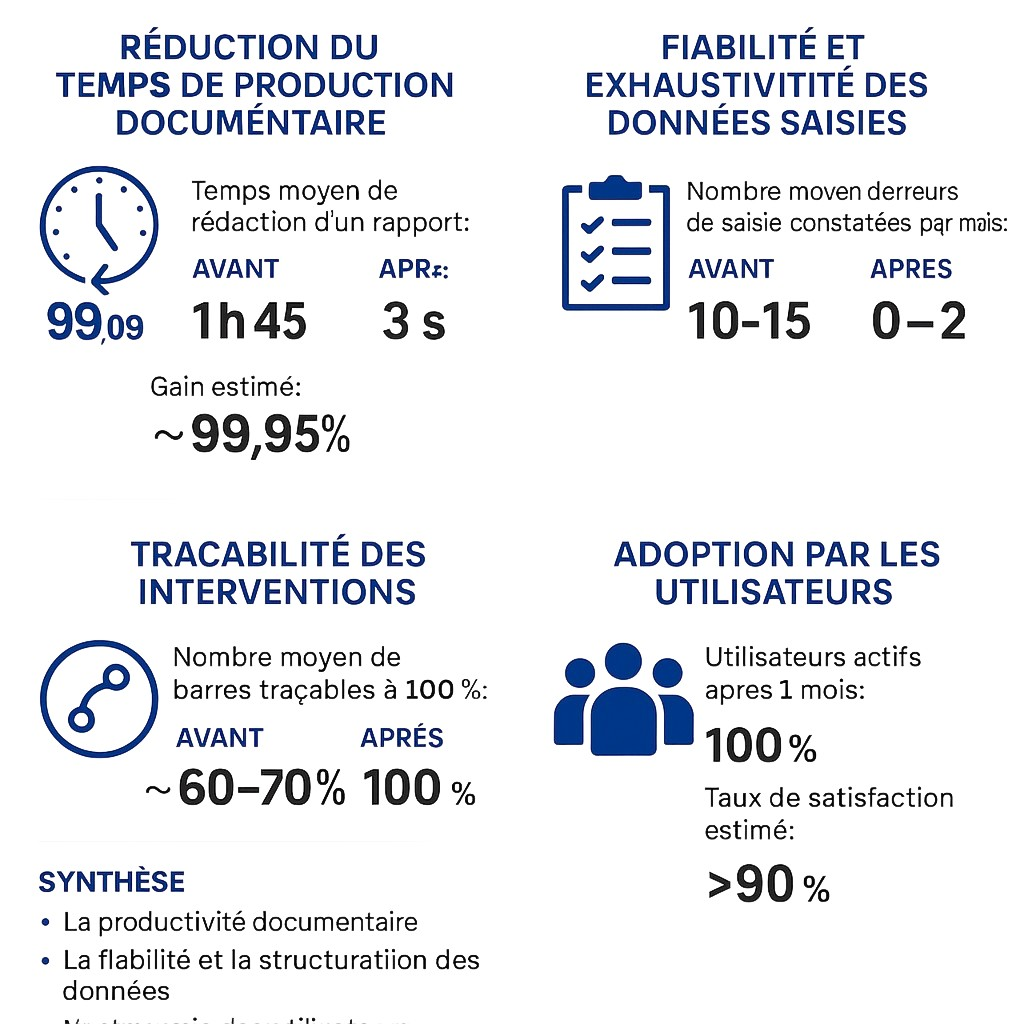
\includegraphics[width=0.9\textwidth]{../Images/bilan_quantitative.jpg}
    \caption{Bilan quantitative}
    \label{fig:architecture_logiciel}
\end{figure}


\newpage
\subsubsection{Résultats globaux}

Au terme de la mission, les applications mises en places ont permis d’engendrer des résultats concrets, tangibles, tant au niveau opérationnel, organisationnel que stratégique. Les retours des utilisateurs, comme les premières observations sur le terrain, témoignent de la pertinence de cette transformation numérique ciblée.

\paragraph{Gains pour l’entreprise :}

\begin{itemize}
    \item \textbf{Fiabilisation des données critiques} : la saisie encadrée et validée par étape limite les erreurs et garantit une meilleure qualité de l’information remontée.

    \item \textbf{Réduction du temps de traitement} : les utilisateurs ont constaté une baisse significative du temps passé à la rédaction des rapports d’expertise, à la recherche documentaire ou à la compilation des données budgétaires.

    \item \textbf{Amélioration de la traçabilité} : chaque action est désormais historisée et associée à un utilisateur, une date, un poste. Les non-conformités peuvent être analysées plus facilement, ce qui alimente la démarche qualité.

    \item \textbf{Standardisation des rapports et documents} : les rapports d’expertise sont harmonisés sur l’ensemble des affaires, conformes aux exigences internes et facilement exportables en PDF.

    \item \textbf{Pilotage en temps réel} : les chefs de projet et responsables sont en mesure d’accéder à des tableaux de bord dynamiques, de suivre des états d’avancement ou de visualiser des indicateurs pertinents.

    \item \textbf{Renforcement de l’image professionnelle} : la présentation claire, structurée et digitalisée des livrables valorise le savoir-faire de Jeumont Electric auprès de ses clients.
\end{itemize}

\paragraph{Améliorations concrètes observées :}

\begin{itemize}
    \item \textbf{Réduction des erreurs de saisie} grâce aux champs contrôlés, aux menus déroulants et à la logique métier intégrée (plages de tolérance, blocs obligatoires).
    
    \item \textbf{Réactivité accrue} en cas de non-conformité : les notifications internes permettent d’agir rapidement, sans attendre une validation manuelle en fin de ligne.
    
    \item \textbf{Meilleure collaboration interservices} : les différentes équipes accèdent aux mêmes données centralisées, ce qui fluidifie la communication et évite les doublons ou pertes d’information.
    
    \item \textbf{Historique facilement exploitable} : possibilité de retrouver une expertise, une barre ou un budget sur des affaires antérieures en quelques clics, sans dépendance aux classeurs Excel éparpillés.
\end{itemize}

\newpage
\subsubsection{Analyse SWOT des projets réalisés}

Afin de compléter l’analyse des résultats, une lecture stratégique a été conduite sous forme de matrice SWOT (Forces, Faiblesses, Opportunités, Menaces). Elle permet d’évaluer la portée des applications développées pour Jeumont Electric, au regard de leur impact à court, moyen et long terme.

\begin{table}[H]
\centering
\renewcommand{\arraystretch}{1.4}
\begin{tabular}{|p{7cm}|p{7cm}|}
\hline
\multicolumn{2}{|c|}{\textbf{Analyse SWOT}} \\
\hline
\textbf{Forces (Strengths)} &
\textbf{Faiblesses (Weaknesses)} \\
\hline
\begin{itemize}[leftmargin=*]
    \item Solutions adaptées aux besoins réels du terrain
    \item Rapidité de développement et de mise en œuvre
    \item Forte adhésion des utilisateurs
    \item Traçabilité renforcée des opérations critiques
    \item Automatisation de tâches à faible valeur ajoutée
\end{itemize}
&
\begin{itemize}[leftmargin=*]
    \item Dépendance aux ressources internes pour la maintenance
    \item Absence actuelle de test automatisé ou CI/CD
    \item les applications ne sont pas automatiquement adapter aux autres sites de l'entreprise.
\end{itemize}
\\
\hline
\textbf{Opportunités (Opportunities)} &
\textbf{Menaces (Threats)} \\
\hline
\begin{itemize}[leftmargin=*]
    \item Réplicabilité sur d’autres sites ou services
    \item Intégration possible avec d’autres outils métiers (ERP, GMAO)
    \item Amélioration continue par itérations fonctionnelles
    \item Renforcement de la stratégie digitale du Groupe
\end{itemize}
&
\begin{itemize}[leftmargin=*]
    \item Risque de non-suivi post-alternance
    \item Changement d’organisation ou de priorités internes
    \item Perte de savoir-faire si non transféré en interne
    \item Qualité des données entrées, notamment rigueur pour les barres
\end{itemize}
\\
\hline
\end{tabular}
\caption{Matrice SWOT}
\label{tab:swot}
\end{table}

Cette lecture synthétique permet de positionner les résultats de la mission dans une perspective stratégique, en identifiant les leviers à exploiter, les limites à adresser, et les conditions de réussite à long terme.

\subsubsection{Montée en compétences}

Cette mission en alternance n’a pas seulement eu pour but de mettre en application des connaissances théoriques acquises en formation, mais a surtout eu valeur de prise de conscience d’un développement personnel et professionnel au sein d’un environnement industriel exigeant face aux enjeux concrets aux impacts opérationnels.

\paragraph{Compétences techniques développées :}

\begin{itemize}
    \item \textbf{Bonne maîtrise du framework Symfony} : compréhension du modèle MVC, gestion des routes, formulaires, sécurité, migration de base, optimisations.
    
    \item \textbf{Bonne onception de bases de données relationnelles} : modélisation des entités métier, relations Doctrine, structuration des schémas MySQL adaptés à des volumes évolutifs.

    \item \textbf{Déploiement en environnement Linux} : configuration de serveurs Apache/Nginx, gestion des permissions, scripts de mise en production.

    \item \textbf{Travail avec des outils professionnels} : GitHub (versionnage, branches), Trello (gestion Agile), GanttProject (planification), Excel avancé (tests, validations).

    \item \textbf{Développement web orienté utilisateur} : amélioration de l’ergonomie, réflexion sur l’accessibilité, création d’interfaces épurées et robustes avec Twig, Bootstrap, Tailwind.
\end{itemize}

\paragraph{Compétences humaines et transversales :}

\begin{itemize}
    \item \textbf{Analyse des besoins métier} : écoute active des utilisateurs, reformulation fonctionnelle, confrontation des exigences aux contraintes techniques.

    \item \textbf{Adaptabilité} : capacité à ajuster les priorités, réagir aux imprévus, intégrer des changements de dernière minute ou des retours terrain.

    \item \textbf{Gestion de projet} : planification, suivi, coordination avec les parties prenantes, arbitrages entre charge de travail et délais.

    \item \textbf{Communication technique} : vulgarisation des choix techniques, création de supports clairs (documentation utilisateur, guides de prise en main).

    \item \textbf{Autonomie et rigueur} : organisation personnelle, respect des jalons, attention portée à la qualité du code et à la maintenabilité.
\end{itemize}

Cette expérience m’a permis de comprendre que le rôle de développeur ne se limite pas à écrire du code, mais qu’il consiste aussi à concevoir des solutions utiles, utilisables et utilisées, en lien direct avec les attentes du terrain. Elle a renforcé ma capacité à raisonner comme un professionnel capable de dialoguer aussi bien avec les métiers qu’avec les équipes techniques.


\subsection{Perspectives et recommandations}

Les applications développées dans le cadre de cette mission ontété développées afin de répondre aux attentes en terme de réponse à des problématiques de terrain. Leur mise en oeuvre alimentera en revanche les nombreuses évolutions techniques, organisationnelles et stratégiques possibles. Cette section propose des pistes d’amélioration ainsi que des recommandations pour assurer la pérennité et la réplicabilité des solutions mises en oeuvre. 

\subsubsection{Évolutions techniques possibles}

Plusieurs fonctionnalités complémentaires pourraient être envisagées à court ou moyen terme :

\begin{itemize}
    \item \textbf{Importer les graphique en pdf}, pour facilté la visualisation des graphes en pdf .
    \item \textbf{Support multi-langue} pour préparer l’outil à une utilisation internationale ou multisite.
    \item \textbf{Connexion plus avancées} , ajouter une fonctionnalité qui permettra aux utilisateurs de se connecter via le badge employé.
\item 
\end{itemize}

\subsubsection{Recommandations pour l’organisation}

Sur le plan organisationnel, certaines conditions sont essentielles pour assurer la réussite à long terme du projet :

\begin{itemize}
    \item \textbf{Désigner un référent applicatif par service}, chargé de centraliser les retours, proposer les évolutions, et former les nouveaux utilisateurs.
    \item \textbf{Planifier des revues semestrielles} avec les utilisateurs pour collecter les retours et hiérarchiser les demandes d’amélioration.
    \item \textbf{Inclure l’application dans les rituels qualité et production} (ex. : bilan mensuel, points projet, suivi maintenance).
    \item \textbf{Capitaliser les bonnes pratiques} issues de cette expérience (documents de formation, vidéos internes, fiches erreurs fréquentes).
\end{itemize}

\subsubsection{Réutilisabilité dans d’autres sites ou services}

L’approche modulaire adoptée dans ces développements permet d’envisager leur extension ou duplication :

\begin{itemize}
    \item Les applications peuvent être déployées sur d’autres sites de Jeumont Electric, moyennant un paramétrage adapté (profils utilisateurs, référentiels internes, contraintes réseau).
    \item Certains modules (comme la photothèque, les tableaux de bord ou la gestion des rapports) peuvent être réutilisés dans d’autres projets internes, voire intégrés dans des outils existants.
    \item La méthodologie employée (approche Agile, co-conception, prototypage rapide) peut servir de modèle pour d’autres initiatives numériques au sein de l’entreprise.
\end{itemize}

\subsubsection{Conditions de pérennisation}

Pour garantir la stabilité et la durabilité du système sur le long terme, plusieurs points de vigilance sont à noter :

\begin{itemize}
    \item \textbf{Prévoir une maintenance applicative régulière} : mises à jour de sécurité, corrections de bugs, suivi des dépendances.
    \item \textbf{Documenter intégralement le code et les déploiements} : schémas de base, procédures d’installation, guides développeurs.
    \item \textbf{Assurer la sauvegarde et la restauration des données} : sauvegardes quotidiennes, stockage hors site, tests de restauration trimestriels.
    \item \textbf{Former une personne en interne à l’administration du système}, pour ne pas dépendre exclusivement d’un prestataire externe ou d’un seul développeur.
\end{itemize}

Ces recommandations visent à transformer ces projets pilotes en solutions pérennes et scalables, capables d’accompagner durablement les ambitions numériques de Jeumont Electric.

\subsection{Difficultés et problèmes rencontrées}
Durant le projet, divers problèmes, qu’ils aient été d’ordre technique ou organisationnel, ont pu être rencontrés, ce qui a entraîné la nécessité fréquente d’ajuster le plan prévisionnel au préalable convenu, ce qui a constitué autant d’apprentissages

\begin{itemize}
  \item \textbf{Manque initial de cadrage formel} :   Au démarrage de la mission, même si un cahier des charges a été proposé, ce dernier a souffert d’incomplétude, ce qui a conduit à de nombreux allers-retours, produits un certain flottement dans les spécifications fonctionnelles.
    
   \item \textbf{Disponibilité limitée des utilisateurs} :  les échanges avec les équipes de terrain opérationnelles ont dû souvent s’adapter à la urgences de leur charge de travail, ce qui a entraîné un certain retard dans certains retours de tests.
   
  \item \textbf{Hétérogénéité des niveaux informatiques} :certains utilisateurs manquant totalement d’habitude dans l’usage de ces outils numériques, il a fallu renforcer l’ergonomie et leur personnel d’accompagnement.
       
\item \textbf{Contrainte d’autonomie en développement} : Étant seul en charge de l’intégralité des projets, j’ai dû assumer l’ensemble des phases de la planification à la documentation en passant par la gestion, la conception, le développement, les tests et le déploiement, tout en respectant les délais impartis.

  \item \textbf{Limites de l’environnement de production} : certaines machines ou navigateurs ne disposaient pas des dernières versions des logiciels utilisés rendant nécessaire un contournement de certaines fonctionnalités (JavaScript, affichages dynamiques).

  \item \textbf{Maintenabilité à long terme} : l’éventualité d’une reprise du projet par d’autres développeurs ou des référents internes a rendu nécessaire une attention particulière à l’organisation et à la documentation du code.
    
\end{itemize}
\subsection{Solutions proposées}

Pour faire face à ces difficultés, plusieurs solutions concrètes ont été mises en œuvre pour garantir la bonne marche du projet ainsi que la qualité de son résultat final :  


\begin{itemize}
    \item \textbf{Formalisation progressive des besoins} : des fiches de spécifications ont été rédigées à chaque niveau fonctionnel pour éclairer les attentes, les parcours utilisateurs ainsi que les critères de validation.
    
    \item \textbf{Communication directe et régulière} : des points hebdomadaires, même brefs, ont été instaurés avec les utilisateurs clés afin de maintenir un contact constant et d’anticiper d’éventuels blocages

    \item \textbf{Conception centrée utilisateur} : une attention particulière a été portée à l’ergonomie (boutons visibles, filtres intuitifs, messages d’erreur explicites) pour garantir une adoption rapide, même par les profils peu techniques.

    \item \textbf{Découpage en lots fonctionnels} : le projet a été fractionné en courtes sprints autonomes permettant la livraison régulière de modules utilisables et testables, limitant ainsi l’accumulation de bugs en fin de projet.


    \item \textbf{Tests en environnement réel} : toutes les fonctionnalités ont été testées à la fois en atelier et en conditions réelles, avec les utilisateurs finaux, permettant d’identifier et de résoudre rapidement, et pendant la phase de développement les éventuelles anomalies.

    \item \textbf{Documentation complète et accessible} : Un soin tout particulier a été apporté à la rédaction de guides utilisateurs, de dossiers techniques et de commentaires de code, dans le but d’assurer la pérennité du projet.
    
        \item \textbf{Traçabilité via comptes rendus de réunion} : des comptes rendus systématiques ont été rédigés à l’issue de chaque réunion, permettant d’historiser les échanges, de clarifier les décisions prises et de suivre l’évolution des besoins et des priorités tout au long du projet.
\end{itemize}

\newpage
\subsection{Conclusion}

Le présent chapitre comporte un retour d’expérience à chaud concernant les missions mises en œuvre, en croisant notamment la perçu des utilisateurs avec le quantifiable. Les applications réalisées ont permis de réaliser des gains tangibles en traçabilité, fiabilité, temps et collaboration tout en élargissant les pratiques numériques. Ce projet démontre qu’une digitalisation choisie a du réel effet à partir d’un secteur industriel jugé complexe. Ce fut aussi un terrain d’apprentissage favorable à l’alternant au développement de son activité. Enfin, les outils produits sont extensibles et la question de la part du numérique dans l’industrie est à mieux définir.



\newpage
\section*{Conclusion}
\addcontentsline{toc}{section}{Conclusion}

Ce mémoire a retracé l’ensemble de la mission réalisée au sein du site de Carquefou de Jeumont Electric, dans un contexte de modernisation industrielle et de transformation numérique. Conçu comme une réponse concrète à des problématiques métiers identifiées sur le terrain, ce projet a permis de concevoir, développer et mettre en production trois applications web sur mesure, centrées sur des enjeux critiques : la traçabilité, le suivi de production, et la maîtrise budgétaire.

\subsection*{Réponse à la problématique}

La problématique centrale posée était la suivante :

\begin{quote}
\emph{Comment concevoir et intégrer efficacement des applications web sur mesure pour moderniser des processus industriels critiques, tout en assurant leur adoption durable par les utilisateurs et en accompagnant la transformation numérique de l’entreprise sur les plans technique, humain et organisationnel ?
}
\end{quote}


Les résultats obtenus tout au long de la mission montrent que cette approche est non seulement réalisable, mais surtout efficace. Grâce à un travail collaboratif étroit avec les utilisateurs et à une démarche Agile, les outils développés se sont rapidement imposés comme des solutions fiables, adaptées aux réalités du terrain, et génératrices de valeur.

\subsection*{Valeur ajoutée pour l’entreprise}

Les bénéfices apportés aux équipes sont multiples :
\begin{itemize}
    \item un gain de temps significatif dans la rédaction et l’archivage des rapports,
    \item une traçabilité renforcée des opérations,
    \item une meilleure collaboration entre services,
    \item un accès en temps réel aux indicateurs de production et de maintenance.
\end{itemize}

Ces apports contribuent à renforcer la compétitivité de l’entreprise, à structurer son capital technique, et à poser les bases d’un système d’information plus intégré, plus fiable et plus évolutif.

\subsection*{Enseignements pour l’alternant}

Sur le plan personnel, cette mission m’a permis de franchir un cap important dans ma formation de développeur full-stack. J’ai pu :
\begin{itemize}
    \item consolider mes compétences en développement web, en architecture logicielle et en gestion de base de données,
    \item me confronter à des contraintes industrielles réelles,
    \item apprendre à écouter, reformuler, itérer, et intégrer les retours des utilisateurs dans des cycles courts,
    \item gagner en autonomie, en rigueur et en capacité à piloter un projet de bout en bout.
\end{itemize}

Au-delà de l’aspect technique, j’ai surtout appris que la réussite d’un projet numérique ne tient pas uniquement à la qualité du code, mais à la compréhension fine du besoin, à la clarté des interfaces, et à la capacité à faire évoluer les pratiques métier.

\subsection*{Ouvertures possibles}

Ce projet constitue une première brique d’un chantier plus vaste. Plusieurs pistes peuvent être envisagées pour prolonger et amplifier cette dynamique :
\begin{itemize}
    \item étendre l’usage des applications à d’autres services ou sites du groupe,
    \item renforcer les interconnexions avec le système d’information global de l’entreprise,
    \item intégrer des technologies avancées (visualisation temps réel, IA pour l’analyse des non-conformités, modules mobiles, etc.),
    \item formaliser une feuille de route numérique interne pour cadrer les futurs développements.
\end{itemize}

La transformation numérique de l’industrie n’est pas un objectif ponctuel, mais un processus continu. À travers cette mission, Jeumont Electric a montré qu’il est possible d’innover localement, efficacement, et avec un impact immédiat sur la performance. Ce mémoire souhaite en être un témoignage concret et utile.



\newpage
\section*{Bibliographie}
\begin{thebibliography}{9}

\bibitem{jeumont-site}
Jeumont Electric. (2025). \textit{Présentation de l’activité}. [En ligne]. Disponible sur : \url{https://www.jeumontelectric.com} (consulté en avril 2025).

\bibitem{bib:deloitte2020}
Deloitte. \textit{Connected Industry: The new reality of industrial operations}. 2020. Disponible sur : \url{https://www2.deloitte.com}

\bibitem{bib:bain2019}
Bain \& Company. \textit{Digital operations: The path to productivity, resilience, and growth}. 2019. Disponible sur : \url{https://www.bain.com}

\bibitem{bib:girard2016}
Pierre Girard. \textit{Systèmes d'information industriels : Architecture et technologies}. Dunod, 2016.


\bibitem{bib:ey2021}
EY. \textit{Comment les PME industrielles réussissent leur digitalisation}. Étude sectorielle, 2021.

\bibitem{bib:industrieavenir}
Alliance Industrie du Futur. \textit{Industrie du Futur : Guide de transformation des PME et ETI}. 2021.

\bibitem{scrumguide2020}: @misc{scrumguide2020,
  author       = {Ken Schwaber and Jeff Sutherland},
  title        = {The Scrum Guide -- The Definitive Guide to Scrum: The Rules of the Game},
  year         = {2020},
  howpublished = {\url{https://scrumguides.org/scrum-guide.html}},
  note         = {Accessed: 2025-05-22}
}

\end{thebibliography}

\newpage
\section*{Index / Liste des abréviations}

\begin{tabular}{|p{4cm}|p{11cm}|}
\hline
\textbf{Abréviation} & \textbf{Signification} \\
\hline
API & Application Programming Interface (Interface de Programmation Applicative) \\
\hline
BDD & Base de Données \\
\hline
CRUD & Create, Read, Update, Delete (Créer, Lire, Mettre à jour, Supprimer) \\
\hline
CSV & Comma-Separated Values (Format de fichier texte pour les données tabulaires) \\
\hline
CSS & Cascading Style Sheets (Feuilles de style en cascade) \\
\hline
CSRF & Cross-Site Request Forgery (Falsification de requête intersite) \\
\hline
ECE & Essais de Contrôle Électrique \\
\hline
ERP & Enterprise Resource Planning (Progiciel de gestion intégré) \\
\hline
GMAO & Gestion de Maintenance Assistée par Ordinateur \\
\hline
HTML & HyperText Markup Language \\
\hline
HTTP & HyperText Transfer Protocol \\
\hline
HTTPS & HyperText Transfer Protocol Secure \\
\hline
JS & JavaScript \\
\hline
MVC & Model – View – Controller (Modèle – Vue – Contrôleur) \\
\hline
MySQL & Système de gestion de bases de données relationnelles \\
\hline
ORM & Object-Relational Mapping (Mapping Objet-Relationnel) \\
\hline
PDF & Portable Document Format \\
\hline
PHP & Hypertext Preprocessor, langage de programmation côté serveur \\
\hline
SI & Système d’Information \\
\hline
SQL & Structured Query Language \\
\hline
SSO & Single Sign-On (Authentification unique) \\
\hline
Symfony & Framework PHP pour le développement d'applications web structurées \\
\hline
Tailwind CSS & Framework utilitaire CSS pour la création d’interfaces utilisateur personnalisées \\
\hline
TraQbar & Application web de traçabilité développée pour les barres Roebel \\
\hline
Twig & Moteur de templates intégré à Symfony \\
\hline
UI / UX & User Interface / User Experience (Interface utilisateur / Expérience utilisateur) \\
\hline
WIP & Work In Progress (Travail en cours) \\
\hline
XLSX & Format de fichier Excel Open XML \\
\hline
AD & Active Directory \\
\hline
\end{tabular}


\newpage
\section*{Glossaire}

\addcontentsline{toc}{section}{Glossaire}

\begin{description}[leftmargin=2cm,labelindent=0cm]

\item[Affaire :] Terme interne désignant un projet client ou une commande spécifique traitée par l’entreprise.

\item[Base d’expertise :] Application interne permettant de centraliser les données issues des expertises électriques et mécaniques.

\item[BDD :] Abréviation de “Base de Données”, système structuré permettant de stocker, gérer et interroger des données.

\item[CRUD :] Acronyme pour Create, Read, Update, Delete – opérations de base d’une application web de gestion.

\item[Doctrine :] Composant de Symfony permettant la gestion des entités et l’interaction avec la base de données relationnelle.

\item[ERP :] Enterprise Resource Planning – logiciel permettant de gérer les processus d’une entreprise via un système centralisé.

\item[Front-end :] Partie visible de l’application côté utilisateur, généralement développée en HTML/CSS/JS (ici Twig pour le rendu).

\item[GanttProject :] Outil open-source de gestion de projet basé sur les diagrammes de Gantt.

\item[Jeumont Electric :] Entreprise industrielle française spécialisée dans la conception et la maintenance de machines électriques de grande puissance.

\item[MySQL :] Système de gestion de base de données relationnelle utilisé pour stocker les données applicatives.

\item[ORM :] Object-Relational Mapping – technique permettant de manipuler une base de données via des objets métiers.

\item[Symfony :] Framework PHP utilisé pour développer des applications web robustes, structurées et évolutives.

\item[Traçabilité :] Capacité à suivre l’ensemble des étapes d’un processus de fabrication ou de maintenance, avec conservation des données associées.

\item[TraQbar :] Application web développée pour assurer la traçabilité de la fabrication des barres Roebel sur le site de Carquefou.

\item[Twig :] Moteur de template utilisé avec Symfony pour générer des pages HTML à partir des données du back-end.

\item[UI / UX :] Interface Utilisateur (UI) et Expérience Utilisateur (UX) – concepts liés à la qualité de l’interaction entre l’application et ses utilisateurs.

\end{description}

\newpage
\section*{Annexes}
\subsubsection*{Backlog de la base d'expertise}
\begin{table}[H]
\centering
\begin{tabular}{|c|p{5cm}|p{8cm}|c|}
\hline
\textbf{ID} & \textbf{Cas d'utilisation} & \textbf{User Story} & \textbf{Priorité} \\
\hline
US-1 & S’authentifier & En tant qu’utilisateur je peux m’authentifier pour accéder à la page d’administration pour pouvoir gérer tout le système. & 1 \\
\hline
US-2 & Gérer les administrateur & En tant que super admin je peux gérer les administrateurs, pour les données et leurs droits d’accès. & 1 \\
\hline
US-3 & Gérer des clients & En tant que chef de projet je peux gérer les clients de la société. & 1 \\
\hline
US-4 & Gérer des affaires & En tant que chef de projet je peux gérer les affaires, pour pouvoir faire des expertises. & 1 \\
\hline
US-5 & Gérer les machines et les types de machines & En tant que chef de projet je peux gérer les machines et les types de machines, pour pouvoir gérer le paramètre de l’expertise. & 1 \\
\hline
US-6 & Gérer la base métrologie & En tant que agent de maitrise je peux gérer les appareils de la base d'expertise. & 4 \\
\hline
US-7 & Exporter les appareils & En tant que agent de maitrise je peux exporter les appareils de mésure de la base d'expertise. & 4 \\
\hline
US-7 & Importer les appareils & En tant que agent de maitrise je peux importer les appareils de mésure de la base d'expertise. & 4 \\
\hline

US-8 & D’enclencher la réunion d’enclenchement & En tant que chef de projet je peux animer la réunion d’enclenchement des affaires, pour pouvoir lancer des expertises. & 2 \\
\hline
US-9 & Gérer les paramètres & En tant qu’agent de maîtrise je peux gérer les paramètres d’une affaire, pour pouvoir réaliser des expertises. & 2 \\
\hline
US-10 & Gérer l'expertise électrique avant lavage & En tant que technicien je peux remplir l’expertise électrique avant lavage étapes par étapes. & 2 \\
\hline
US-11 & Gérer l'expertise après lavage & En tant que technicien je peux remplir l’expertise après lavage étapes par étapes. & 2 \\
\hline
US-12 & Gérer l'expertise mécanique & En tant que technicien je peux remplir l’expertise mécanique étapes par étapes. & 2 \\
\hline
US-13 & Gérer l'expertise après lavage & En tant que technicien je peux remplir l’expertise après lavage étapes par étapes. & 2 \\
\hline

\end{tabular}
\caption{Product Backlog -  Base d'expertise 1}
\end{table}

\newpage
\begin{table}[H]
\centering
\begin{tabular}{|c|p{5cm}|p{8cm}|c|}
\hline
\textbf{ID} & \textbf{Cas d'utilisation} & \textbf{User Story} & \textbf{Priorité} \\
\hline

US-14 & Gérer l'expertise mécanique & En tant que technicien je peux remplir l’expertise mécanique étapes par étapes. & 2 \\
\hline
US-15 & Gérer les constants & En tant que technicien je peux remplir les constants d'une expertise. & 2 \\
\hline
US-16 & Gérer essais électriques finaux & En tant que technicien je peux remplir les essais finaux d'une expertise. & 2 \\
\hline
US-17 & Valider l’expertise & En tant que technicien je peux valider l’expertise qui concerne mon domaine, pour envoyer un mail au chef de projet. & 2 \\
\hline
US-18 & Gérer remontage & En tant que technicien je peux faire le remontage d’une machine, puis valider, pour envoyer un mail au chef de projet en lui indiquant la fin de l’expertise. & 3 \\
\hline
US-19 & Valider l’expertise après remontage & En tant que technicien je peux valider l’expertise qui concerne mon domaine, pour envoyer un mail au chef de projet. & 3 \\
\hline
US-20 & Faire de contre-expertise & En tant que chef de projet je peux réaliser des contre-expertises sur une affaire. & 3 \\
\hline
US-21 & Faire des remarques & En tant qu’utilisateur je peux faire des remarques sur une expertise. & 3 \\
\hline
US-22 & Gérer les rapports & En tant qu’utilisateur je peux générer les rapports d'expertise (Rapport d'expertise et Rapport Final). & 3 \\
\hline
\end{tabular}
\caption{Product Backlog - Base d'expertise 2}
\end{table}


\newpage
\subsubsection*{Product Backlog de TraQbar}
\begin{table}[H]
\centering
\begin{tabular}{|c|p{5cm}|p{7cm}|c|}
\hline
\textbf{ID} & \textbf{Cas d’utilisation} & \textbf{User Story} & \textbf{Priorité} \\
\hline
US-01 & Se connecter & En tant qu’utilisateur, je peux m’authentifier pour accéder à mes fonctionnalités. & 1 \\
\hline
US-02 & Gestion admin & En tant que super admin, je peux gérer les informations administratives. & 1 \\
\hline
US-03 & Gestion affaire & En tant que super admin, je peux gérer les affaires. & 1 \\
\hline
US-04 & Gestion touret & En tant que super admin, je peux gérer les tourets. & 1 \\
\hline
US-05 & Gestion configuration & En tant que super admin, je peux configurer les paramètres techniques. & 1 \\
\hline
US-06 & Gestion table technique & En tant que super admin, je peux gérer les données des tables techniques. & 2 \\
\hline
US-07 & Gestion table process & En tant que super admin, je peux gérer les données des process. & 2 \\\hline
US-08 & Gestion table électrique & En tant que super admin, je peux gérer les données des essais électrique. & 2 \\
\hline
US-09 & Gestion malfaçon & En tant que superviseur, je peux gérer les malfaçons. & 2 \\
\hline
US-10 & Gestion forçage & En tant que superviseur, je peux gérer les opérations de forçage. & 2 \\

\hline
US-08 & Gestion débit tressage & En tant que production, je peux gérer le débit de tressage. & 3 \\
\hline
US-09 & Gestion HAA & En tant que production, je peux gérer l'habillage avant agglomération. & 3 \\
\hline
US-10 & Gestion agglo CCMM & En tant que production, je peux gérer l’agglomération et les contrôles associés. & 3 \\
\hline
US-11 & Gestion CCV & En tant que production, je peux gérer les contrôles CCV. & 3 \\
\hline
US-12 & Gestion contrôles ACC & En tant que production, je peux gérer les contrôles ACC. & 3 \\
\hline
US-13 & Gestion formage/brasure & En tant que production, je peux gérer le formage et le brasage. & 3 \\
\hline
US-14 & Gestion isolation machine & En tant que production, je peux gérer l’isolation machine. & 3 \\
\hline
\end{tabular}
\caption{Product Backlog  1 – Application Suivi Budget Maintenance }
\end{table}

\newpage
\begin{table}[H]
\centering
\begin{tabular}{|c|p{5cm}|p{7cm}|c|}
\hline
\textbf{ID} & \textbf{Cas d’utilisation} & \textbf{User Story} & \textbf{Priorité} \\
\hline
US-15 & Gestion isolation main & En tant que production, je peux gérer l’isolation main. & 3 \\
\hline
US-16 & Gestion déshydratation & En tant que production, je peux gérer la déshydratation. & 3 \\
\hline
US-17 & Gestion habillage & En tant que production, je peux gérer l’habillage. & 3 \\
\hline
US-18 & Gestion déshabillage & En tant que production, je peux gérer le déshabillage. & 3 \\
\hline
US-19 & Gestion contrôles HLCMM & En tant que production, je peux gérer les contrôles HLCMM. & 3 \\
\hline
US-20 & Gestion ECE & En tant qu’ECE, je peux gérer les contrôles ECE. & 3 \\
\hline
US-21 & Gestion CG & En tant qu’ECE, je peux gérer les contrôles géométriques. & 3 \\
\hline
US-23 & Gestion mise caisse & En tant que production, je peux gérer la mise en caisse. & 3 \\
\hline
US-22 & Suivre le stock & En tant qu’utilisateur, je peux suivre le stock des tourets. & 4 \\
\hline
US-22 & Suivre les barres & En tant qu’utilisateur, je peux suivre toutes les barres d'une affaire. & 4 \\
\hline
US-22 & Suivre une barre  & En tant qu’utilisateur, je peux suivre les informations d'une barre. & 4 \\
\hline
US-22 & Suivre production & En tant qu’utilisateur, je peux suivre les productions d'une affaire. & 4 \\
\hline
US-22 & Suivre production journalier & En tant qu’utilisateur, je peux suivre la production journiliere d'une affaire. & 4 \\
\hline
US-22 & Suivre l'historique des barres & En tant qu’utilisateur, je peux suivre l'historique des barres. & 4 \\
\hline
US-22 & Suivre l'historique pas contrôle & En tant qu’utilisateur, je peux suivre l'historique de pas contrôle d'une barre. & 4 \\
\hline
US-22 & Suivre l'historique fausse tôlerie & En tant qu’utilisateur, je peux suivre l'historique des fausses tôlerie d'une barre. & 4 \\
\hline
US-22 & Suivre les contrôles électrique des barres & En tant qu’utilisateur, je peux suivre les contrôles ECE des barres. & 4 \\

\hline
US-22 & Suivre l'historique fausse tôlerie & En tant qu’utilisateur, je peux suivre l'historique des fausses tôlerie d'une barre. & 4 \\
\hline



\newpage
\begin{table}[H]
\centering
\begin{tabular}{|c|p{5cm}|p{7cm}|c|}
\hline
\textbf{ID} & \textbf{Cas d’utilisation} & \textbf{User Story} & \textbf{Priorité} \\
\hline
\hline
US-24 & Gestion rebuts & En tant que superviseur, je peux gérer les rebuts. & 5 \\

\hline
US-27 & Gestion barres pré-série et réglage & En tant que technicien, je peux gérer les barres de présérie et le réglage. & 5 \\
\hline
US-28 & Gestion réunions & En tant que superviseur, je peux gérer les réunions. & 5 \\
\hline
US-29 & Gestion historique des tables & En tant que superviseur, je peux consulter l’historique des tables. & 5 \\
\hline
US-30 & Gestion impressions pdf/excel & En tant qu’utilisateur, je peux générer et imprimer les rapports. & 5 \\
\hline
\end{tabular}
\caption{Product Backlog  2 – Application Suivi Budget Maintenance }
\end{table}

\newpage
\subsubsection*{Product Backlog de Suivi Budget}

\newpage
\section*{Résumé}
\addcontentsline{toc}{section}{Résumé}

Dans un contexte industriel marqué par des exigences accrues de traçabilité, de performance et de modernisation des pratiques, les entreprises sont amenées à repenser leurs outils et processus pour gagner en efficacité. Jeumont Electric, acteur majeur dans la conception, la maintenance et la modernisation de machines électriques tournantes, n’échappe pas à cette dynamique.

Ce mémoire s’inscrit dans une mission d’alternance menée sur le site de Carquefou, avec pour objectif principal de digitaliser plusieurs processus critiques jusqu’alors gérés de manière manuelle ou à l’aide d’outils vieillissants (Excel, Access, documents papier). Trois applications web ont été développées sur mesure pour répondre à des besoins concrets : une application de base d’expertise, une application de traçabilité des barres Roebel, et une application de suivi budgétaire en maintenance.

La problématique centrale traitée dans ce travail était la suivante :
\textit{« Comment la transformation numérique, à travers le développement d'applications web sur mesure, peut-elle moderniser et optimiser la gestion des processus ainsi que la maintenance des systèmes chez Jeumont Electric ? »}

La réponse apportée repose sur une méthodologie Agile, itérative et centrée utilisateur, combinant des compétences techniques (Symfony, MySQL, architecture web) à une compréhension fine des enjeux industriels et organisationnels. Les résultats obtenus mettent en évidence des gains significatifs en matière de traçabilité, de fiabilité des données, de temps de traitement et de collaboration interservices.

Au-delà des livrables techniques, ce projet a contribué à inscrire l’entreprise dans une dynamique de modernisation progressive de son système d’information. Il illustre également la capacité de l’alternance à produire un impact concret et durable, tout en constituant une expérience formatrice riche pour le futur professionnel.

\bigskip

\noindent\textbf{Mots-clés :} Digitalisation, Industrie, Développement web, Traçabilité, Maintenance, Symfony, Système d'information, Mémoire industriel

\newpage
\section*{Abstract}
\addcontentsline{toc}{section}{Abstract}

In an industrial environment increasingly shaped by the need for traceability, operational performance, and digital transformation, companies must rethink their tools and processes to gain efficiency. Jeumont Electric, a key player in the design, maintenance, and modernization of high-power rotating electrical machines, is part of this strategic evolution.

This thesis is the result of a work-study mission carried out at the Carquefou site, aiming to digitalize several critical processes that were previously managed using traditional or outdated tools (Excel, Access, paper-based documents). Three tailor-made web applications were developed to meet operational needs: a technical expertise database, a production traceability system for Roebel bars, and a maintenance budget tracking tool.

The main research question addressed in this project was:
\textit{“How can digital transformation, through the development of custom web applications, modernize and optimize process management and system maintenance at Jeumont Electric?”}

The response was based on an Agile, iterative, and user-centered methodology, combining advanced technical skills (Symfony, MySQL, web architecture) with a deep understanding of industrial and organizational challenges. The results demonstrated tangible improvements in data traceability, reliability, processing time, and interdepartmental collaboration.

Beyond the technical achievements, this project marked a step forward in the digital modernization of the company’s information system. It also highlighted the value of work-study programs in generating concrete impact while offering a formative and rewarding professional experience.

\bigskip

\noindent\textbf{Keywords:} Digitalization, Industry, Web Development, Traceability, Maintenance, Symfony, Information System, Industrial Internship

\end{document}
